\documentclass[UKenglish]{duo/ifimaster}  %% ... or USenglish or norsk or nynorsk
\usepackage[utf8]{inputenc}           %% ... or latin1
\usepackage[T1]{fontenc,url}
\urlstyle{sf}
\usepackage{babel,textcomp,csquotes,duo/duomasterforside,varioref,graphicx}
\usepackage[backend=biber,style=numeric-comp]{biblatex}
\usepackage{hyperref}
\usepackage{dirtytalk}
\usepackage[parfill]{parskip}


\usepackage{listings} %% for code examples
% Copyright (c) 2019 Oleks <oleks@oleks.info>
% 
% Permission is hereby granted, free of charge, to any person obtaining
% a copy of this software and associated documentation files (the
% "Software"), to deal in the Software without restriction, including
% without limitation the rights to use, copy, modify, merge, publish,
% distribute, sublicense, and/or sell copies of the Software, and to
% permit persons to whom the Software is furnished to do so, subject to
% the following conditions:
% 
% The above copyright notice and this permission notice shall be
% included in all copies or substantial portions of the Software.
% 
% THE SOFTWARE IS PROVIDED "AS IS", WITHOUT WARRANTY OF ANY KIND,
% EXPRESS OR IMPLIED, INCLUDING BUT NOT LIMITED TO THE WARRANTIES OF
% MERCHANTABILITY, FITNESS FOR A PARTICULAR PURPOSE AND NONINFRINGEMENT.
% IN NO EVENT SHALL THE AUTHORS OR COPYRIGHT HOLDERS BE LIABLE FOR ANY
% CLAIM, DAMAGES OR OTHER LIABILITY, WHETHER IN AN ACTION OF CONTRACT,
% TORT OR OTHERWISE, ARISING FROM, OUT OF OR IN CONNECTION WITH THE
% SOFTWARE OR THE USE OR OTHER DEALINGS IN THE SOFTWARE.

% This file was generated automatically using make:
% 
%   Git URL: https://github.com/emerald/syntax-highlighting
%   Git tag: v2019.0.4 (ahead by 0 commits)
%   Git commit: 8b7c6c20afc1205d6e8bfa14584bf3755a322604
% 
%   Generation date-time (ISO 8601): 2019-03-18T16:15+00:00

\lstdefinelanguage{emerald}
{
  sensitive = false,
  morecomment = [l]{\%},
  morestring = [b]",
  morestring = [b]',
  %
  % Keywords and built-in types, as found in:
  % 
  %   Git URL: https://github.com/emerald/old-emerald
  %   Git tag: (none)
  %   Git commit: 8de69f56ed8a7dcec2aacae369d2a20f29dfe960
  % 
  morekeywords={
    % Generated using bin/getkeywords.sh
    accept, and, as, assert,
    at, attached, awaiting, begin,
    builtin, by, checkpoint, class,
    closure, codeof, const, else,
    elseif, end, enumeration, exit,
    export, external, failure, false,
    field, fix, for, forall,
    from, function, if, immutable,
    in, initially, isfixed, islocal,
    locate, loop, monitor, move,
    nameof, new, nil, object,
    op, operation, or, primitive,
    process, record, recovery, refix,
    restrict, return, returnandfail, self,
    signal, suchthat, syntactictypeof, then,
    to, true, typeobject, typeof,
    unavailable, unfix, var, view,
    visit, wait, when, while
  },
  % 
  moreemph={
    % Generated using bin/getbuiltins.sh
    Any, AOpVector,
    AOpVectorE, AParamList,
    Array, Bitchunk,
    Boolean, Buffer,
    Character, ConcreteType,
    Condition, COpVector,
    COpVectorE, Decoder,
    Directory, DirectoryGaggle,
    GListener, GManager,
    Group, Handler,
    immutableVector, ImmutableVectorOfAny,
    ImmutableVectorOfInt, ImmutableVectorOfString,
    InStream, Integer,
    InterpreterState, LiteralList,
    Node, NodeList,
    NodeListElement, None,
    OutStream, RDirectory,
    Real, RISA,
    RISC, Sequence,
    SequenceOfAny, SequenceOfCharacter,
    Signature, String,
    Stub, Time,
    type, Unix,
    Vector, VectorOfAny,
    VectorOfChar, VectorOfInt,
    VectorOfString
  },
}
 % An Emerald language definition
%% check out "minted" for code listings?

\lstdefinestyle{mystyle}{frame=single} %% remove these two lines to remove border around code
\lstset{style=mystyle}

\title{Investigating the Near-Far computing model}        %% ... or whatever
%%\subtitle{Essay}         %% ... if any
\author{Daniel Johnsen}                      %% ... or whoever 

\addbibresource{references.bib}            %% ... or whatever
\includeonly{
    %chapters/introduction/introduction,
    %chapters/background/background,
    chapters/Design_of_experiments/designOfExperiments,
    chapters/architectures/architectures,
    chapters/implementation/implementation,
    chapters/evaluation/evaluation
    }
\begin{document}
\duoforside[dept={Department of Informatics},   %% ... or your department
  program={Programming and System architecture},  %% ... or your programme
  long]                                        %% ... or long

\frontmatter{}
\chapter*{Abstract}
Cloud computing, Near-Far, Speed of light, investigation
\tableofcontents{}
\listoffigures{}
\listoftables{}

\chapter*{Preface}

\mainmatter{}


\chapter{Introduction}
%\chapter{Introduction}   %% ... or Innledning or Innleiing


\section{Motivation}
%None
%hvorfor gjør vi dette?
%%accessing a remote data centre can take so and so milliseconds
If you are in Oslo and ping Washington University in Seattle, which is over 7000km away,  you will get an average of 185 milliseconds(ms) in round-trip time. 185 ms is does not feel like a long time for a human, but it is an eternity for a computer. Even though computers are getting stronger and faster every year, that round-trip time has remained almost the same. This is because the speed of the signal are limited by the slow speed of light. Almost nothing can make that signal go faster. Therefore, the slow speed of light will always be a bottleneck. In the era of Internet of Things (Iot), we also want to make things smaller and more efficient, which leads to low processing power at the edge. The concept of Near-Far Computing has been proposed to mitigate the latency and resource problems caused by the slow speed of light and the poor resources available at the edge of the cloud. However, there exists very little research about Near-Far computing, and no overview.



\section{Problem statement}         %% thesis question
Cloud Computing is used as way to offload work to from a thin to a thick client. However, some programs require fast response times. Due to the slow speed of light, the latency of offloading work to a thick client that is far away is sometimes too much. We then have a program that requires too much resources to be run locally and at the same time require such low response time, that it is not feasible to send the workload to a data centre in another country. The Near-Far computing model was introduced as solution to mitigate the latency and resource problem. However, there exists little research surrounding the model in general. Also, there exists no research to show if the Near-Far computing model gives significant improvement in relationship with overcoming latency and resource problems in cloud computing.
%% much overlap between Motivation and problemstatement (and generally)
%% can use of the near far model give significant improvement in relationship with overcoming latency problems.


\section{Goal}
The goal of this thesis is to investigate the Near-Far computing model, as well as contributing to the small research pool surrounding it. Additionally we want to give an introduction to Near-Far computing and show that it is a viable solution for overcoming latency and resource problems in cloud computing.

\section{Approach}
The approach is divided into a theory part and an empirical part. Firstly we studied literature on cloud computing, edge computing, fog computing, etc, to get an overview of what exists already. Then we developed several programs to test and analyze/benchmark the different architectures, and to show their viability to tackle latency and resource problems. The programs are written in Emerald and tested on PlanetLab.


\section{Work done}
We have research different models that falls under the Near-Far computing model and given an overview of them. We have also created some programs, using Emerald and PlanetLab, to show that it is a feasible solution to the latency problem. We have given an introduction to what the Near-Far computing model has to offer.

\section{Evaluation Criteria}
This thesis is a success if we have given an overview and an introduction to the Near-Far computing model and have shown that it is a viable solution to the latency and resource problem.

\section{Contribution}
We have created an introduction for Near-Far computing model, as well as contributed to its research pool. We have also provided x small programs to test and benchmark different architectures that falls under the Near-Far computing model.

\section{Results}
TBD

\section{Limitations}
There will be a limitation of how strong hardware that will be available. Some of the models/architectures are made for specific devices. We do not have access to these devices so we have to simulate them.


\section{structure}
This thesis is divided into x chapters, including this chapter. 
In \textbf{chapter 2 (Background)} we will provide som background for the thesis. We will talk about different forms of cloud computing and distributed systems and generally lay a foundation of the knowledge needed for Near-Far computing. We will also give a short introduction to the Emerald programming language and PlanetLab.
In \textbf{chapter 3 (Design of Experiments)} we will lay out how we will conduct the experiments.
In \textbf{chapter 4 (Architectures)} we talk about some different architectures. Each section will lay a theoretical foundation of how it works, then we will show an implementation. Essentially, we will show a small selection of what is already out there of architectures that falls under the Near-Far computing model.
In \textbf{chapter 5 (Evaluation)} we will compare the different models by testing and benchmarking them. We will also talk about how each of them relates to the Near-Far Computing Model.
In \textbf{chapter 6 (Conclusion)} we will summarize what we have found, and also conclude with an overview of the Near-Far Computing Model.



\chapter{Background}
%\chapter{Background}


\section{Distributed Systems}\label{background:distributed_systems}
In the start of their book, Steen and Tanenbaum\cite{steen_distributed_2017} defines distributed systems loosely: 
\say{A distributed system is a collection of autonomous computing elements that appears to its users as a single coherent system.}

This definition describes two important characteristics of distributed systems. Firstly, we can think of a distributed system as several computers or programs that work independently. They share workload and storage between, but they are independent in the same sense as processes. The different programs or computers are referred to as Nodes. Each node in the system will work concurrently. This is one of the great benefits of a distributed system. This is because you can share heavy computational tasks across the system to make it distribute the load. A computer can have several nodes, but usually we think of different computers as different nodes. The other characteristic it describes, is that the users should only see a single coherent system. That means that the user should not notice that the application is running on a distributed system, unlike an application running on a single computer.

Distributed systems have no shared clock. This is because having a shared clock is almost impossible, as even atomic clocks is not accurate enough and other factors will affect the clocks. Therefore, you have to utilize other methods to ensure synchronization. We will discuss synchronization in section \ref{cascading_search}. Each node will therefore have an independent notion of time, and the system as a whole will not have a global clock\cite{steen_distributed_2017}. This is also important because even though the nodes work with each other, they should always be loosely coupled and as independent as possible.

The nodes will exchange information, but they don’t have shared memory. This is to ensure \textit{loose coupling}, which means that nodes are not too dependent on each other. In some systems it is also important with loose coupling because the nodes in the system can be heterogeneous. Two nodes can have quite different environments, such as different OS, processing power, network, memory and hardware, but still work together in a distributed system. Having a loosely coupled system will ensure that the system is robust and that you don't need specific hardware to run it, but can rather focus on the other layers. 

A distributed system is dynamic, which means that nodes may leave or join the system at any time. This is useful for scaling, as one can easily add nodes after demand. However, it also raises the issue that a node might disappear while doing a task, which is important to handle.



\subsection{Distribution Transparency}
To make a distributed system seem like one system, is called Distribution Transparency. You don't want the user to know that it is interacting with a distributed system. Steen and Tanenbaum brings up several types of transparency that helps achieve distribution transparency. Here is a brief description of them.

\subsubsection{Access Transparency}
Access Transparency is about hiding differences in machine architectures. The nodes need to agree on how to represent data. This helps the application use local and remote resources as the same. 

\subsubsection{Location Transparency}
Location Transparency is about not letting the user tell where an object is physically located in the system. It should seemingly be local, but might be on a different computer.

\subsubsection{Relocation Transparency}
Relocation Transparency is about hiding when an object is moved from one node to another while it is in use. The application should still be usable and the user should not notice that the object has moved.

\subsubsection{Migration Transparency}
Migration Transparency is about offering the mobility of resources to the users. The users can in other words change the location of objects, without it disrupting the program. In other words relocation transparency is about being moved, while migration transparency is about letting the users move the objects.

\subsubsection{Replication Transparency}
Replication transparency is about hiding when an object is replicated. It can be hard to keep all replicas up to date, but the users should not know which replica it is accessing.

\subsubsection{Concurrency Transparency}
Concurrency Transparency is about not letting users know that they are accessing the same objects at the same time. For example, if several users are accessing the same database, they should not notice that other users are also querying the same database.

\subsubsection{Failure Transparency}
Failure Transparency is about hiding a object or node failure from a user. One should not assume that a node will  never crash or become unreachable. The system should be able to recover and handle fails without the user noticing.


\subsection{Advantages}
Some of the advantages of distributed systems are scalability, reliability, fault tolerance and increased performance. Each of the characteristics is on its own very good to have, but the sum of them is what makes distributed systems incredibly good.

\subsubsection{Scalability}
Scalability is about being able to scale up to meet demand. As more and more computation and storage move to the cloud, this is very important. Scalability can be measures in three different dimensions, namely \textbf{Size, Geographical and Administrative scalability}.

\textbf{Size scalability} is about being able to add more resources and clients to the system without loss of performance \cite{steen_distributed_2017}. Scaling is challenging as there is many factors that can act as a bottleneck. For instance, it does not matter how big you data centre is, if the bandwidth  is too small to handle all the users. Another example is that the hardware might not be fast enough. To ensure that the system is able to handle a continuously increasing amount of users and requests, you have to handle these kind of bottlenecks. Most of the problems does come from lack of resources on the servers. To fix this you can upgrade the hardware, which is referred to as scaling up, or deploy more servers, which is referred to as scaling out.

\textbf{Geographical Scalability} is about having nodes (most likely servers) that are far from the client, but the delay from communicating with them is hardly noticed. In a wide-area system, we might have nodes on different continents. The delay of sending messages between them is then too high to not be noticed in some situation. Also, because the packets are traveling through so many switches and routers, it is much less reliable. Some stretches might also have limited bandwidth, which might be a bottleneck for the system. You also cant just put a distributed system designed for a local-area network(LAN) on a wide-area network(WAN). For example, if your system relies on broadcasting. Broadcasting will work fine on a LAN but will probably work pretty terrible on a WAN. To mitigate latency issues, you can try to minimize waiting for a result. You do this by using asynchronous communication, which means that you avoid waiting for a result from others as much as possible. In applications where this is not possible, for example with Augmented Reality, we have to either reduce the amount of communication or move the server closer to the client.

\textbf{Administrative Scalability} is about scaling a distributed system across several independent administrative domains \cite{steen_distributed_2017}. This can be hard, as the domains can use different rules and conventions for communication, payment, resource usage, read-write privileges and etc. There is also a security aspect of it, as the domains might have different views on security, that might be conflicting. 



\subsubsection{Fault Tolerance}
A distributed system should be fault tolerant. When something fail, for example if a node goes down, then the system should be able to handle it with out the user or client knowing. This is one key characteristic of distributed systems, since it is often spread over several nodes, we can easily avoid having a single point of failure. Therefore it is called a \textit{partial failure}\cite{steen_distributed_2017} when something fails in a distributed system. 
Fault tolerance is really important to help keeping the system reliable and maintainable. 

\subsubsection{Performance}
There is little reason to use distributed systems if you do not get a performance boost while using it. Of course there are other reasons, like fault tolerance or convenience, but performance is at the heart of distributed systems. The fact that you can distribute the workload across several machines will in most cases give you a significant speed-up. Having several machines able to receive requests lets you have tremendous pressure from millions of requests without problems.
To split the workload we need multiprocessing. Multiprocessing lets us divide different work do different machines. For example, it can be one machines job to receive requests and forward them to a set of machines who do the actual work. Essentially it enables doing things in parallel, which is what gives us speed-up in first place.

\subsection{Pitfalls}
Steen and Tanenbaum \cite{steen_distributed_2017} brings up several pitfalls that you should avoid when making a distributed system:
\begin{itemize}
    \item The network is reliable
    \item The network is secure
    \item The network is homogeneous
    \item The topology does not change
    \item Latency is zero
    \item Bandwidth is infinite
    \item Transport cost is zero
    \item There is one administrator
\end{itemize}
All of these are important to have in mind while creating a distributed system. However we will mostly focus on \textbf{The network is homogeneous, The topology does not change, Latency is zero, Bandwidth is infinite} in this thesis. 

\textbf{The network is homogeneous}
In IoT we are dealing with a very heterogeneous network. Most of the devices do not use the same architecture or hardware.

\textbf{The topology does not change}
This is not true at all in the era of IoT. There is tons of mobile devices, like cellphones, that move around all the time, and changes the topology of the network. When going any further out than a LAN, we are also using hardware that we do not have control over. This means that they can move or disappear at any time.

\textbf{Latency is zero}
In a wide-area distributed system, the latency can be quite high. If you assume the latency is zero, then we can run into problems that will affect the client quite a bit. Since the results can take some time to come back we get a lot of waiting time, that is not taken into account. The user is then affected by this, as it has to wait for the client. 

\textbf{Bandwidth is infinite}
When you have a case where you need to use a lot of bandwidth to use the application, it is important to have enough bandwidth. If you need to send more data than one part of the link between the nodes can handle, then you will probably get a substantial loss of quality on the client. 


\subsection{Middleware}
To ease the development process in distributed systems we need middleware. Middleware is a layer running on top of the OS of each machine in the system, and connects all the applications running on top of it. It provides and interface to the application, which helps the application with resource management, communication with other nodes, security and recovery\cite{steen_distributed_2017}. An example of a middlware is the Emerald VM, which we will discuss in the Emerald section \ref{Emerald}. 


\subsection{Types of Distributed systems}
% on example of a cluster computing system is PlanetLab, which we will talk about later.
Distributed systems can generally be divided into two types: \textbf{Cluster computing and Grid computing}.

\subsubsection{Cluster computing}
Cluster computing is a collection of computers that usually has homogeneous architecture and hardware, as well as being in about the same place geographically. These computers usually run the same OS and are used to effectively distribute (and therefore parallelize) heavy computational tasks. They are able to easily communicate because of the small latency and high reliability of LAN's. Data centres are an example of Cluster computing. 

\subsubsection{Grid computing}
Grid computing is when you have several nodes spread across different domains, and usually not geographically close. In Grid computing there is more heterogeneity. Each node might have different hardware and different OS. Grid computing networks are often brought together in a virtual organization. An example of this is PlanetLab, which we will discuss later. 




% ---------------------------------------------------------------




\section{Cloud computing}
There are several definitions of cloud computing. Many of them are similar, but one that sums them up is this one defined by NIST\cite{mell_nist_nodate}:
\say{Cloud computing is a model for enabling ubiquitous, convenient, on-demand network access to a shared pool of configurable computing resources (e.g., networks, servers, storage, applications, and services) that can be rapidly provisioned and released with minimal management effort or service provider interaction…}


\begin{figure}[t]
    \centering
    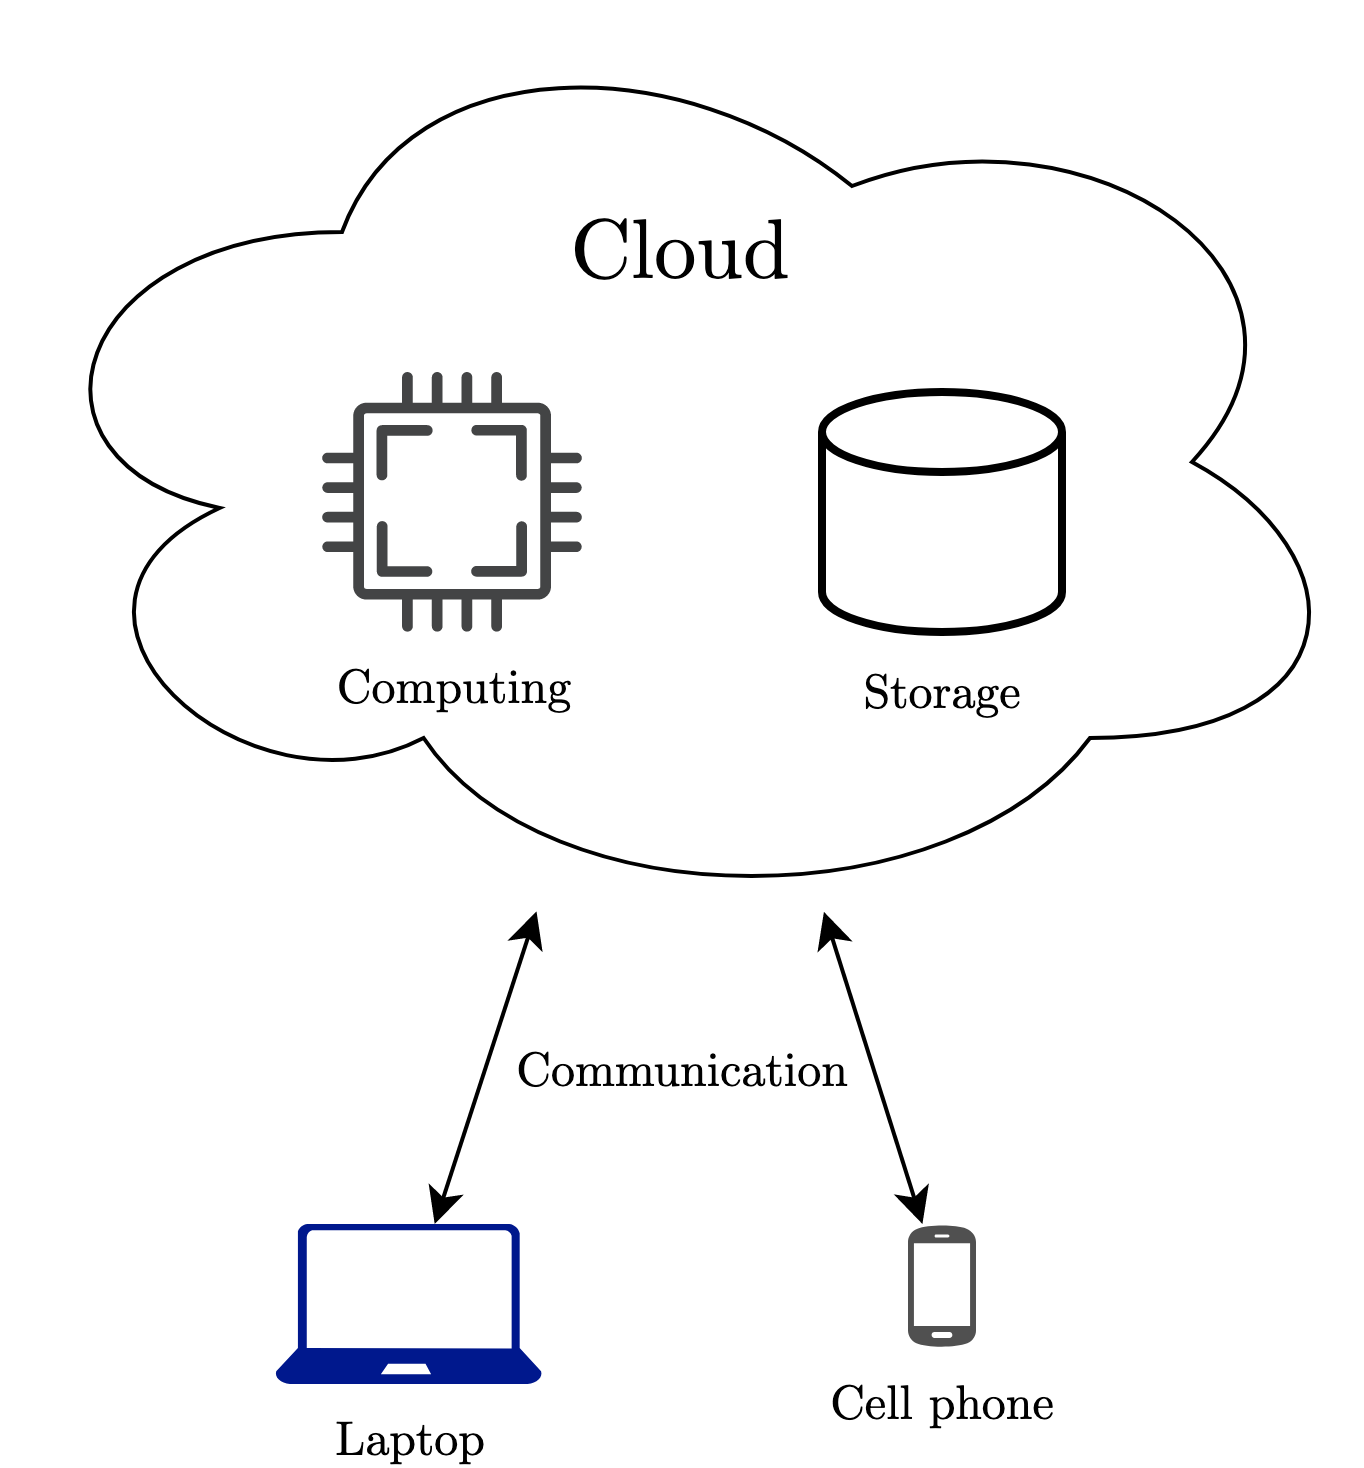
\includegraphics[scale=0.7]{chapters/background/figures/Simplified_cloud.png}
    \caption{A Simplified diagram of Cloud Computing}
    \label{fig:SimplifiedCloudDiagram}
\end{figure}

At a very high level, Cloud Computing is where you offload your work to the usually distant cloud. As shown on figure~\ref{fig:SimplifiedCloudDiagram}, a laptop or any other device can communicate with the cloud, and let the cloud provide storage and computation. The Cloud is a distributed system which is usually built as a Grid Computing system in a data centre. When working with the cloud, we typically have thin clients and thick clients. For traditional cloud computing the thin client is for example your laptop or cell phone, while the thick client is the server or servers in the distant data centre.

However, in today's society it has of course become much more advanced. You have an increasing number of cloud service providers that offer Infrastructure as a Service(IaaS), Platform as a Service(PaaS) and Software as a Service(SaaS), like Amazon Web Services(AWS), Digital Ocean, Alibaba Cloud, Microsoft Azure and Google Cloud Platform(GCP) just to name a few. The biggest of them all is AWS, which holds almost half of the market share\cite{noauthor_cloud_2019}. The Cloud market made 129 billion dollars in 2020 alone\cite{noauthor_cloud_nodate}.

Big firms will most likely benefit from building their own data centres. However most companies are not in the Fortune 500 with big wallets and millions of clients. Most firms, which have significantly less clients, can save a lot of money and time by outsourcing to cloud providers instead. It makes scaling easy and you can have infrastructure set up in just a few minutes, so you can focus on actually developing your service. You don't need to hire technicians to maintain the servers. If you have clients all over the world, you can choose to set up servers near them, instead of being limited to the office or headquarters. You can easily scale up by requesting stronger hardware, or you can easily scale out by replicating or starting more servers. In other words, it is just really convenient for most modern companies.

Even though the largest cloud providers have established themselves in many places, it still might not be close enough geographically to the client. In latency aware applications you need to minimize the physical distance between the client and the server. Therefore you can use local cloud providers, or firms like Akamai which specializes in having server as close, and as few as possible hops away from the end users.





% ----------------------------------------------





\section{Fog Computing}

Vaquero and Rodero-Merino\cite{vaquero_finding_2014}, defines fog computing like this: 
\say{Fog computing is a scenario where a huge number of heterogeneous (wireless and sometimes autonomous) ubiquitous and decentralised devices communicate and potentially cooperate among them and with the network to perform storage and processing tasks without the intervention of third parties. These tasks can be for supporting basic network functions or new services and applications that run in a sandboxed environment. Users leasing part of their devices to host these services get incentives for doing so.}

As in other fields, there is no de-facto definition and is debatable. Since Fog Computing is a relatively new concept, different definitions will be used depending on the field they are in.

Fog computing is an extension of the Cloud Computing paradigm. You have some nodes, like servers or desktops, that you offload the computation and storage to. The difference is that in Fog computing the fog nodes are located close in proximity to the user\cite{msftadmin_concept_2020}, as shown in figure~\ref{fig:FogDiagram}. The distant cloud has way more resources that the nodes in the fog layer, but since the fog nodes are closer, they are great at doing latency sensitive work. The Fog nodes is usually defined as being on the same LAN, but some argue that you can put them further away to, at least geographically speaking. 

An example is if an ISP has some Fog nodes at the base of cell towers. This will enable cell phones, or other SIM-card enabled devices, to offload storage and computation easily through the cell network. The introduction of 5G for the mainstream could benefit a lot from this. The latency for 5g will most likely be the same, but since the devices using it are so close to the 5G tower, it does not matter that much. The increased bandwidth of 5G is what will help a lot, as you can offload bigger workloads. We will discuss this in the Mobile Edge Computing chapter later. 

In Fog computing you would like as few jumps as possible to the node. A jump is when you move from one network node to another, for example from a cellphone to an Access Point. If the nodes are on the same LAN, the number of jumps are predictable and low in frequency, at least compared to the number of jumps to a distant data centre. 


For comparison, a Traceroute\cite{noauthor_traceroute68_nodate} from Oslo, Norway to a PlanetLab server in Rostock, Germany had at least 11 hops. With each hop adding latency because of processing, it’s easy to conclude that it is beneficial to keep hops at a minimum.

\begin{figure}[t]
    \centering
    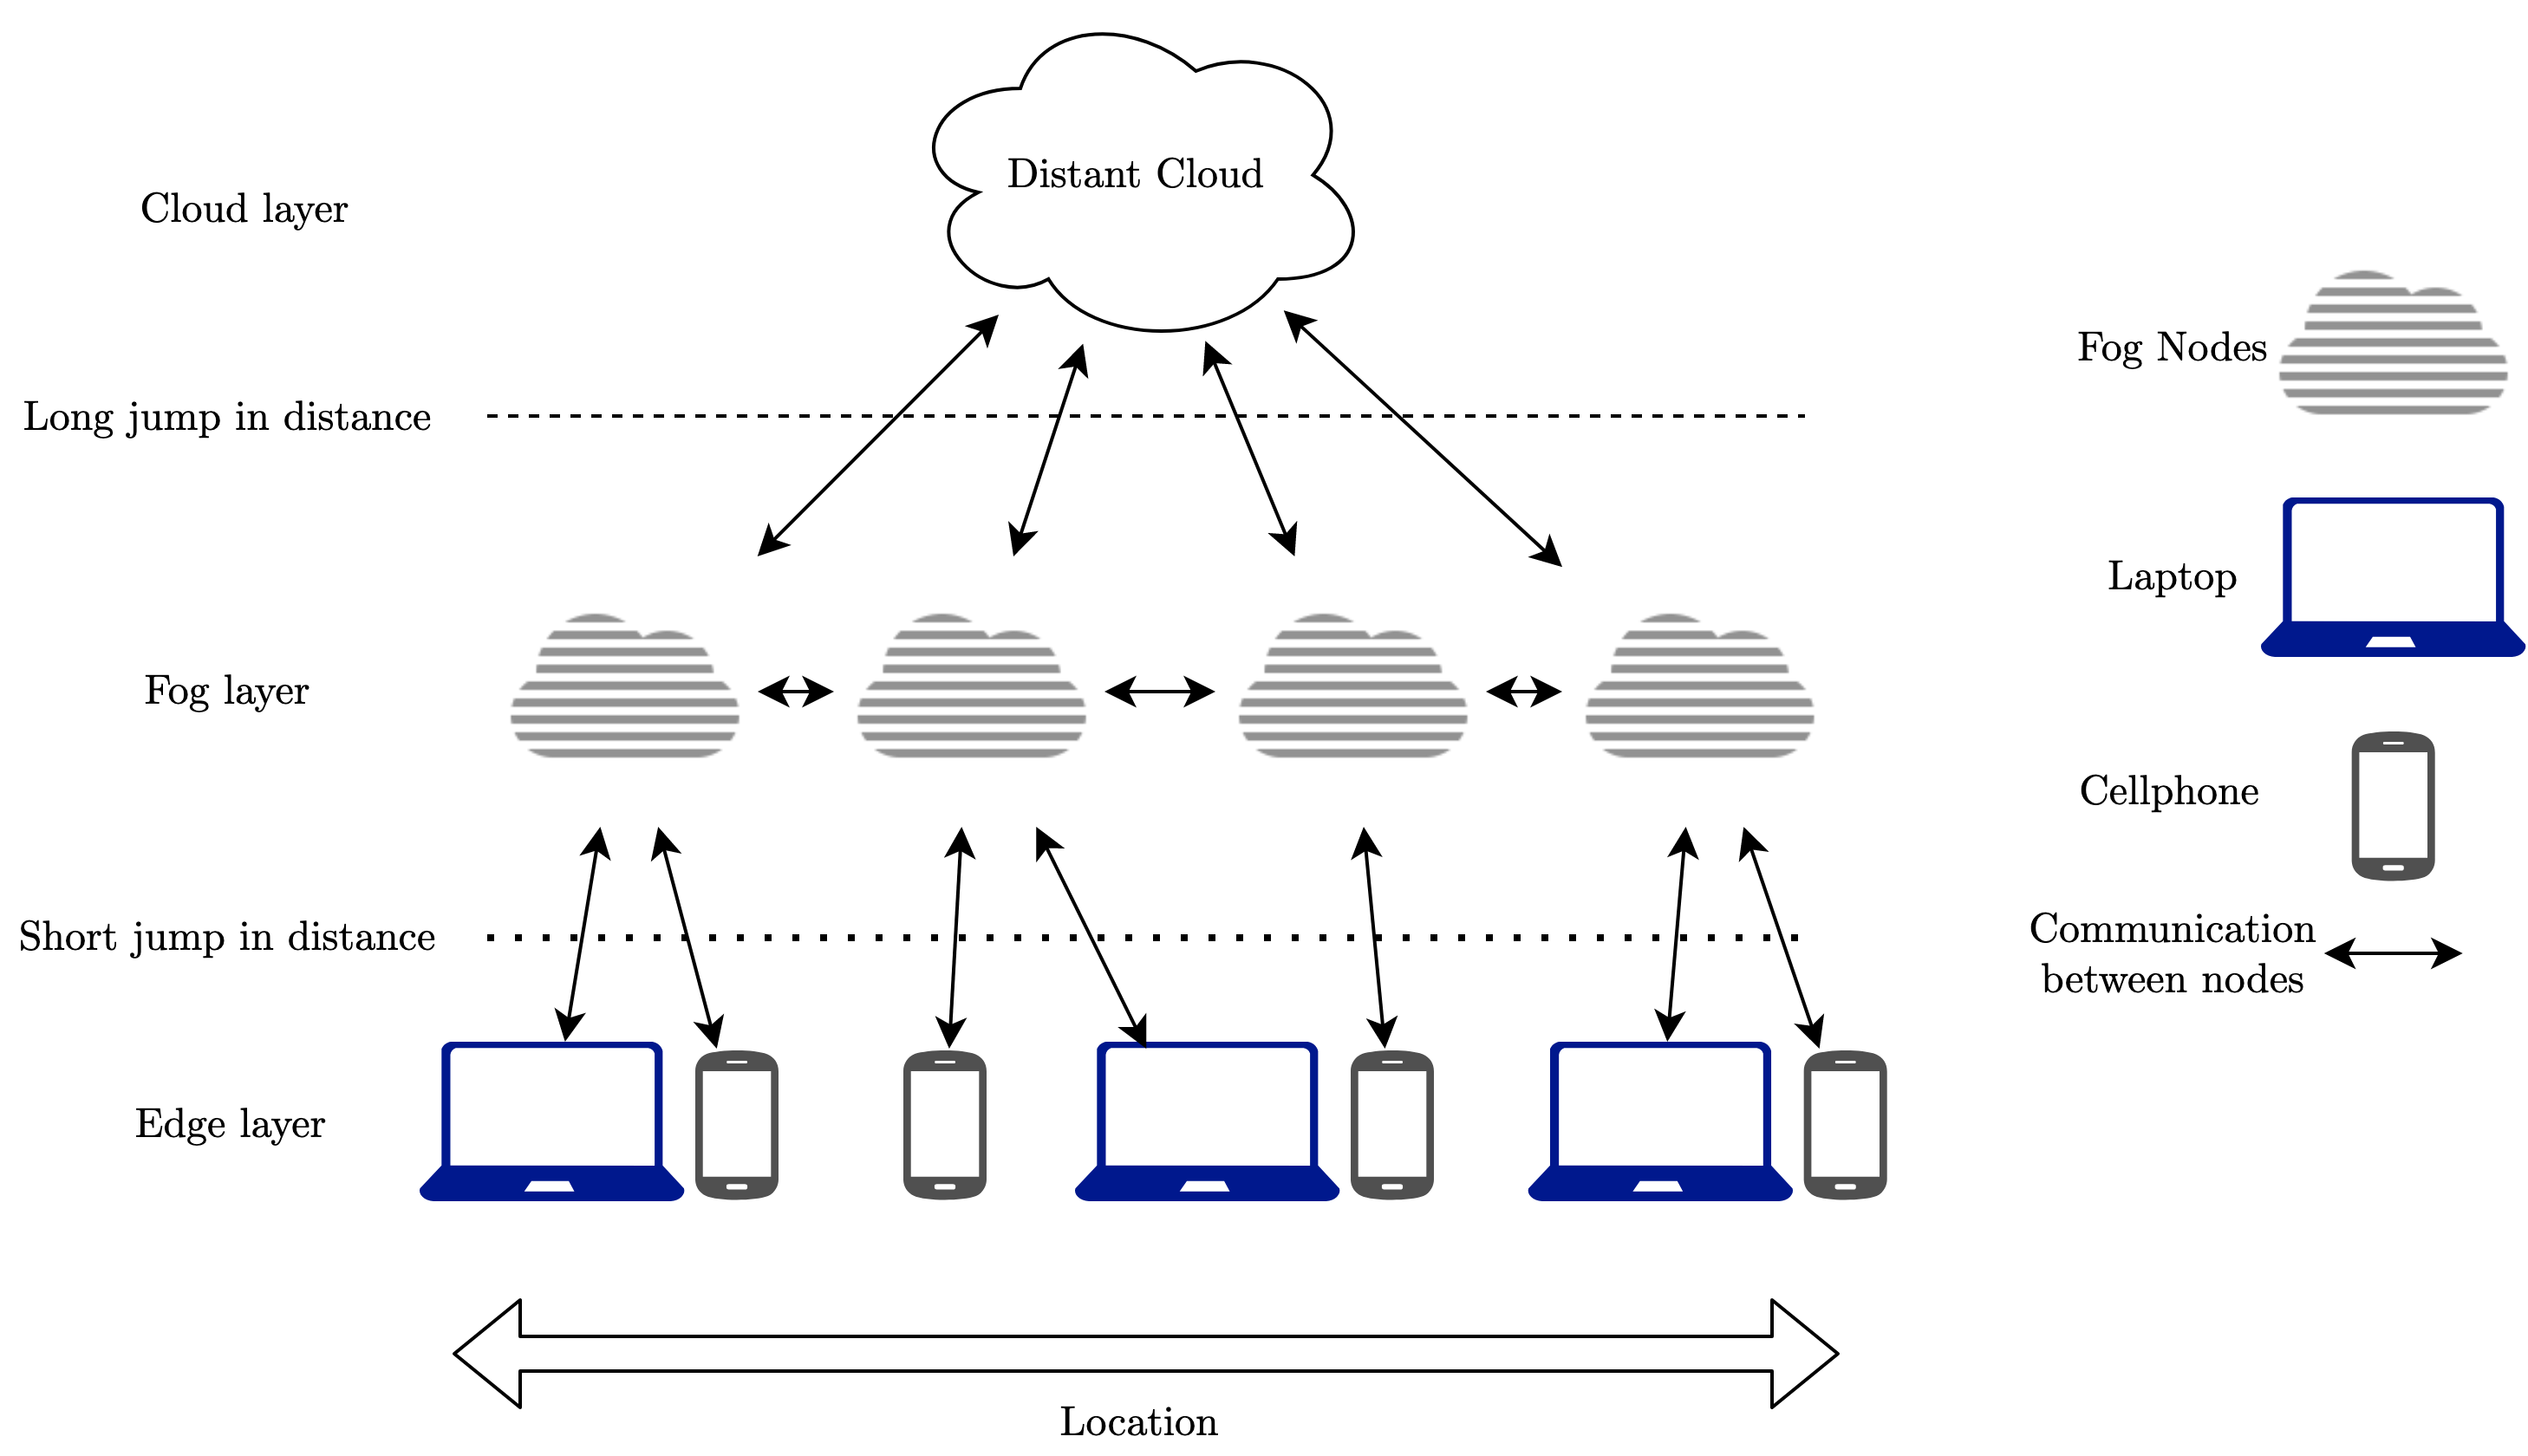
\includegraphics[scale=0.6]{chapters/background/figures/Fog.png}
    \caption{Diagram of Fog Computing}
    \label{fig:FogDiagram}
\end{figure}

\subsection{Cisco}
Cisco\cite{bonomi_fog_nodate} and Bonovi was the first to coin the term, and defines Fog Computing as \say{...a highly virtualized platform that provides compute, storage, and networking services between end devices and traditional Cloud Computing Data Centers, typically, but not exclusively located at the edge of network.}  The characteristics of Fog Computing is that it is located at the edge, has location awareness, low latency, easily geographically distributed, heterogeneity, support for mobility and some others. All these as a sum help with providing a service that is needed in some modern applications, for example Augmented Reality, and in general with IoT.

A Fog node is located at the edge in the sense that it is close to the end user or client. Because of this, the Fog node will have \textit{location awareness} and \textit{low latency}. Since they are not big servers, the Fog nodes are also easily \textit{geographically distributed}, in the sense that it should be easy to install and maintain. This also helps them be \textit{mobile}. Most likely the Fog nodes do not have the same hardware or software, which gives us the \textit{heterogeneity} characteristic. 

\subsection{A survey of Fog Computing} % TODO: REWRITE this
The goal of Fog Computing is to improve Quality of service(QoS) with computation and storage offloading. Yi, Li, and Li, in ‘A Survey of Fog Computing’\cite{yi_survey_2015} argues that QoS can be divided into four aspects: Connectivity, reliability, capacity and delay.

Connectivity in a fog network can be improved by network relaying, partitioning and clustering. They can be used to reduce cost, trim data and expand connectivity. Connectivity is of course important, because if you lose connection with the node, then you cannot offload work to it. 

Reliability is very difficult to provide in Fog computing. The methods used in traditional distributed systems like checkpointing and replication can be used. However since devices are more mobile, and nodes dynamic, this can be hard to implement. It also implies that Fog nodes are connected to each other, which is not given in all architectures. 

For capacity you need enough storage and good bandwidth. It does not matter how much storage you have, if it is slow to transfer it. To achieve good utilization of storage and bandwidth, it is important to analyse user patterns to know where data is most used. It’s difficult to know where to store data when it may need to be stored across several fog nodes. It is also hard to know when to send storage further to the distant cloud with bigger capacity at the cost of delay. 

Lastly, Fog focuses a lot on delay. It’s a good solution for “latency-sensitive” applications. There are several proposed solutions to minimize delay. We will discuss Cloudlets as a solution later.


% DETTE HØRER TIL I ARCHITECTURES
% \subsection{Fog architectures} %% move this to architectures?
% Naha et al.\cite{naha_fog_2018}, reviewed a couple of architectures that arguably falls under the Fog computing paradigm. We have focused on the ones that also fall under the Near-Far computing model, in that they have a Near node and a Far node. These architectures focus on offloading from an IoT device, to assist with computation, energy and storage. We will talk about IoT in a later chapter. 



% \subsubsection{Fog-Dew Computing (FD)}
% One drawback of Cloud computing is that you need to be always connected to the internet. 
% Fog-Dew Computing aims to provide IoT devices with cloud computing without being connected to the internet to reduce this issue. Depending on the application it might not need connection to the internet at all, while others can work temporarily offline but need to eventually connect to the internet. Fog-Dew Computing solves this by having an edge community server providing the needed cloud services. 




%----------------------------------





\section{Internet Of Things}
%TODO


\section{Edge Computing}
Edge Computing is about utilizing processing power at the edge of the internet, instead of using data centers. The edge of the internet are the devices that are closest to the users and clients. It's very relevant for IoT, because IoT end devices generate a lot of data close to the users but far from the data centres. This makes it very inefficient to send the data all the way to the distant cloud. Since IoT often requires real time processing of data, it is better to move the processing to the edge, closer to the devices, to minimize the latency\cite{shi_edge_2016}.
A router, switch or Cloudlet are examples of an edge device. They can be utilized by the IoT devices to offload their computation to save time and energy.


%TODO FJERN og snakk om dette i architectures?
\subsection{Content Delivery Networks (CDN)}
Content Delivery Networks are distributed systems that have servers geographically closer to the users. Akamai is a CDN company that specializes in bringing edge computing as close to the edge as possible. It has become widely popular, and a significant portion of the web moves through an Akamai device. They will have servers directly at the ISP’s so clients are just one “network hop” away from their servers. Akamai\cite{noauthor_exceptional_nodate} claims \say{85\% of the world’s Internet users are within a single “network hop” of an Akamai edge server.}. They also claim to handle 15-30\% of the world's web traffic. They help Netflix and similar companies to cache videos closer to the users so that they don't need to waste bandwidth across continents. They also help websites load faster and be more responsive, as the latency for getting the webpages are now minimal.


%% ----------------------------------------------------------------------



\section{The Near-Far computing model}
The Near-Far computing model is a cloud architecture that consists of a thin client that is connected to thick clients, which again is connected to even thicker clients. The Near-Far computing model covers a spectrum with nodes that are very close to you, like a cellphone in your pocket, and a node that is near you, like a desktop in the same room, as well as a distant data centre like AWS that is far away, most likely in another country. The spectrum covers distances from centimeters to several thousands of kilometers. Figure~\ref{fig:nearFarSimple} shows a pretty simple Near-Far setup, as well as the spectrum. In the Near-Far computing model you take the proximity of the Near server into consideration. You want the Near server to be as close as possible to the user. It can be a Cloudlet, which we discuss in section \ref{cloudlet}, for example. Optimally it is only one hop away, but considering cost and practicality, it can be more. The point is to minimize latency, but getting as close to the thin client as one hop is not feasible in every situation, especially on a tight budget.
%% HOW DOES NEAR FAR DIFFER FROM FOG?

\begin{figure}[t]
    \centering
    %\textbf{The Near-Far spectrum}\par\medskip
    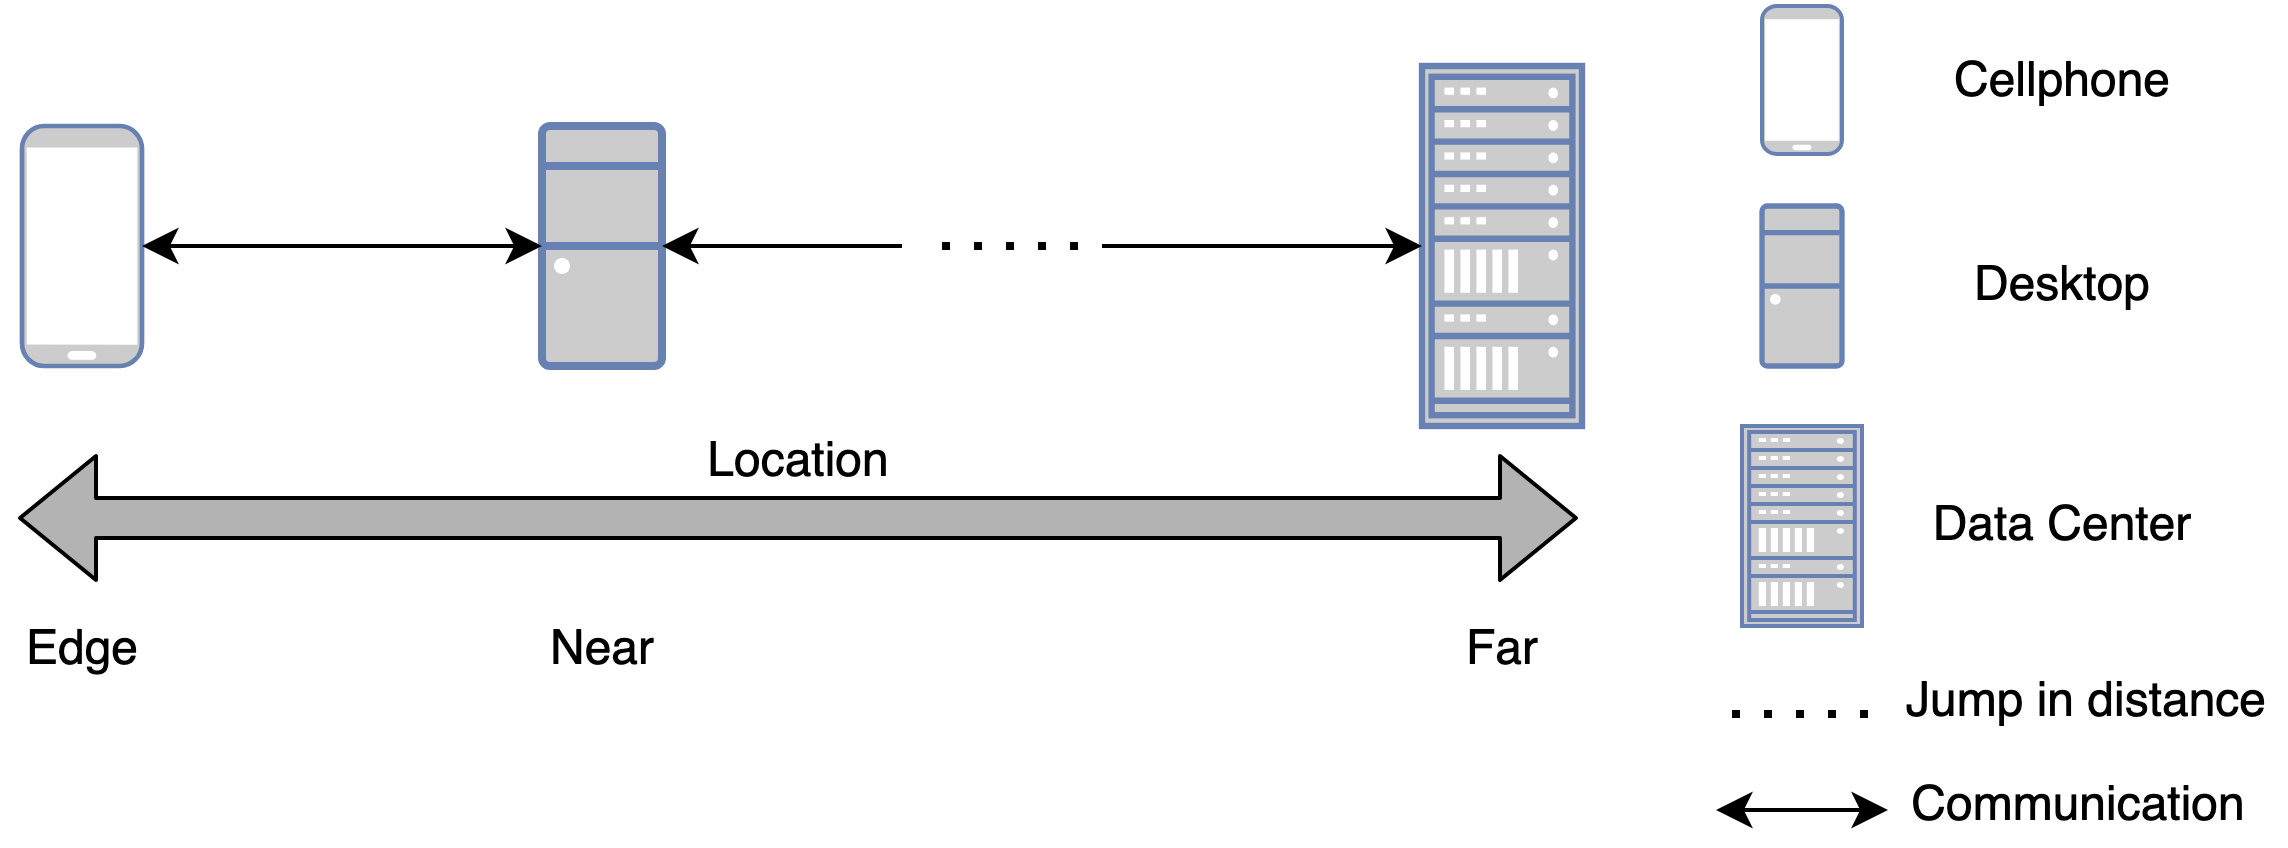
\includegraphics[scale=0.7]{chapters/background/figures/near-far-diagram.png}
    \caption{The Near-Far spectrum}
    \label{fig:nearFarSimple}
\end{figure}

%%---------------------------------------------------------------------

\section{The slow speed of light}
The speed of light in a vacuum is 299,792 458 kilometers a second. This is the upper limit for how fast anything can travel. This also limits how fast electrons can move in cobber and how fast light can travel in fiber-optic cables. Signals in fiber-optic travels at about 2/3 of the speed of light. The speed of electrons in a copper wire is slight faster than fiber. However, clock speed of computers today are in the billions of times per second. If you have a CPU running at 5GHz, in other words 5 billion clock cycles a second, we can see that the computer has time to do quite a lot while waiting for packets. When a packet has traveled just 1 foot, which takes 1 nanosecond, the CPU has already done 5 clock cycles. If the packet is traveling to another country, we can easily see that the CPU can do quite a bit of work while waiting for that packet. Since the speed of light is not going to change, the only way to improve latency is to reduce the physical distance between the nodes.



%% ----------------------------------------------------------------------------


\section{Why high latency and low bandwidth hurts}


Humans will easily detect delay and jitter when using applications\cite{satyanarayanan_case_2009}. Delay is almost impossible to fight when using hardware that is physically a long distance away. Jitter is impossible to prevent when using WAN. As a consequence, user experience of applications using WAN might suffer. Applications where crispness and high response time is important is called \textit{latency-aware applications}. Niraj Tolia et al.\cite{tolia_quantifying_2006} showed that we can divide user perceived responsiveness into several bins:
\begin{center}
\begin{tabular}{ | p{3cm} | p{5cm} | } 
    \hline
    Response Time& Perceived Responsiveness  \\ 
    \hline
    < 150ms & Crisp  \\ 
    150ms - 1s & Noticeable to annoying \\ 
    1s - 2s & Annoying \\ 
    2s - 5s & Unacceptable \\ 
    > 5s & Unusable \\ 
    \hline
\end{tabular}
\end{center}
The response time of applications is the sum of the time taken for packets to be sent between nodes, plus the processing time. Latency is not the only factor for how slow data transferring can be. Bandwidth is also a really important factor\cite{cerqueira_interactive_2007}. Some applications require very high bandwidth, that is not necessarily available everywhere. When bandwidth is too low, the transferring time will take longer, which then affects the response time. 
For latency-aware applications, keeping the application crisp is important. There of course exists applications that needs way lower response time than 150ms. Some applications require response time down to a few milliseconds. An example of this is when surgeons use a remote controlled robot to perform surgery. In this situation responsiveness need real-time to ensure safety. 







% ------------------------------------------------------------------------  

\section{Emerald}\label{Emerald}
Emerald is a programming language created in the period of 1984-1986 by Eric B. Jul, Norm Hutchinson, Hank Levy and Andrew Black. It has several features that is important in distributed programming, like object mobility and type conformity. These features helps easing the development process of distributed systems. Emerald is an example that you can have object orientation in distributed systems that have similar performance as C++ in many aspects. This section will give an introduction to Emerald, and are mainly based on the Emerald Language Report\cite{hutchinson_emerald_nodate}

\subsection{Types and Conformity}
When programming distributed systems, each node has to agree on how to handle data. Emerald does this with types and conformity. Each node does not need to transfer or have a copy of the whole object. It only needs to know what that object has available, which can be described with types. When calling a remote node, we just need to get a copy of the object type to be able to know what to call, and what to send. Having strong compile-time typing ensures that we will always get the expected data, which reduces errors and failures.

Everything is an object in Emerald. Even types are just first-class objects. 
Emerald is a compile-time strongly typed language. This means that the compiler will check that all objects conforms to the types at compile time, except for a few cases. An object conforms to a type if
\begin{enumerate}
    \item All operations defined in the type is available in the object
    \item For each operation, there are the same number of parameters, and each parameter conforms to the corresponding parameters.
\end{enumerate}
There are more checks, but these two are the most important ones.
Here is an example:
\begin{lstlisting}[language=emerald]
type TypeA
    Integer multiplyByTwo[n: Integer]
end TypeA

const ObjectA <- class ObjectA
    operation multiplyByTwo[n: Integer]
                        <- [res: Integer]
        res <- n * 2
    end multiplyByTwo
end ObjectA
\end{lstlisting}
Here, the ObjectA conforms to TypeA because we have the \textit{multiplyByTwo} operation, the type of the parameter and the type of the return is the same as described in the type.

To enable generic types and polymorphism, Emerald lets you also check types during runtime with an operator: \verb|*>|. You can essentially read \verb|a *> b| as "\textit{a} conforms to \textit{b}". You also have \verb|view a as b| to help change the type of an object during runtime.




\subsubsection{Classes}
Emerald does not really have classes as everything is an object. We still have the concept of classes, and Emerald has the keyword \verb|class| to help us easily create it. Emerald will automatically create a type, a \textit{getSignature} operation, which returns the type, and finally a \textit{create} operation. These two objects are therefore semantically equivalent:
\begin{lstlisting}[language=emerald]
const A <- class A[x: Integer]
    export operation multiplyByTwo[n: Integer]
                        -> [res: Integer]
        res <- n * 2
    end multiplyByTwo
end A

const B <- object B
    const BType <- immutable typeobject BType
        operation multiplyByTwo[n: Integer]
                            -> [res: Integer]
    end BType
    export function getSignature -> [r: Signature]
        r <- BType
    end getSignature
    export operation create[x: Integer] -> [e: B]
        e <- immutable object aB
            export operation multiplyByTwo[n: Integer]
                        -> [res: Integer]
                res <- n * 2
            end multiplyByTwo
        end aB
    end create
end B
\end{lstlisting}
As you can see, using the \verb|class| keyword dramatically increases readability, gives us the consept of classes, and eases the development.

\subsection{Fields}\label{emerald:fields}
Emerald provides the keyword \verb|field| to automatically provide getters and setters.
\begin{lstlisting}[language=emerald]
const A <- class A
    field someVar : String <- ""
end A

const B <- class B
    var someVar: String <- ""
    
    export op getSomeVar -> [res: String]
        res <- someVar
    end getSomeVar
    
    export op setSomeVar[input: someVar]
        someVar <- input
    end setSomeVar
end B
\end{lstlisting}
In the above example, both class A and class B is equivalent. They will both have the operations \verb|getSomeVar| and \verb|setSomeVar| available.


\subsubsection{Immutability}
To ensure that objects does not change over time, we need immutability. This is important in distributed systems, as changing an object that was not meant to change can break how it is supposed to interpret data, as we can have nodes with different versions of the object. Since Emerald only copies over the type to other nodes, it is important that these types are not able to change(mutable). Therefore, all types should be mutable. Classes should be immutable if possible, to prevent confusion between nodes. The less mutable objects there are, the less errors and failure there can be.

\subsection{Object mobility}
One of the key features of Emerald is Object Mobility. It has the tools needed to easily move objects around in a distributed system. To move an object to a different node is as easy is this:
\begin{lstlisting}[language=emerald]
% x is created and resides on A
move x to B
% x now might reside on B
\end{lstlisting}
To visit all available nodes with your program is as easy as this\cite{noauthor_emerald_nodate}:
\begin{lstlisting}[language=emerald]
const Kilroy <- object Kilroy
  process
    const origin <-  locate self
    const up <- origin.getActiveNodes
    for e in up
      	const there <- e.getTheNode
      	move self to there
    end for
    move self to origin
  end process
end Kilroy
\end{lstlisting}
This short and simple compilable and runnable Emerald program will start a process, find all active nodes and then loop over and visit them, before going back to the original node.

The move keyword is more of a hint to the Emerald VM that the object should be moved over. In Emerald you can use \verb|fix| to tell the VM that it has to move the object, instead of it just being a hint. It has the same syntax as move:
\begin{lstlisting}[language=emerald]
% x is created and resides on A
fix x at B
% x now resides on B, and will not move until unfixed.
\end{lstlisting}
To move the object again, we now have to unfix it, which is done by using \verb|unfix|:
\begin{lstlisting}[language=emerald]
unfix x
\end{lstlisting}
The object can now be moved or fixed on a different location. To make this procedure easier we have the \verb|refix| keyword. It will unfix and then fix an object to a new location. In other words these are equivalent:
\begin{lstlisting}[language=emerald]
unfix x
fix x at C
\end{lstlisting}
and
\begin{lstlisting}[language=emerald]
refix x at C
\end{lstlisting}
Therefore we use refix almost everywhere when we are moving objects. 



\subsubsection{Attached}
When moving objects in Emerald, you are essentially just moving the pointer. This means that if you have an object with some inner variables, they will stay on the original node when the parent is moved. If it makes sense to move the related data with the object, which it usually does, we can use the \verb|attached| keyword.
As shown in figure~\ref{fig:emerald_attached_figure}, when using the Attached keyword, both the object and the attached objects will move over, when that parent object (x) is moved. If we do not move the related objects over, then there will be a tremendous performance impact because local invocations are many times faster than remote invocations. Here is an example of how you can use attached:
\begin{lstlisting}[language=emerald]
const x <- class x
    attached const y <- someObject.create
    attached const z <- someObject.create
end x
\end{lstlisting}
In the above code example, you will get an object similar to the one shown in Node A in figure~\ref{fig:emerald_attached_figure} before the move.

\begin{figure}[t]
    \centering
    \textbf{Not attached vs Attached}\par\medskip
    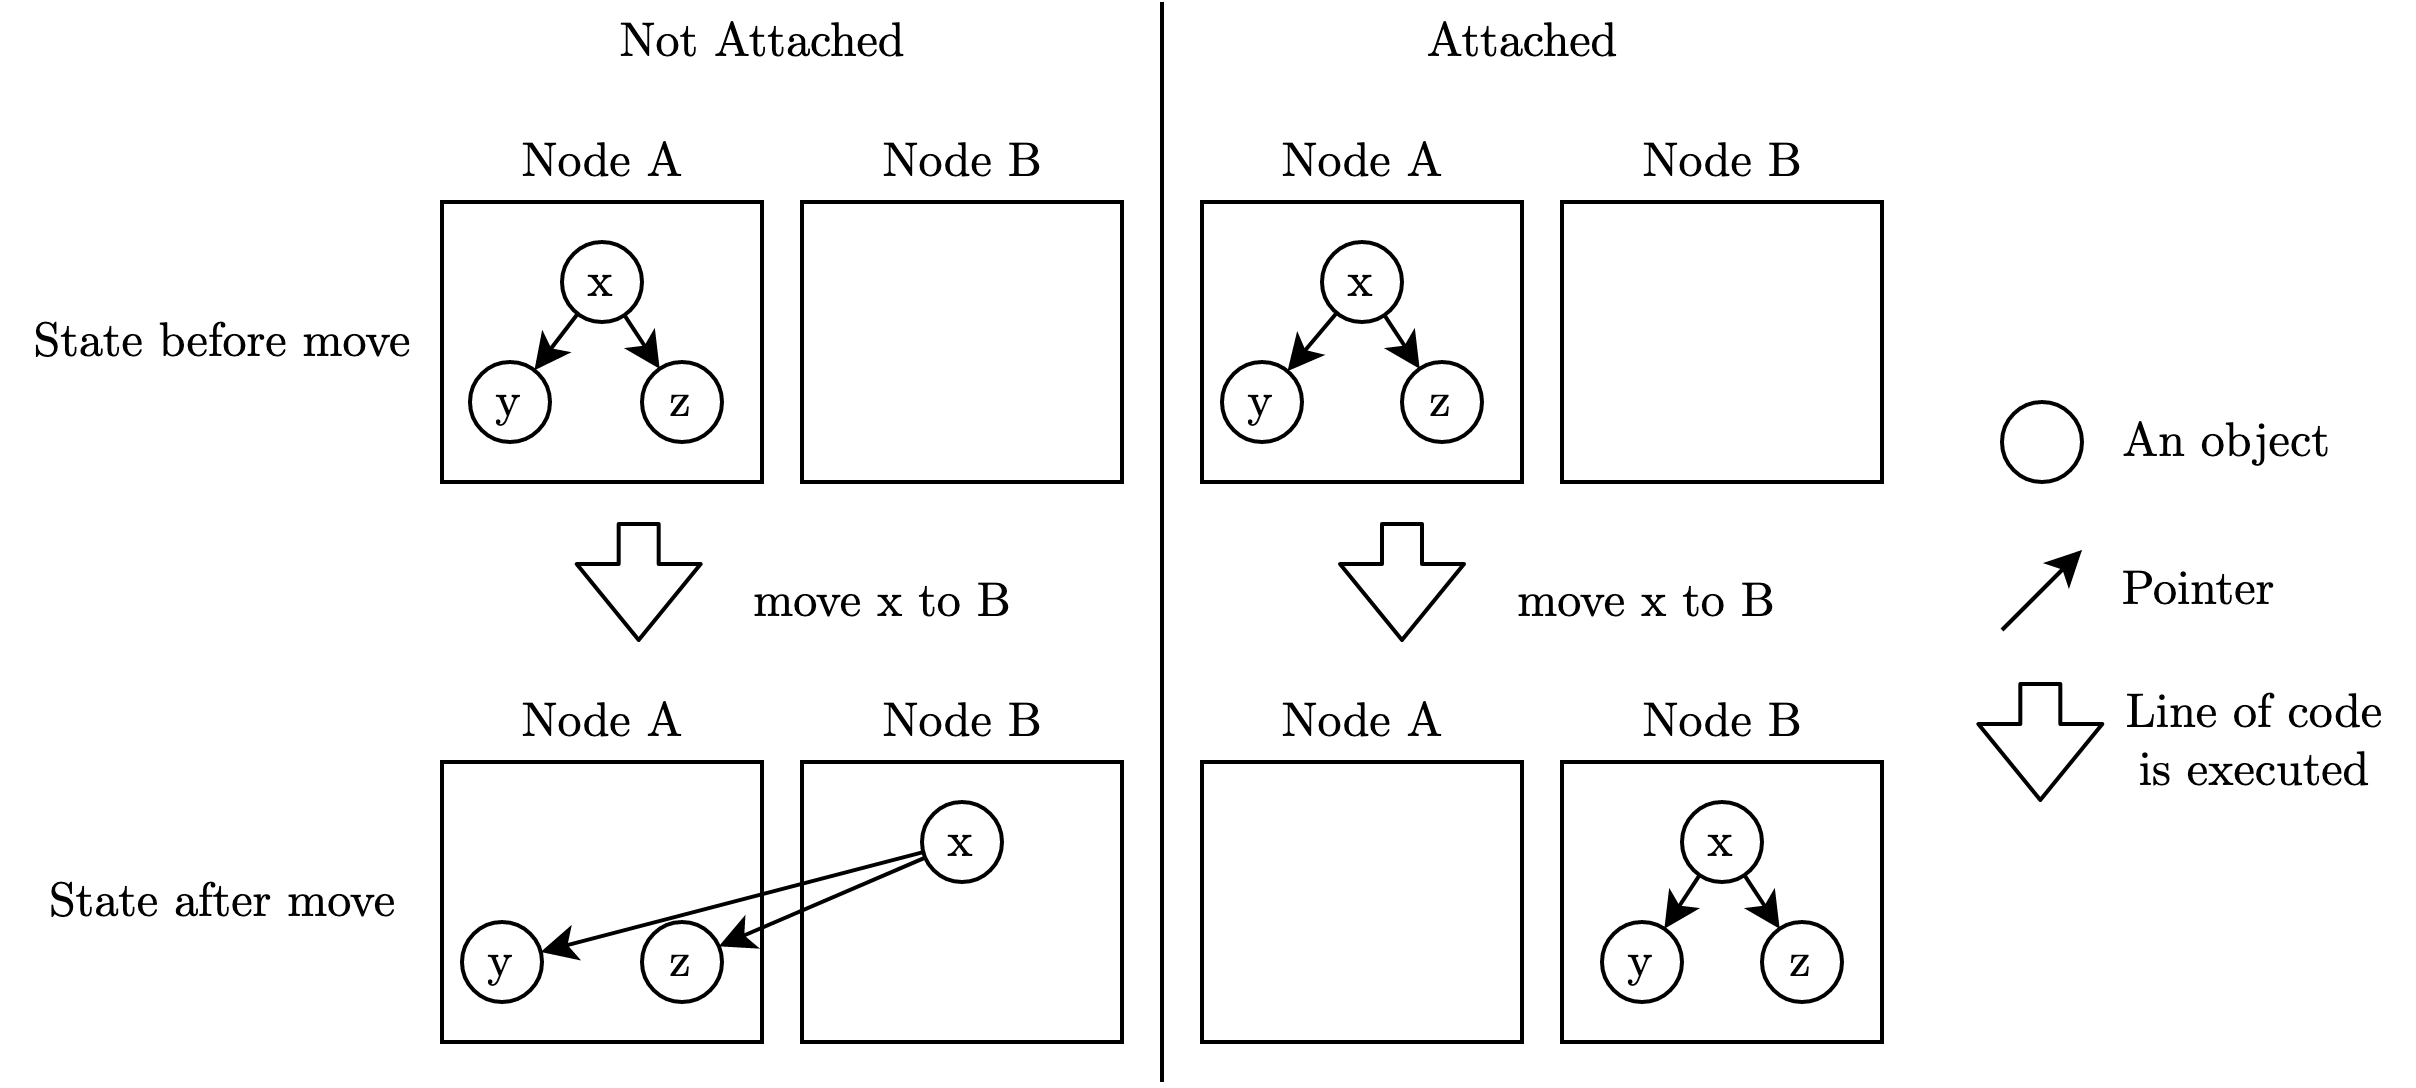
\includegraphics[scale=0.8]{chapters/background/figures/emerald_attached.png}
    \caption{Showing a move executed without and with attached objects}
    \label{fig:emerald_attached_figure}
\end{figure}

\subsubsection{Call-by-visit and call-by-move}
Call-by-visit and call-by-move are very similar concepts as attached. In Emerald you can use them to specify when you want to move the objects you send as parameters when invoking a function on a remote node. When using call-by-visit you move the parameters over, then move then back when finished with the function. When using call-by-move, you do the same, except the object stay on the remote node.

\subsubsection{How the Emerald VM finds the location of objects}\label{cascading_search}
Emerald has a system for keeping track of and finding objects. To get the location of an object you can use the \verb|locate| keyword. For example:
\begin{lstlisting}[language=emerald]
const x <- 3
move x to B
var locationOfX : Node <- locate x
% The variable "locationOfX" now holds 
%  the Node object that resides on B.
\end{lstlisting}
Emerald uses something called \textit{Cascading Search} to locate an object. To prevent having to broadcast each time an object moves, a node only keeps track of the last position it knows the object resides or resided on. If the last known position of X is on A, then we just ask the A if he can send it. If A has later moved X to node C, then it will just send the query to C. This is called a Forwarding Reference. It keeps track of last known location (from its own perspective) and also a counter. Each time an object moves, that counter is incremented on the receiving node. If node A moves object X to B, then the counter is 0 at A and 1 at B. That means that the higher the counter, the more recent the pointer is. The counter is essentially replacing a global clock, since having synchronized time is almost impossible in a distributed system. The algorithm also have ways of dealing with failing nodes and lost pointers, but we wont go any deeper into that. 


\subsection{Remote Procedure Call}
Emerald uses Remote Procedure Calls, which means that it will handle all remote invocations for you. Therefore, when programming, you can just invoke the object as if it were local. This ensures that programming with distributed objects is really easy, as you do not need to think about programming each remote invocation. Here is a comparison:
\begin{lstlisting}[language=emerald, numbers=left]
const A <- class A
    export function multiplyByTwo[i: Integer] 
                                -> [res: Integer]
        res <- i * 2
    end mulitplyByTwo
end A

const B <- object B
    initially
        const x <- A.create
        % x is now a local pointer to A
        const result1 <- x.multiplyByTwo[2]
        
        refix x at someOtherNode
        % x is now a remote pointer to A
        const result2 <- x.multiplyByTwo[2] 
    end initially
end B
\end{lstlisting}
On line 12 and 16, we do the same invocation, but the location of the invoked function is different.

If we try to invoke a function on a node that is not available, Emerald will raise 




\subsection{Failure and Unavailable}
When programming distributed systems we need to account for nodes going up or down. To help with this, Emerald has introduced \textbf{unavailable handlers}. Unavailable handlers can be put at the bottom of process blocks, functions and compound blocks. Within an unavailable handler, one can try to recover by trying again or by trying other nodes, for example.

\textbf{Failure Handlers} are invoked when a failure is raised by the program. An example of this is when invoking a nil object. The failure handler can be used to try to recover the program.

Below is an example of both failure and unavailable handlers:
\begin{lstlisting}[language=emerald, numbers=left]
const A <- class A
    export function divideTwoBy[i: Integer] 
                                -> [res: Integer]
        begin %compound statement
            res <- 2 / i
            failure
                % This will be executed if i is 0
            end failure
        end
    end mulitplyByTwo
end A

const B <- object B
    initially
        const x <- A.create
        % x is now a local pointer to A
        const result1 <- x.divideTwoBy[0]
        
        refix x at someOtherNode
        % x is now a remote pointer to A
        const result2 <- x.divideTwoBy[0]
        
        unavailable
            % this will be executed if someOtherNode
            %  is unavailable
        end unavailable
    end initially
end B
\end{lstlisting}






\subsection{Checkpoints and Recovery}
To help keeping nodes up, Emerald provides checkpoints and recovery blocks. At any point you can use the reserved \verb|checkpoint| keyword to create a checkpoint of an object. The checkpoint is just a saved state on the machine, so that the state is available on the disk instead of just RAM. If a node has restarted, then it will load the last checkpoint. When the program is recovering, the \verb|recovery| block is ran instead of the initially block. This is essential for creating more reliable distributed systems.



\subsection{Concurrency}
Emerald has support for processes, and they are really easy to set up. You use the process block like this:
\begin{lstlisting}[language=emerald]
const A <- class A
    process
        % do work here
    end process
end A
\end{lstlisting}

Emerald has also implemented monitors based on Hoare's monitors\cite{hoare_monitors_1974}. You can use the keywords \verb|monitor|, \verb|wait|, \verb|signal| and the \verb|Condition| type to easily have control over concurrency. Here is an example:
\begin{lstlisting}[language=emerald, numbers=left]
const A <- monitor class A
    const cond: Condition <- Condition.create
    export function multiplyByTwo[i: Integer] 
                                -> [res: Integer]
        wait cond % wait for your turn
        res <- i * 2
        signal cond % signal to _one_ other process
    end mulitplyByTwo
end A
\end{lstlisting}
In this example, line 6 will not be executed at the same time as other processes.







\subsection{Compiling and running}
You can compile Emerald with the Emerald Compiler\cite{noauthor_emeraldold-emerald_2019}, which, when installed, can be run in a terminal with \verb|ec|. When you have written you program you compile the files with \verb|ec| like this:
\begin{lstlisting}[language=Bash]
ec file1.m file2.m 
\end{lstlisting}
To then run the program, you use the \verb|emx| which will run the compiled program on the Emerald VM:
\begin{lstlisting}[language=Bash]
emx file1.x file2.x
\end{lstlisting}

To start a remote node, run this on the remote node:
\begin{lstlisting}[language=Bash]
emx -U -R
\end{lstlisting}
Then all the other additional nodes is started like this:
\begin{lstlisting}[language=Bash]
emx -U -R172.17.0.2
\end{lstlisting}
Here \textbf{172.17.0.2} is the IP address of the first node.
Finally, to run the program run this:
\begin{lstlisting}[language=Bash]
emx -U -R172.17.0.2 file1.x file2.x
\end{lstlisting}
All the other nodes are now accessible, and can have objects moved to them.



%% ---------------------------------------------------------

\section{Docker}\label{background:docker}
Docker is a tool for running programs on the same architecture everywhere, without spinning up a whole virtual machine. It is built around the concept of \textit{containers}. Containers are small packages of software, that run on the Docker Engine. The Docker Engine is the the middleware between the containers and the operating system. This lets us run something locally and be able to expect the same behavior on other machines. Therefore, no matter where you run the application, it will always be the same environment from the perspective of the program. 

Because a Docker does not spin up a whole virtual machine, but rather share some resources with between the containers \cite{dockercom_what_nodate}, it is more efficient. The container is essentially a sandbox, that runs on top of the OS. Each of the applications are therefore isolated, even though they have some shared resources.

To run Emerald we use a stripped debian image with i386 architecture, made by Oleks Shturmov\cite{oleks_oleksdocker-in5570v21_2021}.
In the referenced github repository, Oleks provides a makefile to easily set up Emerald.



%%------------------------------------------------------
\section{PlanetLab}
PlanetLab is virtual organization consisting of many nodes spread out over the world. If an institution, like an university, wants to use PlanetLab, then they have to provide a PlanetLab server themselves. In other word, the institution get sent a server, which they have to install and maintain to keep using PlanetLab. This ensures that you get a wide network that spans all over the world. At it's peak, it had 1353 nodes spread across the earth\cite{noauthor_planetlab_nodate}. It is used as a wide-area network to do research on distributed systems. To get access you request for a DIKU, which is a collection of servers that you can log into. The login username for the servers, is then the name of the DIKU.

Each of the nodes run some from an operating system. We can connect to them with Secure Shell(SSH). Each node we use in this thesis will have Docker available. To run Emerald on a PlanetLab server, transfer the Emerald source code or executable and the makefile for running Emerald, over to the server with scp. For example, transfer the folder you are currently in to the home folder on the remote server:
\begin{lstlisting}[language=Bash]
scp -r . "planetlab-1.ida.liu.se":"~/"
\end{lstlisting}
Then ssh into the server: 
\begin{lstlisting}[language=Bash]
ssh -i ~/.ssh/planetlab \
    -l diku_name \
    "planetlab-1.ida.liu.se"
\end{lstlisting}
Here we provide a PlanetLab ssh key and the login name, which is the name of the DIKU, and a server URL.

When logged in on the server, we run the makefile with \verb|make| to start the shell within the Docker container. Then you can either run the executable, or compile the code as described in the Emerald section \ref{Emerald}.



\section{Summary}
In this chapter we have made a theoretical foundation to help understanding this thesis. We have described what a distributed system is, what it consists of, and some key features about it. We have given a short introduction to Edge, Fog and Cloud computing. We have also made a short description of Near-Far computing, explained what speed of light have to do with latency, and showed how the Emerald eco-system works. Finally we have given a description of the environment the experiments will be conducted on, with Docker and PlanetLab.

%% TODO:

%% LAG FIGURES TIL DISTRIBUTED SYSTEMS

% Snakk om Why latency hurts? Snakk om hvorfor vi offloader?

% iot

%NFV og SDN? 


\chapter{Design of experiments}\label{chapter:design_of_experiments}
% how to do the experiments etc
% methodology
 %% “Plan for empirical studies”,“Design of experiments”
%% this chapter describes how and why we evaluate this way

\section{Scope}
Our goal of these experiments is to show how the Near-Far Computing Model relates to already existing architectures. We will develop several of the architectures in Emerald, and then conduct experiments on them. We will analyze and measure how the architectures tackle latency problems. 





\section{Simulation}
We will simulate the different architectures using Emerald and PlanetLab. The Emerald programming language will be used to make a high level version of these architectures. This comes with a bonus, namely that the Emerald VM is working as middleware for these experiments. This makes it easier to show experiments, as the code is easily understood and the architectures will be reduced to something that is easily tested.








\section{Experiments}
To show the viability of the architectures we will benchmark and analyze some factors:
\begin{itemize}
    \item Latency
    \item Reliability?
    \item Distribution Transparency
    \item Computational usage
    \item Storage
    \item TODO: need more here
\end{itemize}
% Hvordan kan man måle reliability?



\subsection{Latency}
Latency will be mapped by recording the round trip time in milliseconds. Doing this is really easy, as we can just record the time before sending work, and then recording the time when we get the result. If time at send is $T_0$ and time at receive is $T_1$ then latency gets this easy formula:
\[Latency=T_1-T_0\]
There is a slight overhead for actually taking this time, but it is marginal compared to the milliseconds of latency. Here is a small program which just takes time $T_0$ and $T_1$ and just prints the difference:
\begin{lstlisting}[language=emerald, numbers=left]
const main <- object main
  initially
    const home <- locate self
    const t0 <- home$timeOfDay
    const t1 <- home$timeOfDay
    home$stdout.PutString[
        "Total time " || 
        (t1-t0).asString ||
        "\n"]
  end initially
end main
\end{lstlisting}
Output:
\begin{lstlisting}[language=Bash]
$ emx latency_overhead_test.x
Total time 0:000002
\end{lstlisting}
As we can see, there is just 2 microseconds of overhead.
When there is several nodes, we will map these latency's as needed to be able to compare each architecture.

\subsection{Reliability}
TODO
%Simulere støy? F.eks, de som bruker base-stations så kan jeg si at så n så mange pakker må sendes på nytt?

\subsection{Transparency}
Since Distribution Transparency is more about key features, it makes little sense to measure it quantitatively. We will therefore compare transparency characteristics from each architecture instead. We will take the different transparencies we talked about in section \ref{distributed_systems} in the background, and lay out how the different characteristics relate to these.


\subsection{Computational usage}
We will compare how much computation each group of nodes in the architectures is using. Specifically, we will see how much the end client, the near nodes and the far nodes are being used. This is to show how the load is spread across the nodes in the different architectures. For example, the end user are using 20\%, the near node(s) are using 70\% and the far node(s) are using 10\%.
TODO: how do we benchmark this?

\section{Storage}
We will compare how viable the architecture are for offloading storage. We will measure how fast it can offload and download data.



\bigskip
TODO:
\begin{itemize}
    \item several architectures  
    \item Create a program in emerald  
    \item benchmark  
    \item How it relates to the near-far computing model  
    \item quantitaive data  
    \item Compare to the background of distributed systems, like how transparent it is  
    \item PlanetLab  
    \item Emerald  
\end{itemize}




\section{Summary}
TODO: summaryyy



%Notes:
% Hvis vi mangler info å skrive om kan vi skrive om storage?



\chapter{Architectures}\label{chapter:architectures} %% implementation and design
%% one of the architecutres should be based on replication?

%% cloudlet?
%% MAUI?




\section{Multi-Access Edge Computing}
Multi-Access Edge Computing(MEC), also known as Mobile Edge Computing, was originally an architecture that proposes to utilize the cellular network for having a close-by MEC server\cite{porambage_survey_2018}. An MEC server is a server that has software and hardware designed to handle work and storage offloading. However, this has later extended to include WiFi as well, as more and more IoT devices are connected to either cellular of WiFi. If needed, a distant data centre or CDN can aid the MEC server with even more storage and computation.
\begin{figure}[t]
    \centering
    %\textbf{Mobile Edge Computing}\par\medskip
    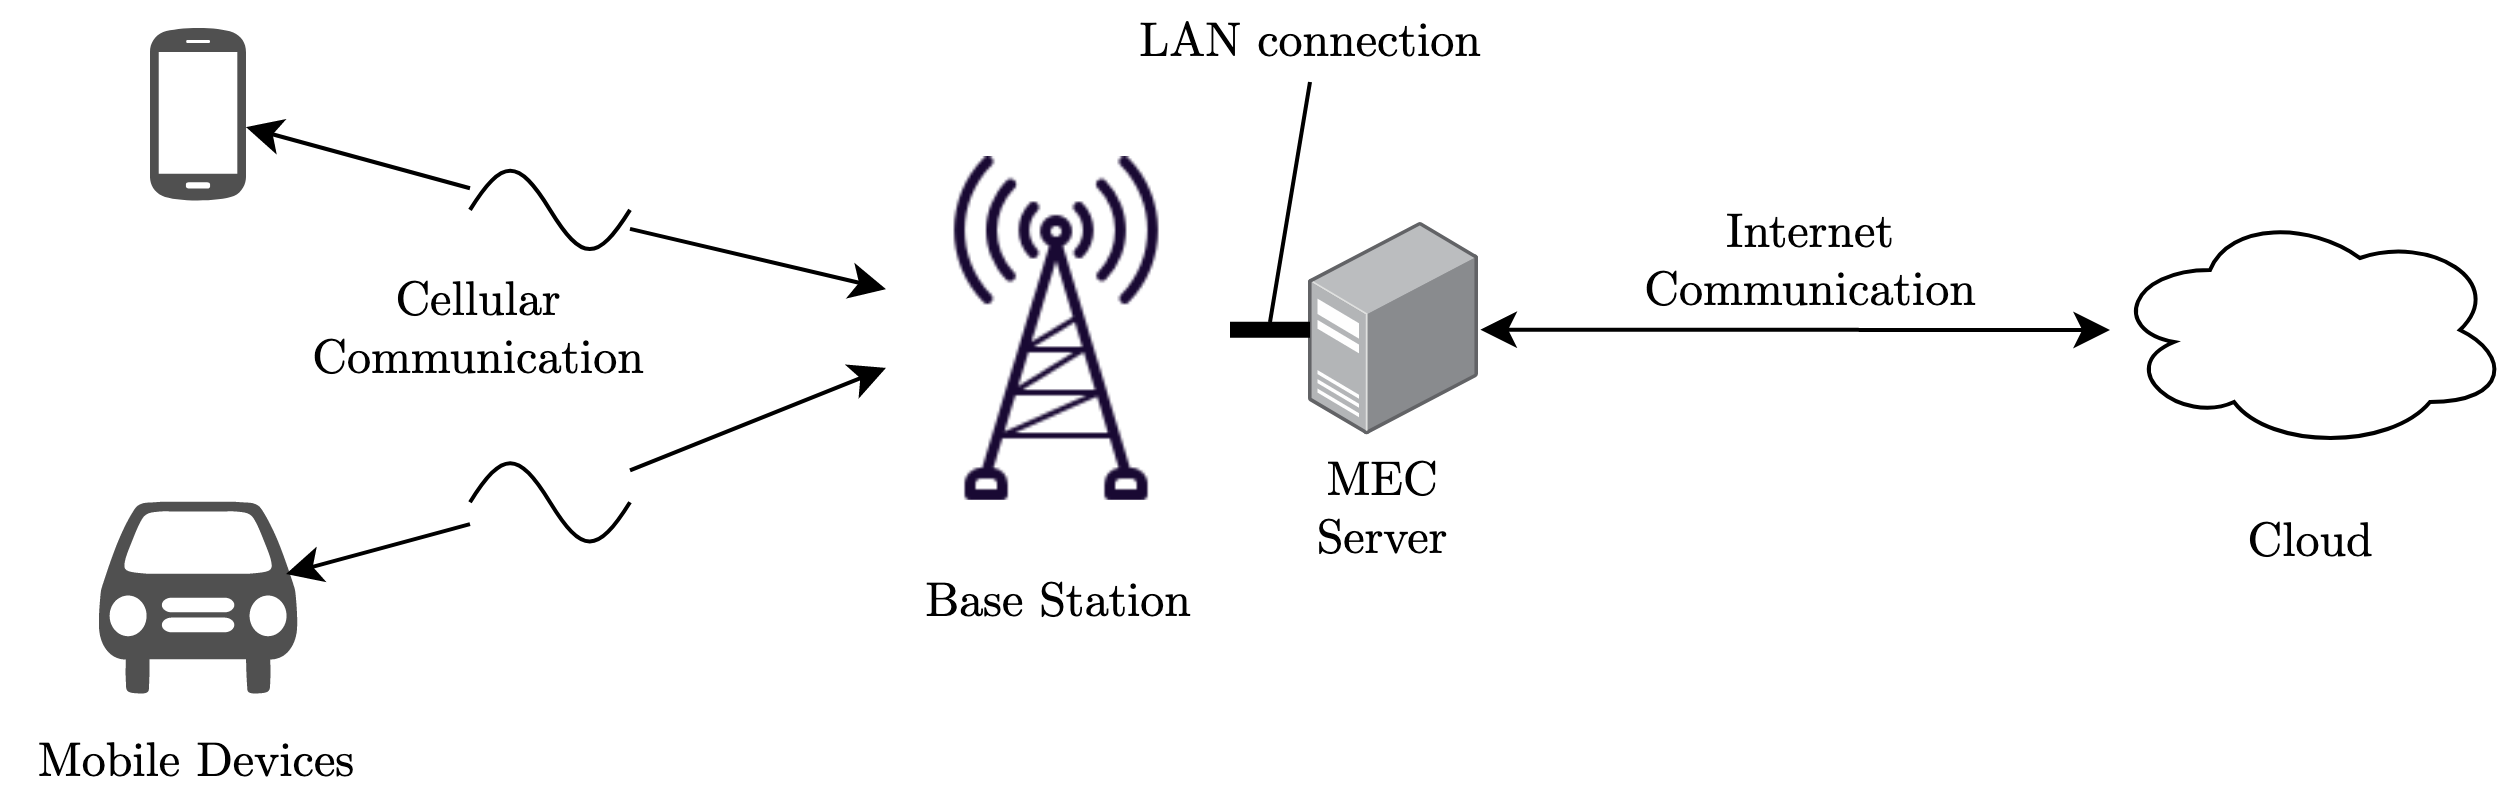
\includegraphics[scale=0.75]{chapters/architectures/figures/MEC.png}
    \caption{Diagram of MEC}
    \label{fig:MEC}
\end{figure}

Figure \ref{fig:MEC} shows how MEC works on a high level. MEC will utilize the ubiquitous cellular network to offload its work. At the base station there will be a MEC server that can provide storage and computational power to the mobile devices. However, the base station servers is not as powerful as the distant cloud servers. Since the base station is just one hop away, we don't have to deal with the dynamic wide-area network. Additionally, the cellular network provides a very small delay, as base stations are relatively close by to almost everywhere where there are developed civilization. If the servers at the base station are overloaded they can send the work further to the data centres of the distant cloud or a CDN. The mobile devices can be any type of device that need storage offloading. The only requirement for this architecture is that it has a cellular or WiFi connection.

The MEC server architecture is divided into several layers that together forms three systems\cite{patel_mec_nodate}. At the bottom is the hardware layer. Over that is the virtualization layer. These two layers is part of the MEC Hosting Infrastructure Management System. Over that is the MEC Application Platform Management System which consists of a MEC virtualization manager layer and and MEC Application Platform Services layer. The virtualization manager can provide IaaS. The MEC Application Platform Services layer is an interface for the virtual machines that the applications is running on. The VMs and the apps form the Application Management Systems. Figure \ref{fig:MEC_Server} is a simplified version of the server architecture presented in \cite{patel_mec_nodate}. It shows that we can have several applications running simultaneously on the MEC Server. All the Applications run in a VM that is controlled by the MEC Application Platform Services.
\begin{figure}[t]
    \centering
    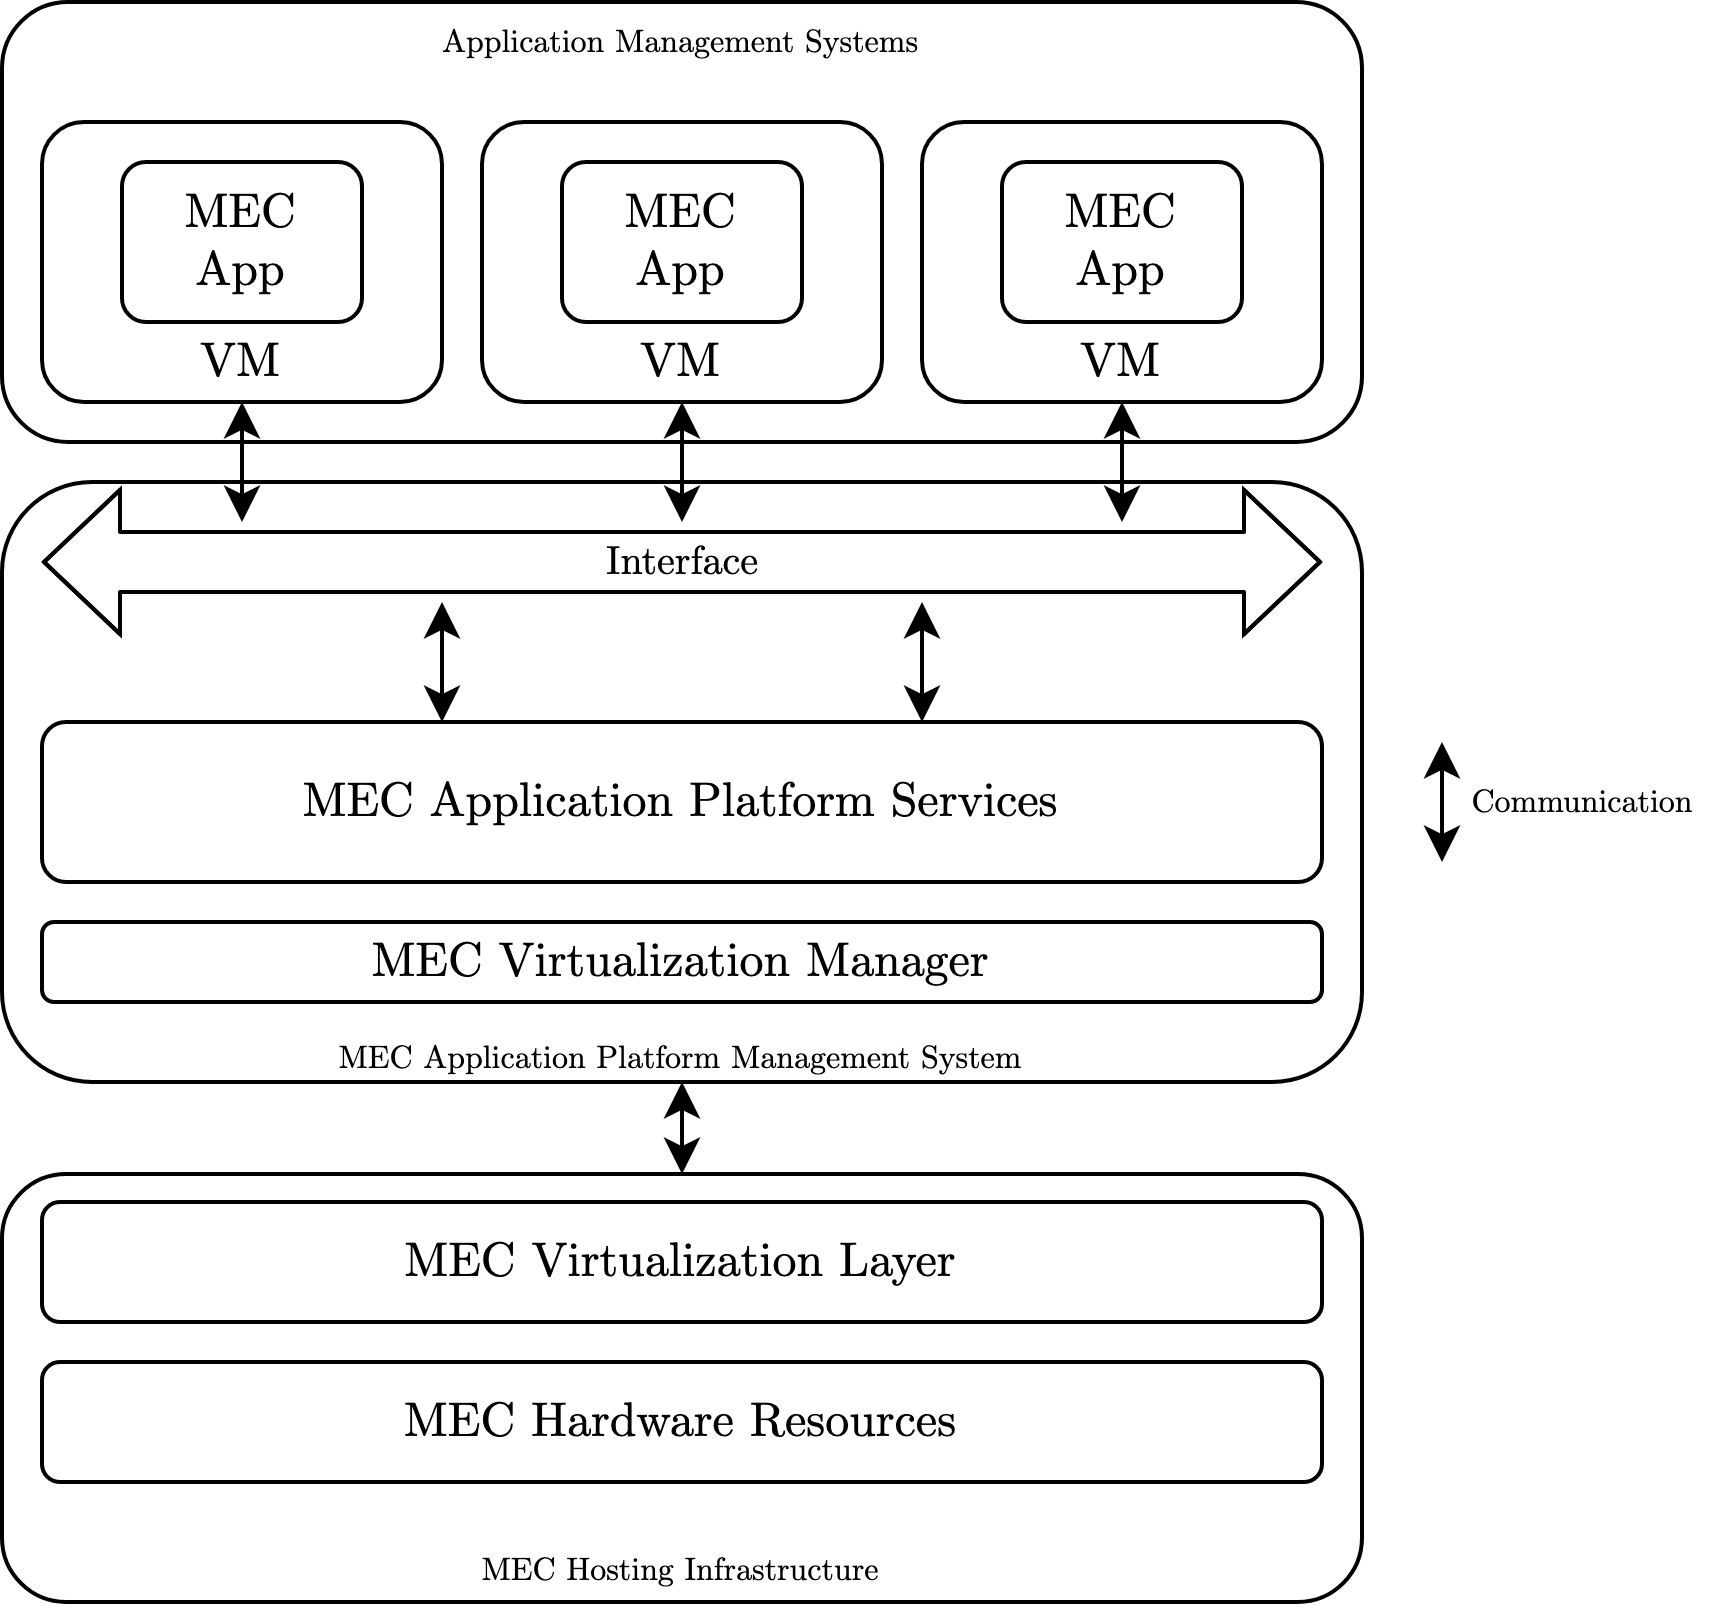
\includegraphics[scale=0.8]{chapters/architectures/figures/MEC_Server.png}
    \caption{Simplified version of the MEC Server architecture}
    \label{fig:MEC_Server}
\end{figure}

%TODO? snakke om NFV og SDN
\subsection{Network Functions Virtualization}
Network Functions Virtualization(NFV) is used in many MEC implementations\cite{patel_mec_nodate}. Networks need to run DNS, Firewall, NAT, etc to be able to run a modern network. Traditionally all of these functions have their own hardware. However, this makes infrastructure expensive, and hard to scale. NFV was introduced as a way to virtualize these functions. These functions then run on programmable switches and servers. Since they are easily controlled they are more scalable and flexible. The flexibility opens up for more possible architectures that can be deployed. For example, if we need to add extra MEC servers, instead of having extra off all the other server, it will just run through the NFV hardware, which then will take care of all the networking functions it needs. We can then easily send data to the new MEC server instead.

\subsection{Software-Defined Networking}
Software-Defined Networking(SDN) is often used together with NFV. Instead of having limiting the data layer to the hardware of switches, we run a VM on some hardware that lets networking be programmable. We can then set up rules and define were each packet should go. Since the network is now easily programmable, we can let the programmers take control of how the network is configured. The programmers can then change configuration on the fly, and therefore adapt the network to the context needed.
% In our experiments, the Emerald VM will consist of the two bottom systems, and we will focus on the application layer.

%TODO talk about HOW it is decided how much should be offloaded
\subsection{Offloading}
TODO

%SDN er at vi har virtuelle nettverk. Slik som at vi har eget nettverk i AWS på jobben. Vi kan da definere virtuelle nettverksdrivere og interfaces osv. For eksempel ha et eget virtuellt nettverk til kun databaseting.
%https://www.cisco.com/c/en/us/solutions/software-defined-networking/sdn-vs-nfv.html

% NFV og SDN er veldig like. NFV kjører en hel VM for å kontrollere nettverket. SDN kjører bare software og består som regel kun av rules på hva pakker skal og kan gjøre.


% sjekk ut 22?, 122,121?, 161, 163
% 162!! NFV (Network Function Virtualization)
% 166 SDN(software defined networking og NFV )
% 175, 176 ICN(Information centric networking)
% 164 NFV MEC architecture for video, gaming and AR

% IN MEC we do some on the mobile and some on the MEC server. Cloudlet however, aims to do as much as possible on the server.


% ------------------------------------------------------------------------------------------

\section{Cloudlet} \label{cloudlet} 
Satyanarayanan et al., proposed in their paper “The Case for VM-Based Cloudlets in Mobile Computing”\cite{satyanarayanan_case_2009} a solution to resource poverty of mobile devices and for the high latency in the Wide-Area Network(WAN). They wanted something that could fulfill the need for real-time responsiveness by having low-latency, one-hop, high-bandwidth access to a nearby \textit{Cloudlet}. They describe Cloudlets as a "data centre in a box"\cite{satyanarayanan_case_2009}. They are small computers that will run locally at each location where they are needed. All it needs is access to internet and power. An example is setting it up in a coffee shop. There it will be able to serve costumers with computation and storage if needed. All the coffee shop needs to do is plug in and configure the cloudlet. Since it is a relatively small box, it will not take much space or be in the way of costumers or employees. Having the Cloudlet so close, will help the response time stay low, as well as being predictable.

In this architecture, they focus on having as much as possible of the computation done on the nearby Cloudlet. The mobile device is just a thin client, and offloads all computation to the Cloudlet. If no Cloudlet is available, then the mobile device will try to offload to the distant cloud, or if all else fails, use its own computing power. This will heavily affect performance, especially if it has to do the work locally. However, if it detects a nearby Cloudlet, it can easily migrate the work over to it, and return to full functionality.
 
\begin{figure}[t]
    \centering
    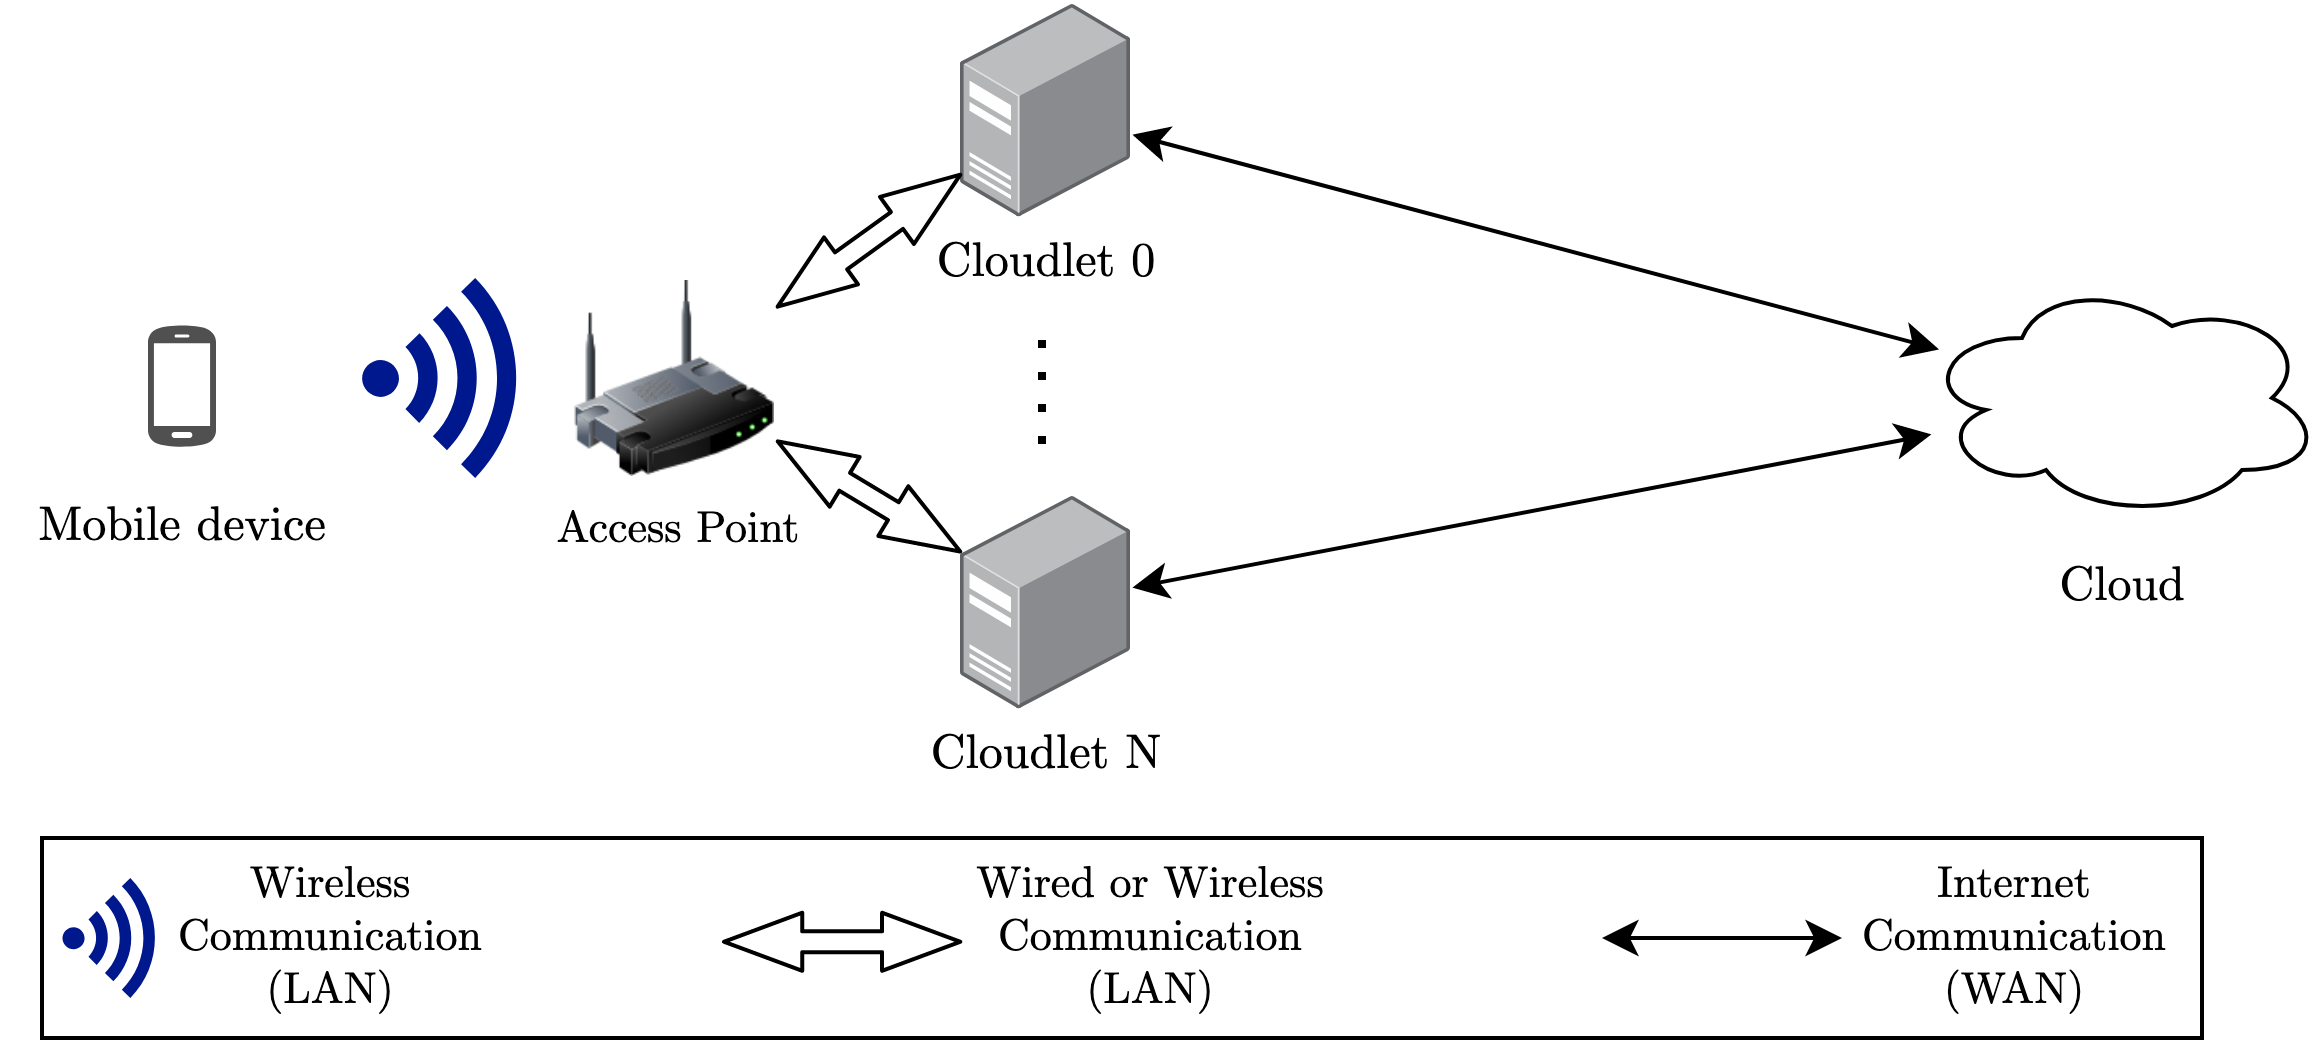
\includegraphics[scale=0.9]{chapters/architectures/figures/Cloudlet.png}
    \caption{Illustration of a simple Cloudlet connection}
    \label{fig:Cloudlet}
\end{figure}

% Husk at cloudlet kan videre overføre til distant cloud.
Figure \ref{fig:Cloudlet} shows a simple overview of how Cloudlets are connected. A mobile device will use WiFi or cellular to connect to its closest access point. The access point is further conneted to one or more Cloudlets with a LAN connection. Since they are so close in proximity of the mobile device, and on LAN, it can easily achieve just 1ms round-trip-time to the Cloudlet. In their paper, Satyanarayanan et al.\cite{satyanarayanan_case_2009} also proposes that that ideally, the Cloudlets them selves can be the access point, such that the Cloudlet is truly one-hop away, and so that they become more ubiquitous. The mobile device is usually connected to just one Cloudlet, but can easily be connected to several if needed. The Cloudlets are further connected to the distant cloud. Not shown in the figure is the case when there is no Cloudlets available. It will then connect directly to the Cloud instead of via a Cloudlet. 


\subsection{Offloading}
To simplify deployment, Cloudlets use \textit{transient customization of Cloudlet infrastructure}. Ideally it should be self managing, but it is never that easy. They want to use VMs that are fast and easy to deploy on the Cloudlets. Each time a mobile device wants to use a Cloudlet, it will send a small overhead to the server that contains enough information to start a VM that can be use to offload the work. By using VMs they ensure that creating programs for the Cloudlet is not limited to an small API or language. In other words, they let the developers decide the environment. The Cloudlet will get rid of the VM after it is finished with its use. This ensures that the Cloudlet is in the same state as before it was used.



% ------------------------------------------------------------------------------------------


\section{Content Delivery Networks}
Content Delivery Networks(CDN) are providers that have focused on putting servers close to the users. Firms like Akamai will have deals with local Internet Service Providers (ISP) to have some servers at their facilities. This ensures that their servers are only a few hops away from the clients. You also have technologies like Google AMP, which lets you have cached stripped down versions of websites cached at these CDNs to help speed up website loading.
%Diagram med servere som ligger hos ISP, og servere som ligger langt unna. Tenk på Netflix først prøve og hente ved ISP før den går videre til frankfurt eller amerika.



\section{Google Anthos}
% Uses devices in your home like the chromecast or google home?
%% bare skriv om en av de fog computing arkitekturene så er du i gang! :D

\section{Fog Computing for Big Data}
%https://dl.acm.org/doi/pdf/10.1145/2818869.2818898

% TODO:

% Odessa
% MAUI

% peer to peer?

% MCC vs MEC


\section{Summary}

\chapter{Implementation}\label{chapter:implementation}
In this chapter we will show how we have implemented the architectures presented in chapter \ref{chapter:architectures}.

\section{Testing Programs}
We have developed an application for testing computation offloading. It is easily configurable and flexible for testing. The next two subsections will show how it is implemented.

\subsection{Computation offloading}
For computation offloading we initially wanted to implement Eratosthenes Sieve for finding primes. This is because it has an interesting way parallelizing, and therefore distributing the work. However, due to an limitation from the Emerald VM, memory runs out when trying to find primes higher than a million. Memory use of the algorithm can be optimized, but it does not change the fact that Eratosthenes Sieve is a memory intensive algorithm. Therefore we are doing hashing instead. Hashing is a low memory, compute intensive task. This is excellent for our simulation as we primarily want to focus on computational use and latency.






\subsection{Classes and structure}
\begin{figure}[t]
    \centering
    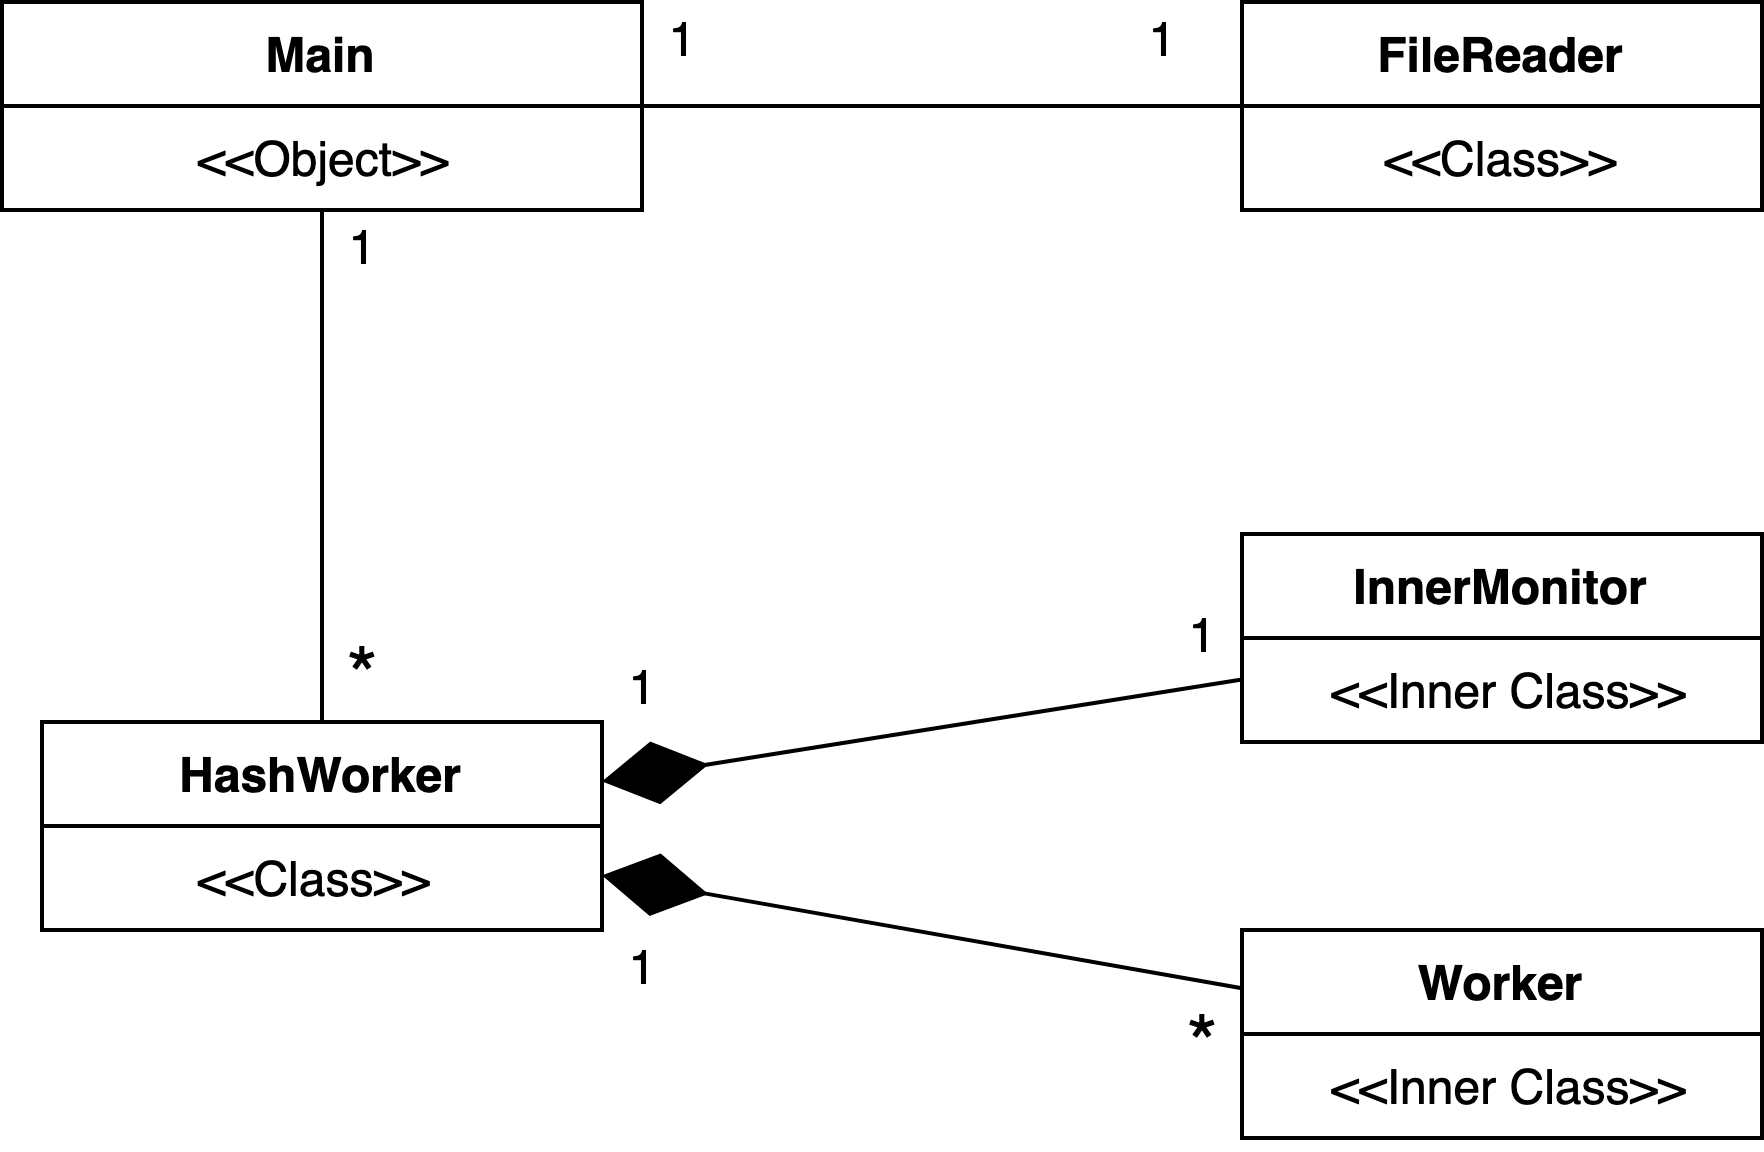
\includegraphics[scale=0.9]{chapters/implementation/figures/HashWorker_class_diagram.png}
    \caption{Illustration of the class structure used for computation offloading}
    \label{fig:HashWorker_class_diagram}
\end{figure}
Figure \ref{fig:HashWorker_class_diagram} shows the class structure. We have four classes and one object. We will now go through each of them and briefly explain what they do.


%Mention that since InternalMonitor has fields, getters and setters are automatically created at compile time, and since it is in a monitor, it is guaranteed that only one thread at a time can call those functions. 


\subsubsection{FileReader}
Below is the interface of class FileReader:
\begin{lstlisting}[language=emerald]
const FileReader <- class FileReader
  export op readFile[fileName: String] 
                            -> [res: Array.of[String]]
                            
  export function convertConfigToIntegers
                            [input: Array.of[String]] 
                          -> [res: Array.of[Integer]]
                            
  function stripLast[i: String] -> [o: String]
end FileReader
\end{lstlisting}
The operation \verb|readFile| will read the file with the path provided in parameter \verb|fileName|. For each line it reads, it will delete the last character with \verb|stripLast|, as it is a unwanted newline character. The function \verb|convertConfigToIntegers| is a function that converts an array of strings to an array of integers. This is needed because configs consists of lines of numbers, but they are read as strings.



\subsubsection{HashWorker}
Below is the interface of class HashWorker:
\begin{lstlisting}[language=emerald]
const HashWorker <- class HashWorker
                                [limitation: Integer]
  
  attached const workload %String

  attached const mon <- InnerMonitor.create

  attached const InnerMonitor 
                        <- monitor class InnerMonitor

  attached const Worker
                  <- class Worker[iterations: Integer]

  initially

  export op setLimitation[lim: Integer]
  
  export op doWork[iterations: Integer, 
                    work: LocalWorkload, 
                    frequencyOfGet: integer]

  export op collectTimeUsed -> [res: Time]
end HashWorker
\end{lstlisting}
HashWorker is an object that is distributed to all machines. The role of HashWorker is to provide an interface for main to start and control work. The constant \verb|mon| is used to store an instance of the \verb|InnerMonitor| class. Then we have the definitions for \verb|InnerMontor| and \verb|Worker|. They are defined inside the HashWorker class and are therefore inner classes. Then we have the \verb|initially| section. Here we ensure that the class parameter \verb|limitation| is equal to or higher than zero. This is because the limitation is used to make a time constraint, and we don´t want negative time. Operation \verb|setLimitation| is there to be able to change the limitation during runtime. Operation \verb|doWork| will create an instance of the \verb|Worker| class. It takes a parameter \verb|iterations| which is how many iterations we want the node to do, \verb|work| which is the workload that the worker will hash, and \verb|frequencyOfGet| which is how often we retrieve information from Local (the mobile device). Operation \verb|collectTimeUsed| is used to collect the time used after process is done. When called, it will wait for the process in Worker to be done, then return the time used.
Notice that all of the constants are attached. This is because we want to ensure that all of them are on the same node as the HashWorker instance. This reduces the amount of costly remote reads.




\subsubsection{InternalMonitor}
Below is the whole class of InnerMontor:
\begin{lstlisting}[language=emerald]
attached const InnerMonitor 
                        <- monitor class InnerMonitor
  field waiting : Boolean <- true

  field timeTaken : Time <- nil
end InnerMonitor
\end{lstlisting}
As discussed in section \ref{emerald:field}, fields in Emerald automatically generates getters and setters. Since it is in a monitor class it is guaranteed that invoking them is mutual exclusive. In other words, the getters and setters that are automatically created within the class is safe to use in parallel. Variable \verb|timeTaken| is used to store the time used by the process in class \verb|Worker|. Variable \verb|waiting| is used to ensure that main does not collect \verb|timeTaken| before the worker is done. 





\subsubsection{Worker}
Below is the skeleton of class Worker.

\begin{minipage}{\linewidth}
\begin{lstlisting}[language=emerald]
attached const Worker 
                <- class Worker[iterations: Integer]
                
    initially
    
    process
    
    function djb2Hash[str: String] -> [res: Integer]
end Worker
\end{lstlisting}
\end{minipage}
The \verb|initially| section will assert that iterations are higher than zero, because we should avoid doing negative amount of work. The \verb|process| section is where the actual work of the node happens. When \verb|doWork| is called in class \verb|HashWorker|, it creates an instance of the Worker class by invoking operation \verb|create|. The process is then started. In the process, it will run parameter \verb|iterations| number of iterations. The hashing algorithm we use is called \textit{Djb2}. Our implementation is a converted version from a C implementation found here\cite{noauthor_hash_nodate}. 
\begin{lstlisting}[language=emerald]
function djb2Hash[str: String] -> [res: Integer]
  res <- 5381
  for i : Integer <- 0 while i < str.length 
                                    by i <- i + 1
    res <- res * 33 * str[i].ord
  end for
end djb2Hash
\end{lstlisting}
The algorithm takes a string, iterates over it and multiplies itself with 33 and the characters ordinal number. To make it even more compute heacy, we convert the result to string, and then re-insert that into the hash function 10000 times. We see that as one iteration, as shown in figure \ref{fig:Hashing_algorithm_iteration}. In other words, the HashWorker will do what figure \ref{fig:Hashing_algorithm_iteration} shows, parameter \verb|iterations| number of times. Since we just throw out the result after each time, Emeralds garbage compiler will ensure that we have plenty of memory available. 
\begin{figure}[t]
    \centering
    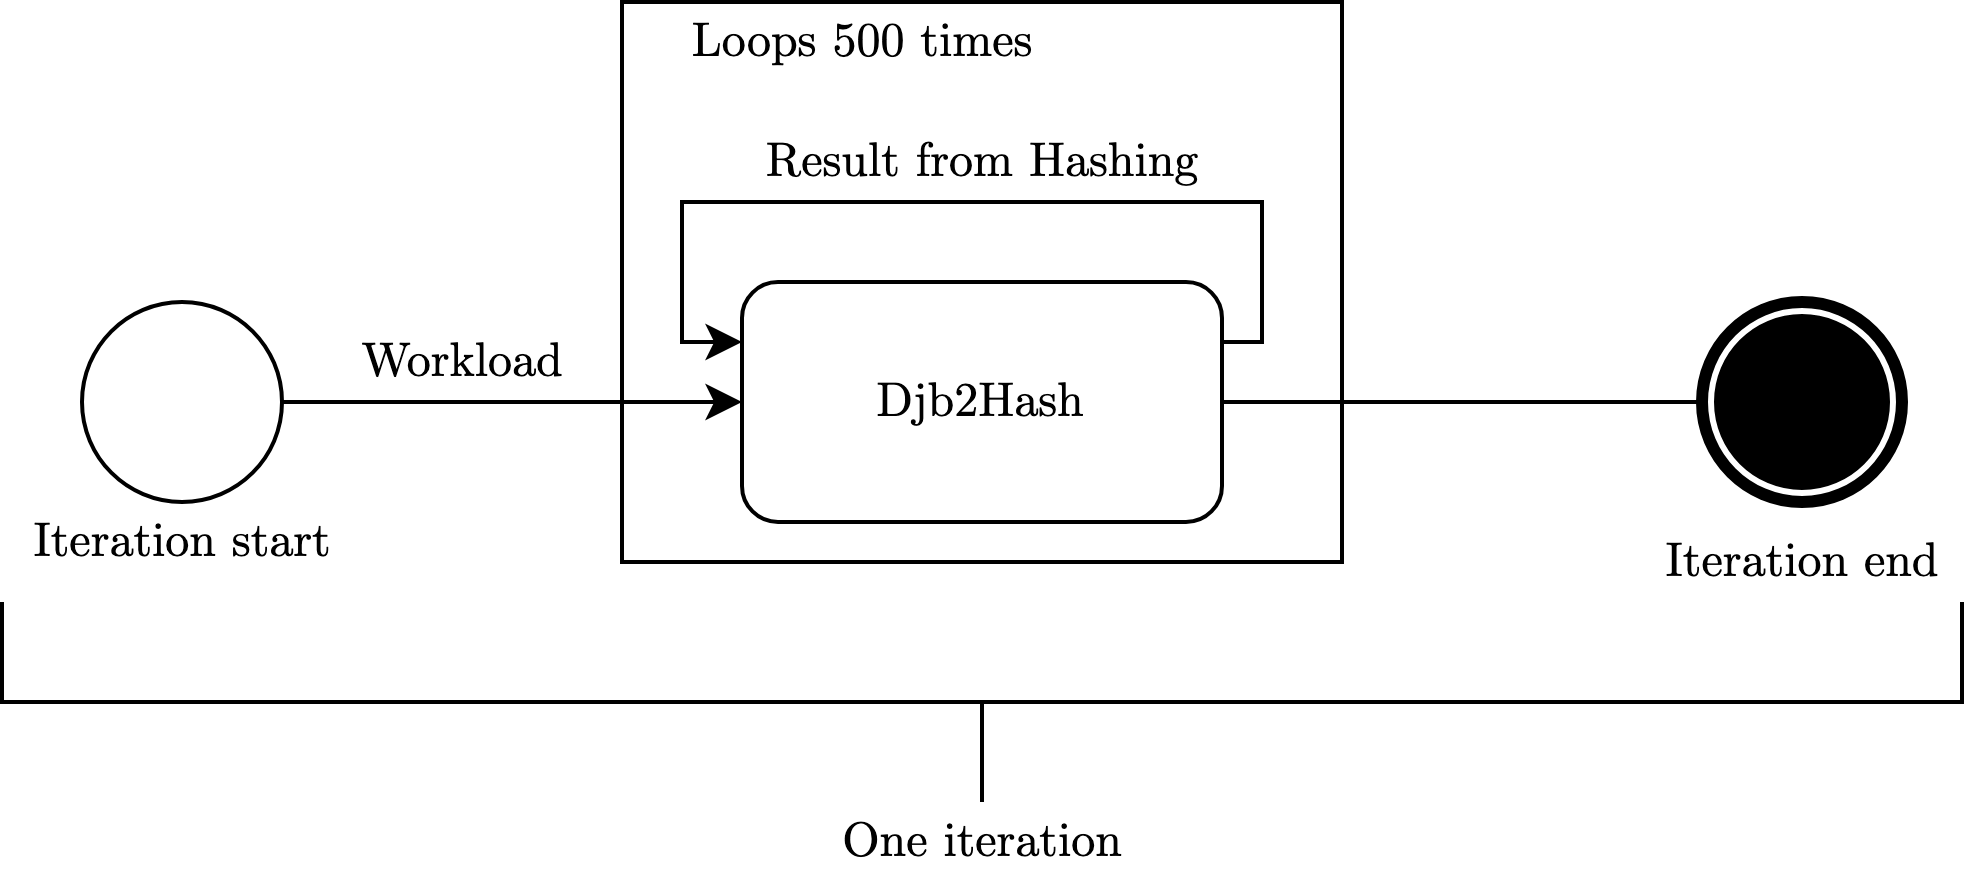
\includegraphics[scale=0.9]{chapters/implementation/figures/Iteration.png}
    \caption{Illustration of one iteration in the HashWorker}
    \label{fig:Hashing_algorithm_iteration}
\end{figure}
In each iteration it will also check if we have to get information from Local, as well as taking the time on how long we do calculations and how long we wait for response.



\subsubsection{Main}
Main only has an initially section that will do a number of steps. First it will move through all nodes and print some information on each node. This is mainly for debugging, and to ensure that things are running correctly. Further it will invoke the create an instance of the \verb|FileReader| class and read config file that you have specified. Config files are discussed in subsection \ref{subsection:configfiles}. Further, it will use this config to initilize \verb|HashWorker| instances and move them to a node decided by user input. Then, it will iterate through all \verb|HashWorker| instances and invoke operation \verb|doWork|. All processes should then have started. Finally, it will collect and print the results.



\subsection{Simulating CPU restrictions}
To simulate CPU restrictions, we place a limitation on each HashWorker. To be able to accurately control how much work is done on each HashWorker, we have implemented a way of specifying how many iterations (see figure \ref{fig:Hashing_algorithm_iteration}) each node can do per second.



\subsection{Config files}\label{subsection:configfiles}
When the \verb|FileReader| class reads in the config file, it expects a very simple syntax. Each line should be a positive integer. For example a file that for two HashWorkers will set their limitations to 0 and 100 and make them both do 50 iterations, and make them get from Local with a frequency of 1 and 30 iterations, will look like this:
\begin{lstlisting}
0
100
1
30
50
50

\end{lstlisting}
The \verb|FileReader| reads each line until the newline character. The config file is terminated by an emtpy line at the end. After everything is read, it will convert them to an array of Integers, instead of array of Strings.

\subsection{Placing HashWorkers}
Placement of HashWorkers is prompted in the terminal. When testing you will get information about an HashWorker, and a choice for which node you want to place it on. 














% -----------------------------------------------------------------------------------

\section{Multi-Access Edge Computing}

\begin{figure}[t]
    \centering
    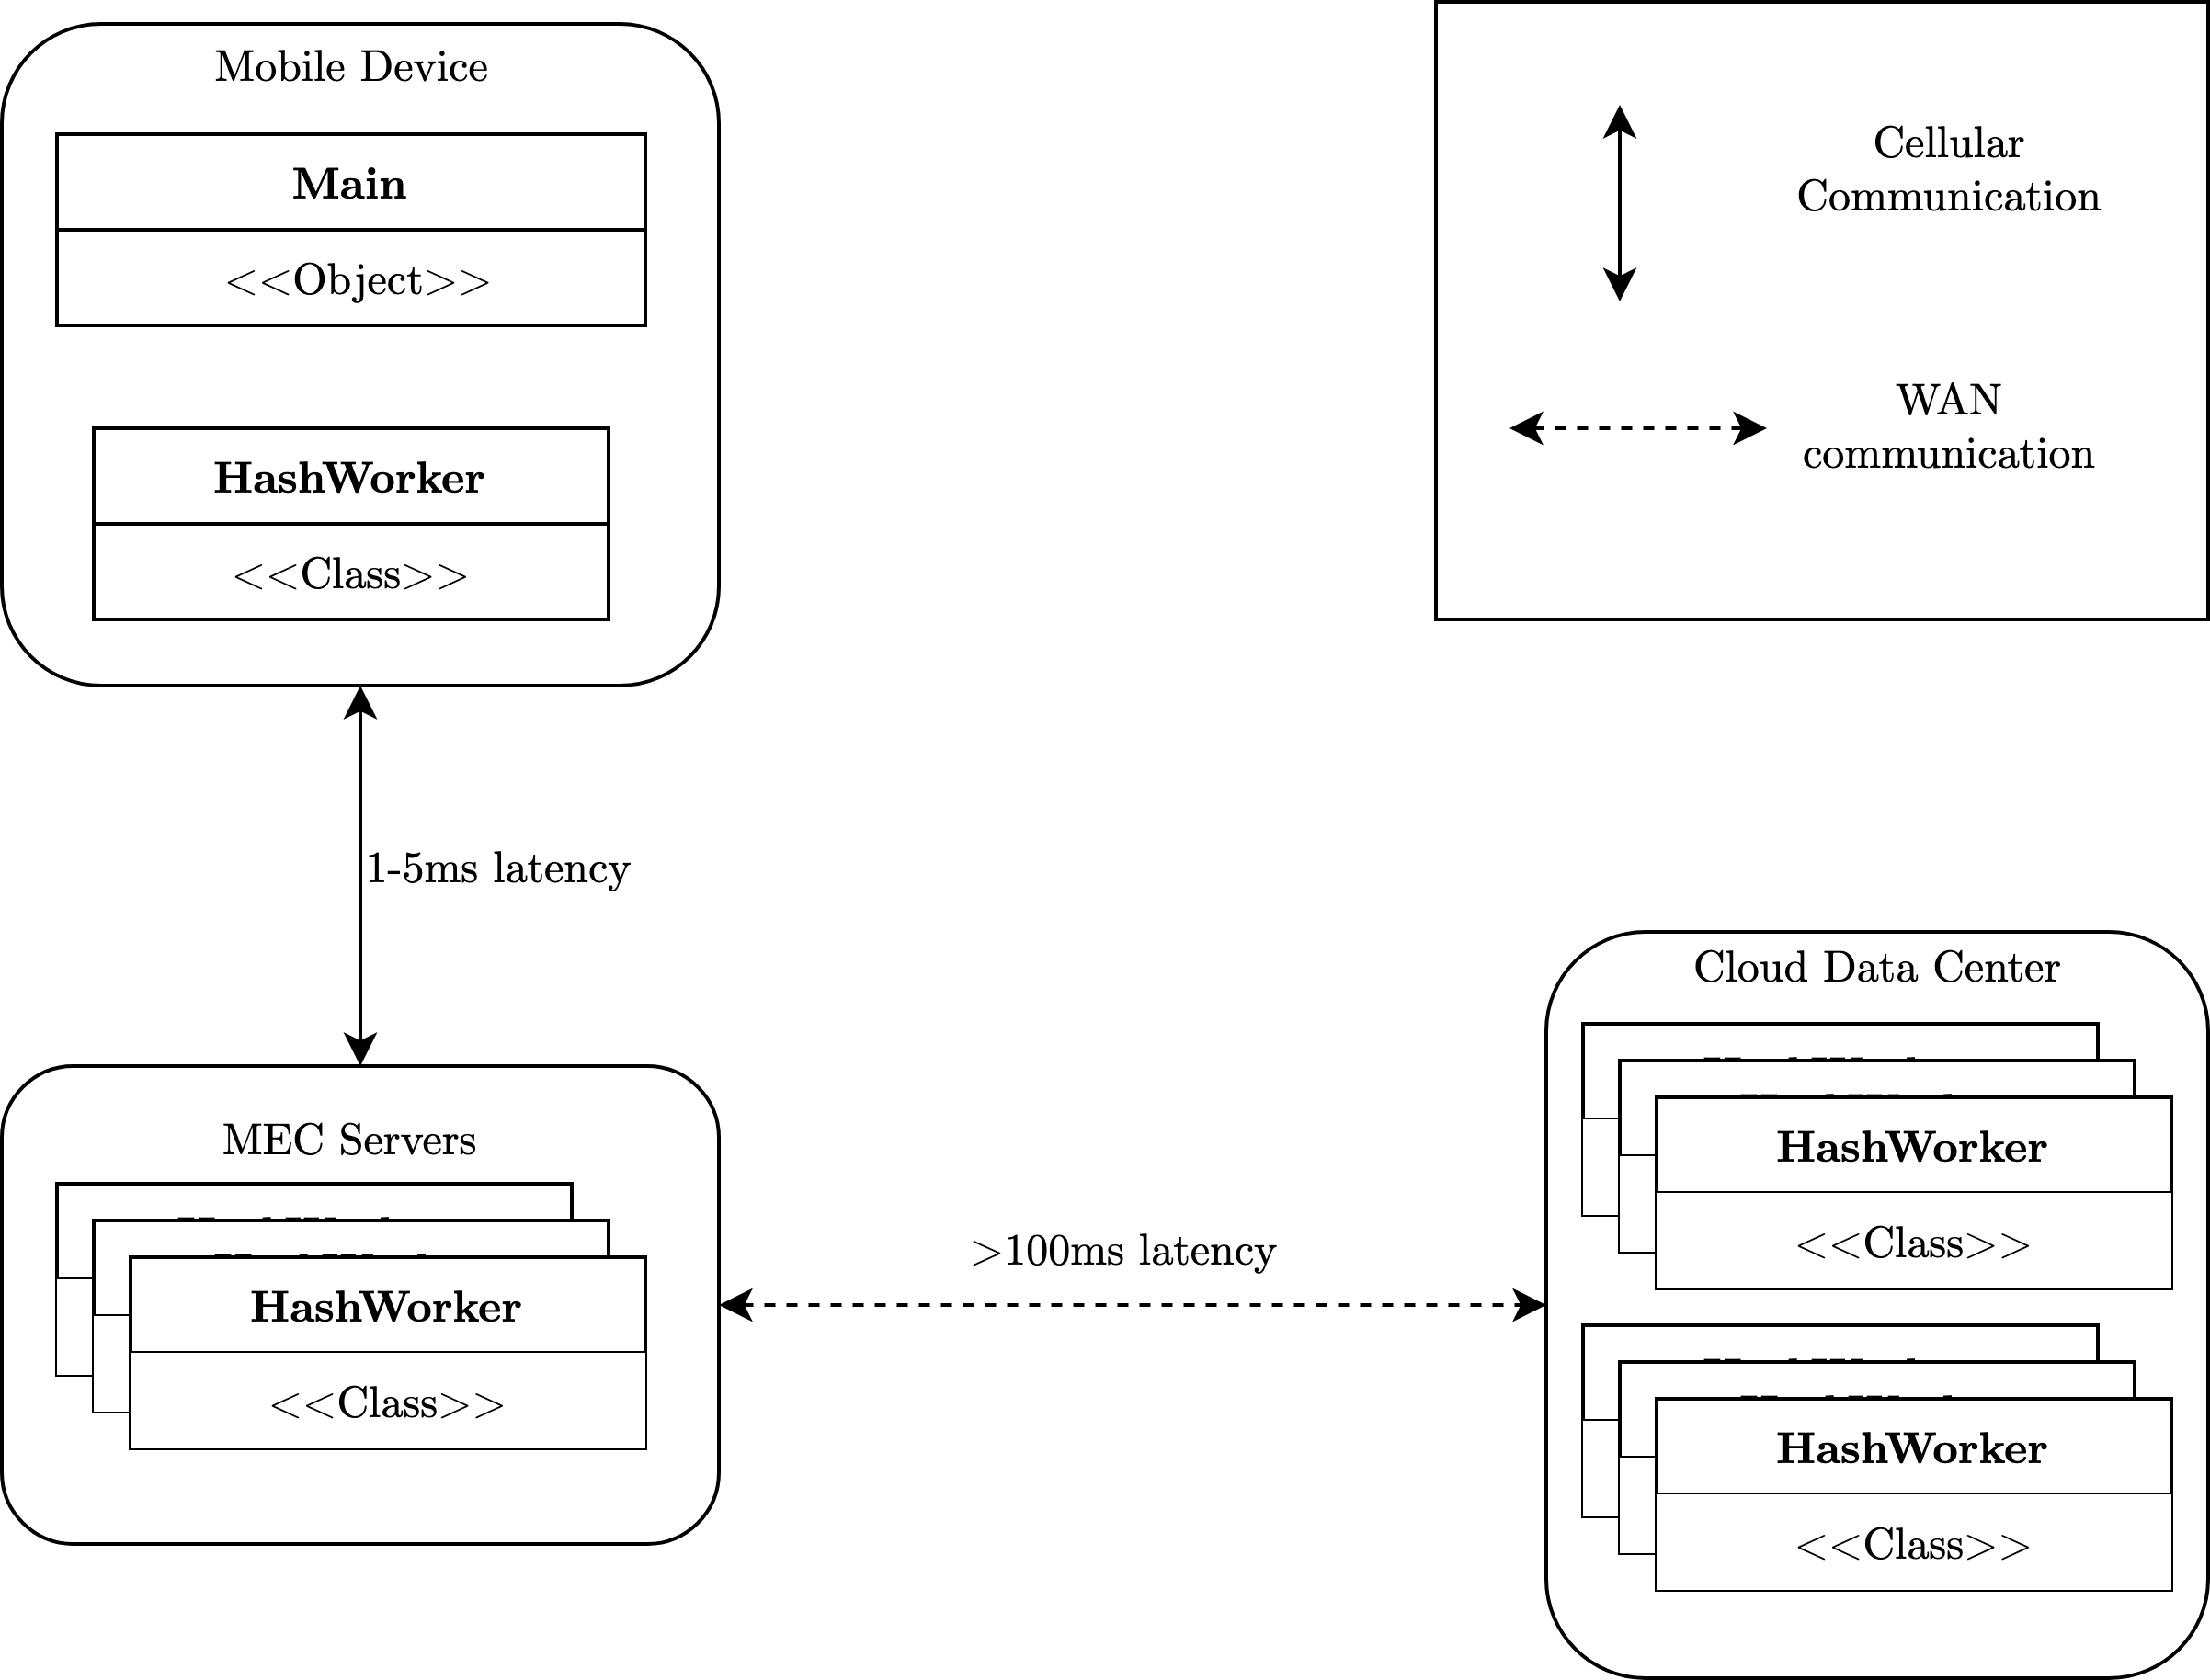
\includegraphics[scale=1]{chapters/implementation/figures/MEC_implementation.png}
    \caption{Illustration of the node structure used for computation offloading in MEC}
    \label{fig:MEC_implementation}
\end{figure}
Figure \ref{fig:MEC_implementation} illustrates how three nodes can be set up. The \verb|Main| object will reside on the mobile device, as that is where we want the result. We can create several HashWorkers to place them on servers. However, the Cloud Data Center will have enough resources to have significantly more HashWorkers than the MEC Servers, and the MEC Servers can have significantly more HashWorkers than the mobile client. The MEC Servers can consist of one or more machines that hosts one to many HashWorker instances. The Cloud Data Center consists of many machines that can host one to many HashWorker instances.




% -------------------------------------------------------------------

\section{Cloudlets}
\begin{figure}[t]
    \centering
    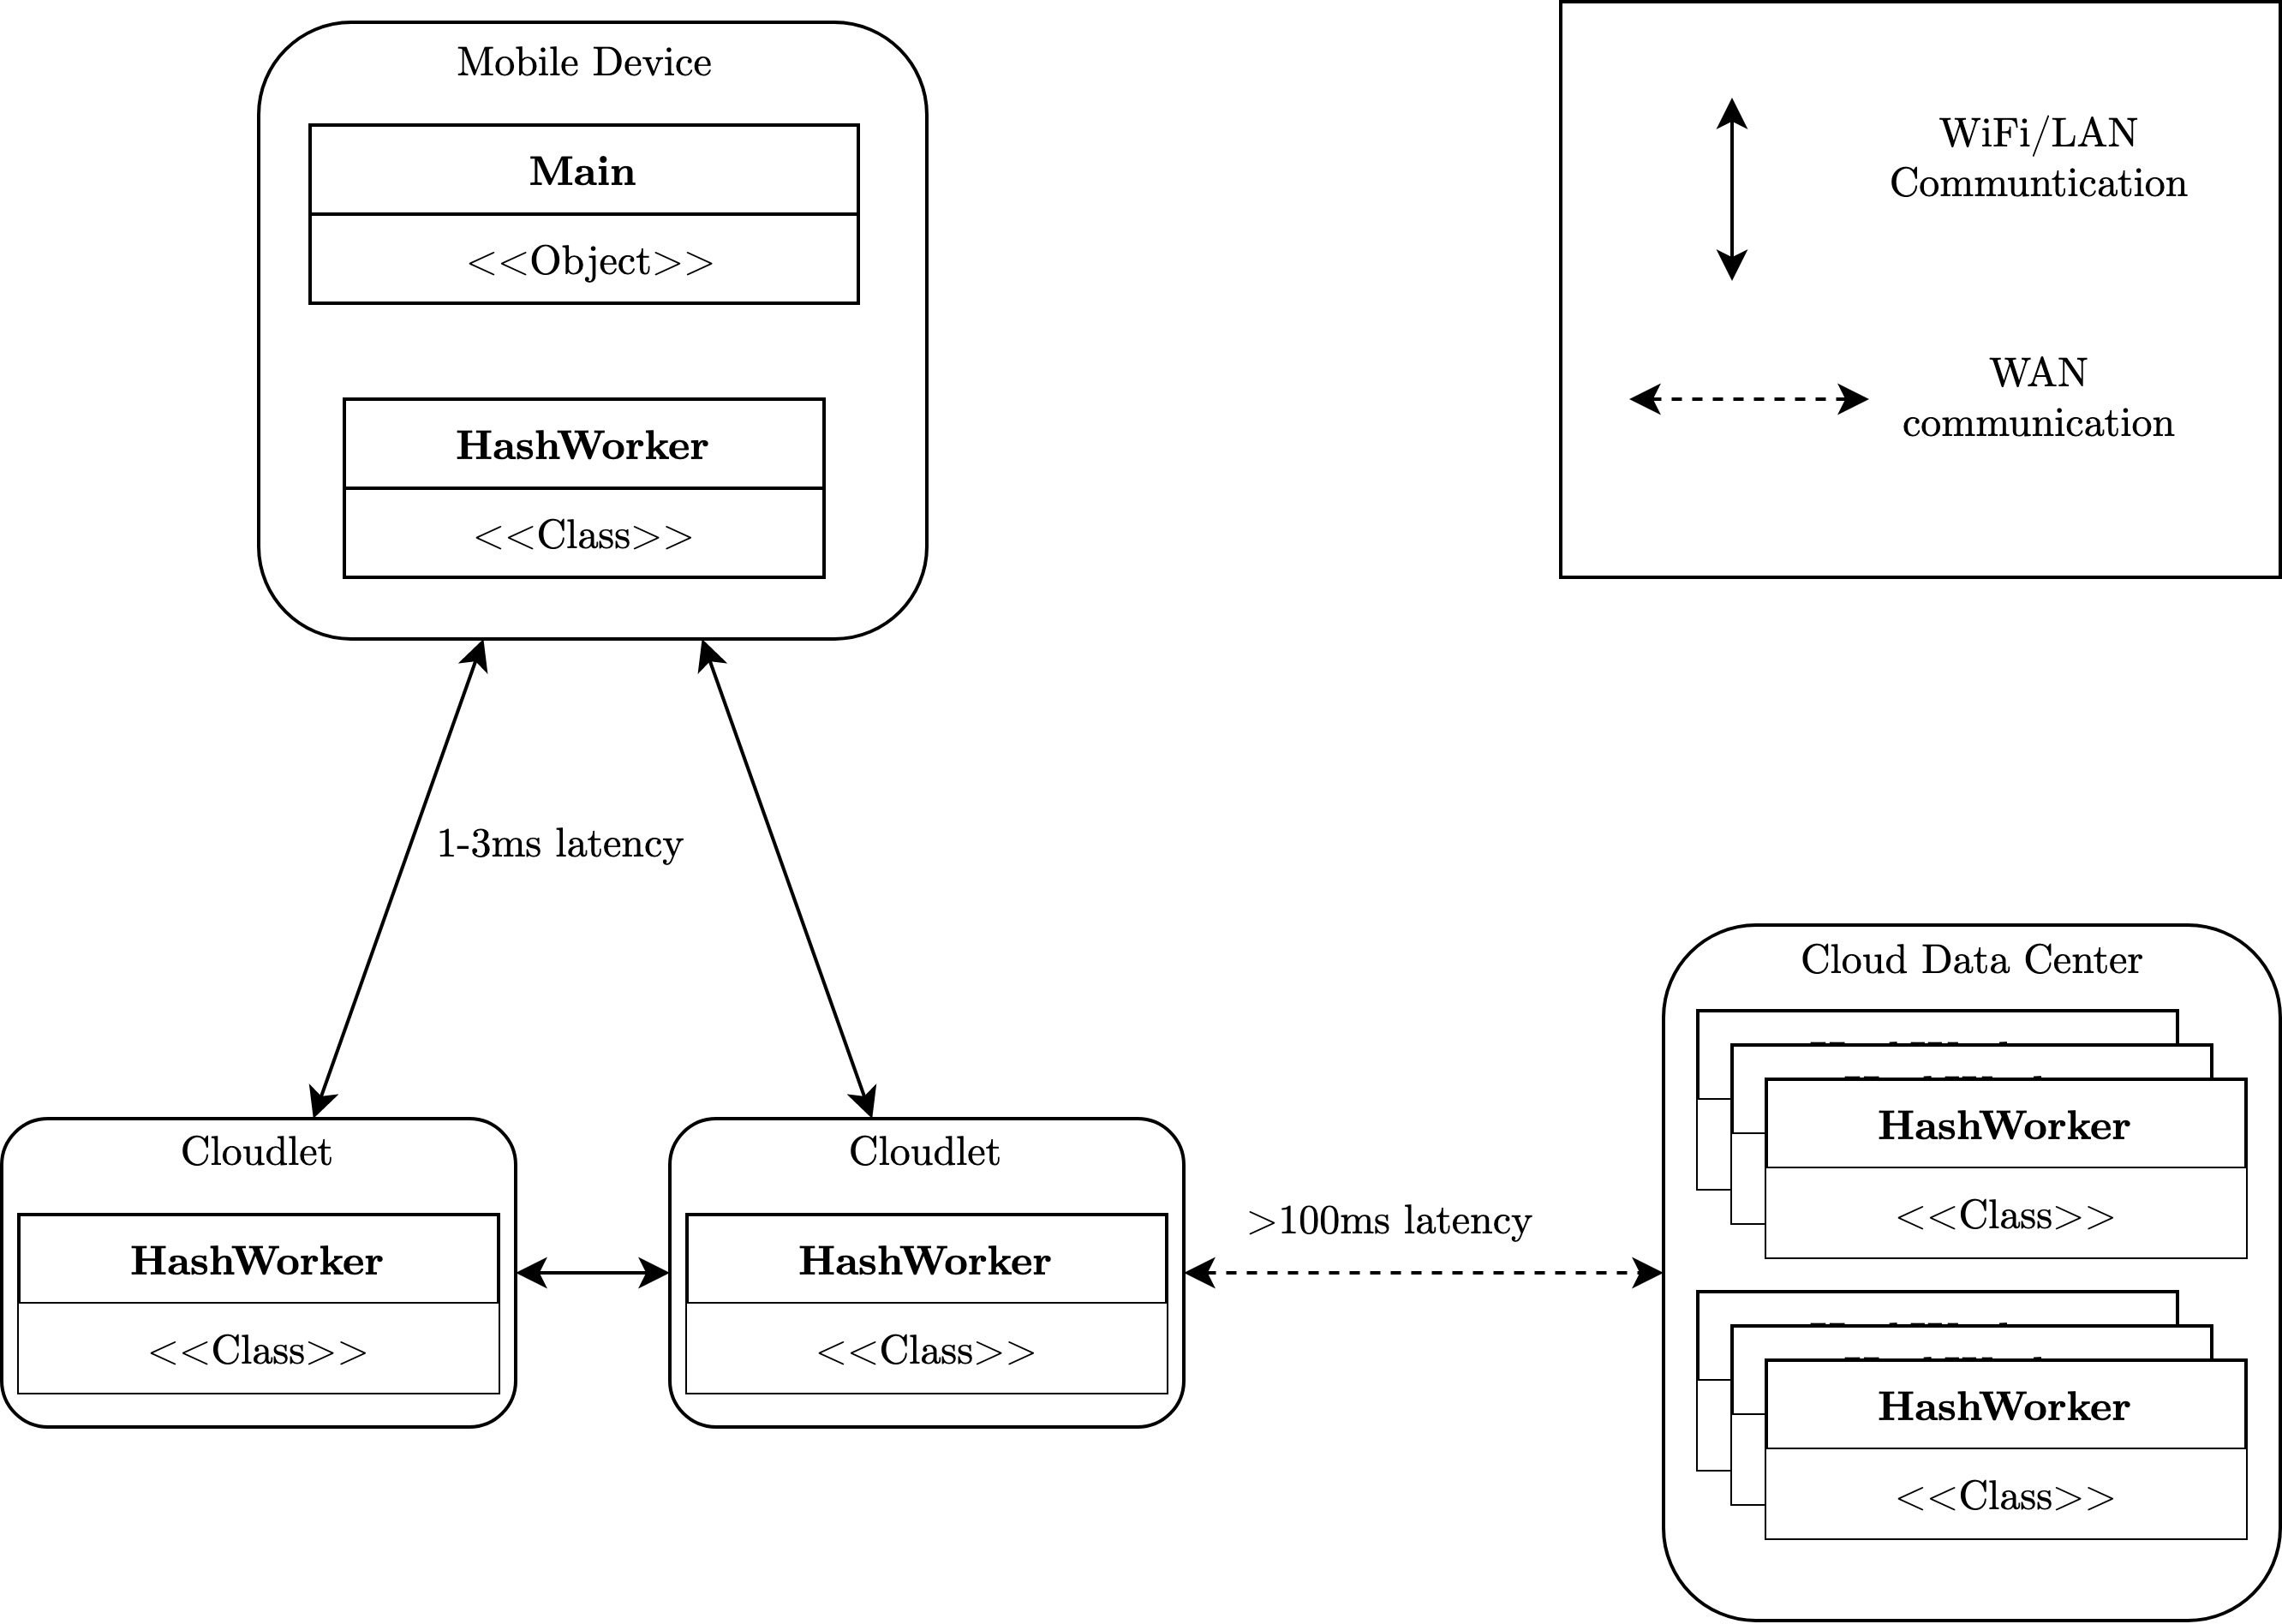
\includegraphics[scale=0.9]{chapters/implementation/figures/Cloudlet_implementation.png}
    \caption{Illustration of the node structure used for computation offloading with Cloudlets}
    \label{fig:Cloudlet_implementation}
\end{figure}
Figure \ref{fig:Cloudlet_implementation} illustrates how we can set up an example implementation of Cloudlets. The mobile device will be in very short distance of the Cloudlets and therefore use WiFi to connect with them. In our tests, the Cloudlets are not access points themselves, and therefore there is a WiFi accesspoint hop between the mobile device and the Cloudlets.










\section{Summary}
In this chapter we have described the prototype we have created. The prototype can easily be setup with configuration files to control different parameters for each worker on each node. This lets us easily set up high-level simulations of Near-Far architectures and models. Additionally we have provided some examples of how you can use it to model Cloudlets and Mobile Edge Computing.


\chapter{Evaluation}\label{chapter:evaluation}
In this chapter we will evaluate the architectures described in chapter \ref{chapter:architectures} with the method described in chapter \ref{chapter:design_of_experiments}. Some of them will additionally be evaluated with the implementation from chapter \ref{chapter:implementation}.






\section{Assumptions}
\subsection{Bandwidth}
When evaluating we are making some assumptions about bandwidth. Table \ref{tab:Bandwidth_latency} shows latency and bandwidth for different technologies. The WiFi bandwidths are based on data from CenturyLink\cite{noauthor_24_nodate}. The 4G and 5G bandwidths are real-world examples from 4g.co.uk\cite{noauthor_how_nodate}. The 4G latency are from ping tests, while the 5G latency are from Verizon\cite{noauthor_what_2020}.

\begin{table}[h!]
    \centering
    \begin{tabular}[c]{|c|c|c|}
        \hline
        Technology & Latency (ms) & Bandwidth (Mbps) \\
            &   &  Download/Upload \\
        \hline
        \hline
        Wifi (2.4GHz) & <=1 & 150/150  \\
        \hline
        Wifi (5GHz) & <=1 & 450/450  \\
        \hline
        4G & 30-65 & 42/25  \\
        \hline
        5G & 30 & 200/100  \\
        \hline
        Wired LAN & <=1 & 1000+  \\
        \hline
        WAN & 10-300+ & 1000+  \\
        \hline
        
        
    \end{tabular}
    \caption{Latency and bandwidth for different technologies.}
    \label{tab:Bandwidth_latency}
\end{table}
When doing calculations in this chapter, we will be using numbers from table \ref{tab:Bandwidth_latency}.




\subsection{Hardware}
According to cpubenchmark\cite{noauthor_passmark_nodate}, flagship phones is about half as fast as a standard desktop CPU. We assume that we are dealing with below average CPU's cellphones, as most people do not have the flagship phone. We will test different strengths of the MEC Server. We assume that the data centre will have plenty of resources. In total, we want to do 10000 iterations spread over all the nodes.




\subsection{Local execution}
%lacking geographic location?
\begin{table}[h!]
    \centering
    \begin{tabular}[c]{|c|c|c|c|}
        \hline
        Node type & Limitation & Iterations & Time used (s) \\
        \hline
        \hline
        Local & 30 & 10000 & 333.6 \\
        \hline
    \end{tabular}
    \caption{Only local execution.}
    \label{tab:MEC_local_execution}
\end{table}
Table \ref{tab:MEC_local_execution} shows the time used for local execution only.


\subsection{Common results}
The tables shown in the following two sub subsections are common for both MEC and Cloudlets. This is because we test the same hardware, so when latency is not a factor, we will have the same results. They are all results of tests with little to no latency.

\subsubsection{Full offloading}
%spread out over more nodes
\begin{table}[h!]
    \centering
    \begin{tabular}[c]{|c|c|c|c|}
        \hline
        Node type & Limitation & Iterations & Time used (s)\\
        \hline
        \hline
        Local & 30 & 0 & 0 \\
        \hline
        Near & 100 & 2500 & 23.3 \\
        \hline
        Far & 300 & 7500 & 30.5 \\
        \hline
    \end{tabular}
    \caption{Full offloading.}
    \label{tab:MEC_full_offloading}
\end{table}

\begin{table}[h!]
    \centering
    \begin{tabular}[c]{|c|c|c|c|}
        \hline
        Node type & Limitation & Iterations & Time used (s)\\
        \hline
        \hline
        Local & 30 & 0 & 0 \\
        \hline
        Near & 100 & 2800 & 27.3 \\
        \hline
        Far & 300 & 7200 & 29.8 \\
        \hline
    \end{tabular}
    \caption{Full offloading with more balance.}
    \label{tab:MEC_full_offloading_balanced}
\end{table}

Table \ref{tab:MEC_full_offloading} and \ref{tab:MEC_full_offloading_balanced} shows time used when offloading work to nodes that have little to no latency from Local (less than 1 ms). This essentially shows how much time is used on calculation if we have no communication between nodes. 

\subsection{Partial offloading}
The tables shown in this subsection are common for both MEC and Cloudlets. This is because we test the same hardware, so when latency is not a factor, we will have the same results.
\begin{table}[h!]
    \centering
    \begin{tabular}[c]{|c|c|c|c|}
        \hline
        Node type & Limitation & Iterations & Time used (s)\\
        \hline
        \hline
        Local & 30 & 1000 & 33.0 \\
        \hline
        Near & 100 & 2000 & 19.5 \\
        \hline
        Far & 300 & 7000 & 30.6 \\
        \hline
    \end{tabular}
    \caption{Partial offloading.}
    \label{tab:MEC_partial_offloading}
\end{table}


\begin{table}[h!]
    \centering
    \begin{tabular}[c]{|c|c|c|c|}
        \hline
        Node type & Limitation & Iterations & Time used (s)\\
        \hline
        \hline
        Local & 30 & 850 & 28.1 \\
        \hline
        Near & 100 & 2700 & 26.5 \\
        \hline
        Far & 300 & 6450 & 29.1 \\
        \hline
    \end{tabular}
    \caption{Partial offloading with more balance.}
    \label{tab:MEC_partial_offloading_balanced}
\end{table}
Table \ref{tab:MEC_partial_offloading} and \ref{tab:MEC_partial_offloading_balanced} shows the result of offloading with less than 1 ms latency and little overhead.






\section{Multi-Access Edge Computing} \label{section:MEC_evaluation}

\subsection{Full offloading}
\begin{table}[h!]
    \centering
    \begin{tabular}[c]{|c|c|c|c|c|}
        \hline
        Node type & Limitation & Iterations & RTT to Local (ms)& Time used (s)\\
        \hline
        \hline
        Local & 30 & 0 & 0 & 0 \\
        \hline
        Near & 100 & 2800 & 30 & 92.8 \\
        \hline
        Far & 300 & 7200 & 170 & 1304.8 \\
        \hline
    \end{tabular}
    \caption{Full offloading with communication between Local and Near/Far.}
    \label{tab:MEC_full_offloading_latency}
\end{table}

Table \ref{tab:MEC_full_offloading_latency} shows how latency affects the work. Here, it will have to get data from Local after every iterations. There is a lot of communication between the nodes.

\begin{table}[h!]
    \centering
    \begin{tabular}[c]{|c|c|c|c|c|}
        \hline
        Node type & Limitation & Iterations & RTT to Local (ms)& Time used (s)\\
        \hline
        \hline
        Local & 30 & 0 & 0 & 0 \\
        \hline
        Near & 100 & 8500 & 30 & 279.3 \\
        \hline
        Far & 300 & 1500 & 170 & 267.9 \\
        \hline
    \end{tabular}
    \caption{Full offloading with communication and more balance in the nodes.}
    \label{tab:MEC_full_offloading_latency_balance}
\end{table}

Table \ref{tab:MEC_full_offloading_latency_balance} shows a more balanced workload distribution. The Near node is doing significantly more work. Here we also have to get data from Local after each iteration.














\subsection{Partial offloading}




\begin{table}[h!]
    \centering
    \begin{tabular}[c]{|c|c|c|c|c|}
        \hline
        Node type & Limitation & Iterations & RTT to Local (ms)& Time used (s)\\
        \hline
        \hline
        Local & 30 & 850 & 0 & 28.1 \\
        \hline
        Near & 100 & 2700 & 30 & 86.0 \\
        \hline
        Far & 300 & 6450 & 170 & 1131.2 \\
        \hline
    \end{tabular}
    \caption{Partial offloading with communication between Local and Near/Far.}
    \label{tab:MEC_partial_offloading_latency}
\end{table}

Table \ref{tab:MEC_partial_offloading_latency} shows how latency affects offloading. We have the same configuration as shown in table \ref{tab:MEC_partial_offloading_balanced}, but now the nodes are spread out and have latency affecting the offloading. The nodes have to get data from Local after each iteration.

\begin{table}[h!]
    \centering
    \begin{tabular}[c]{|c|c|c|c|c|}
        \hline
        Node type & Limitation & Iterations & RTT to Local (ms)& Time used (s)\\
        \hline
        \hline
        Local & 30 & 4550 & 0 & 151.3  \\
        \hline
        Near & 100 & 4525 & 30 & 149.8 \\
        \hline
        Far & 300 & 925 & 170 & 163.0 \\
        \hline
    \end{tabular}
    \caption{Partial offloading with communication and more balance in the nodes.}
    \label{tab:MEC_partial_offloading_latency_balance}
\end{table}


Table \ref{tab:MEC_full_offloading_latency_balance} shows a more balanced version. We can see that more of the work happens locally and on the node with less latency.

\subsection{Decreasing interaction}

\begin{figure}[t]
    \centering
    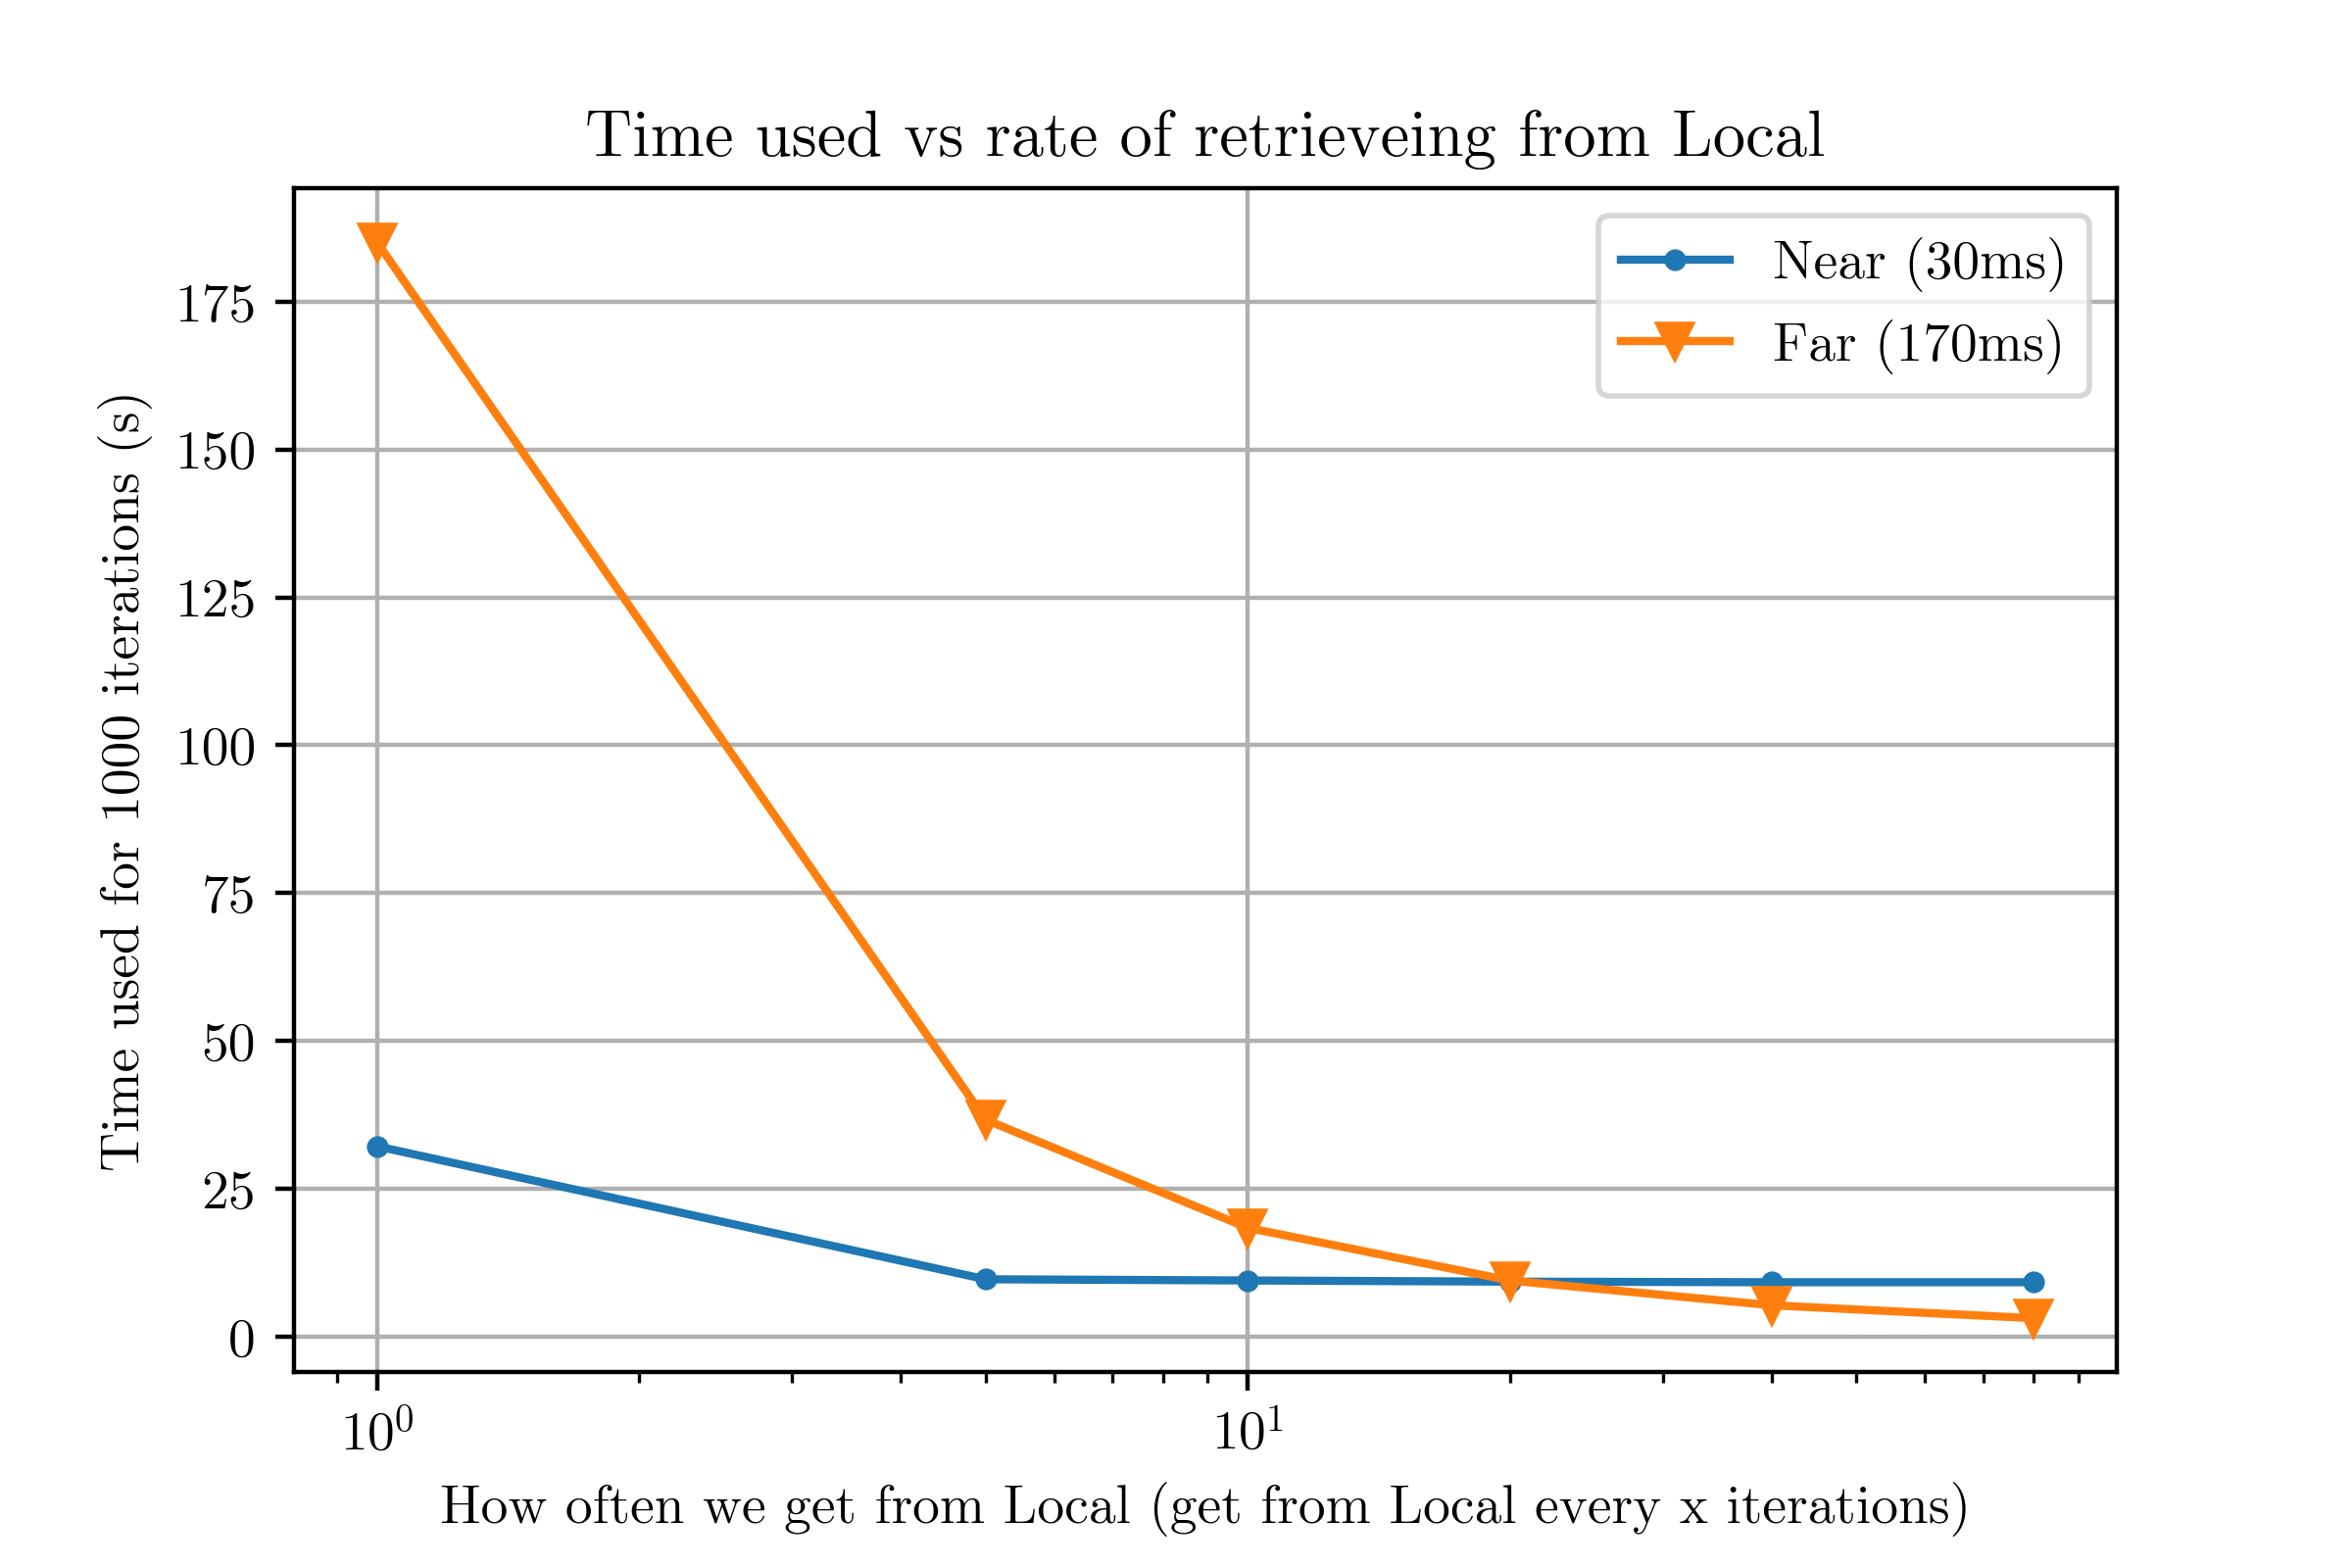
\includegraphics[scale=1]{chapters/evaluation/figures/times.png}
    \caption{Graph showing how interaction hurts. If x=10 then we get from Local every 10 iterations.}
    \label{fig:time_graph_near_far}
\end{figure}

Figure \ref{fig:time_graph_near_far} shows how latency affects the time used when you have to constantly get data from the Local device. We have tested with various frequencies of interaction. The graph essentially shows how much time is used on Near or Far node with regards to how often it has to get data from the Local node. 
\begin{figure}[t]
    \centering
    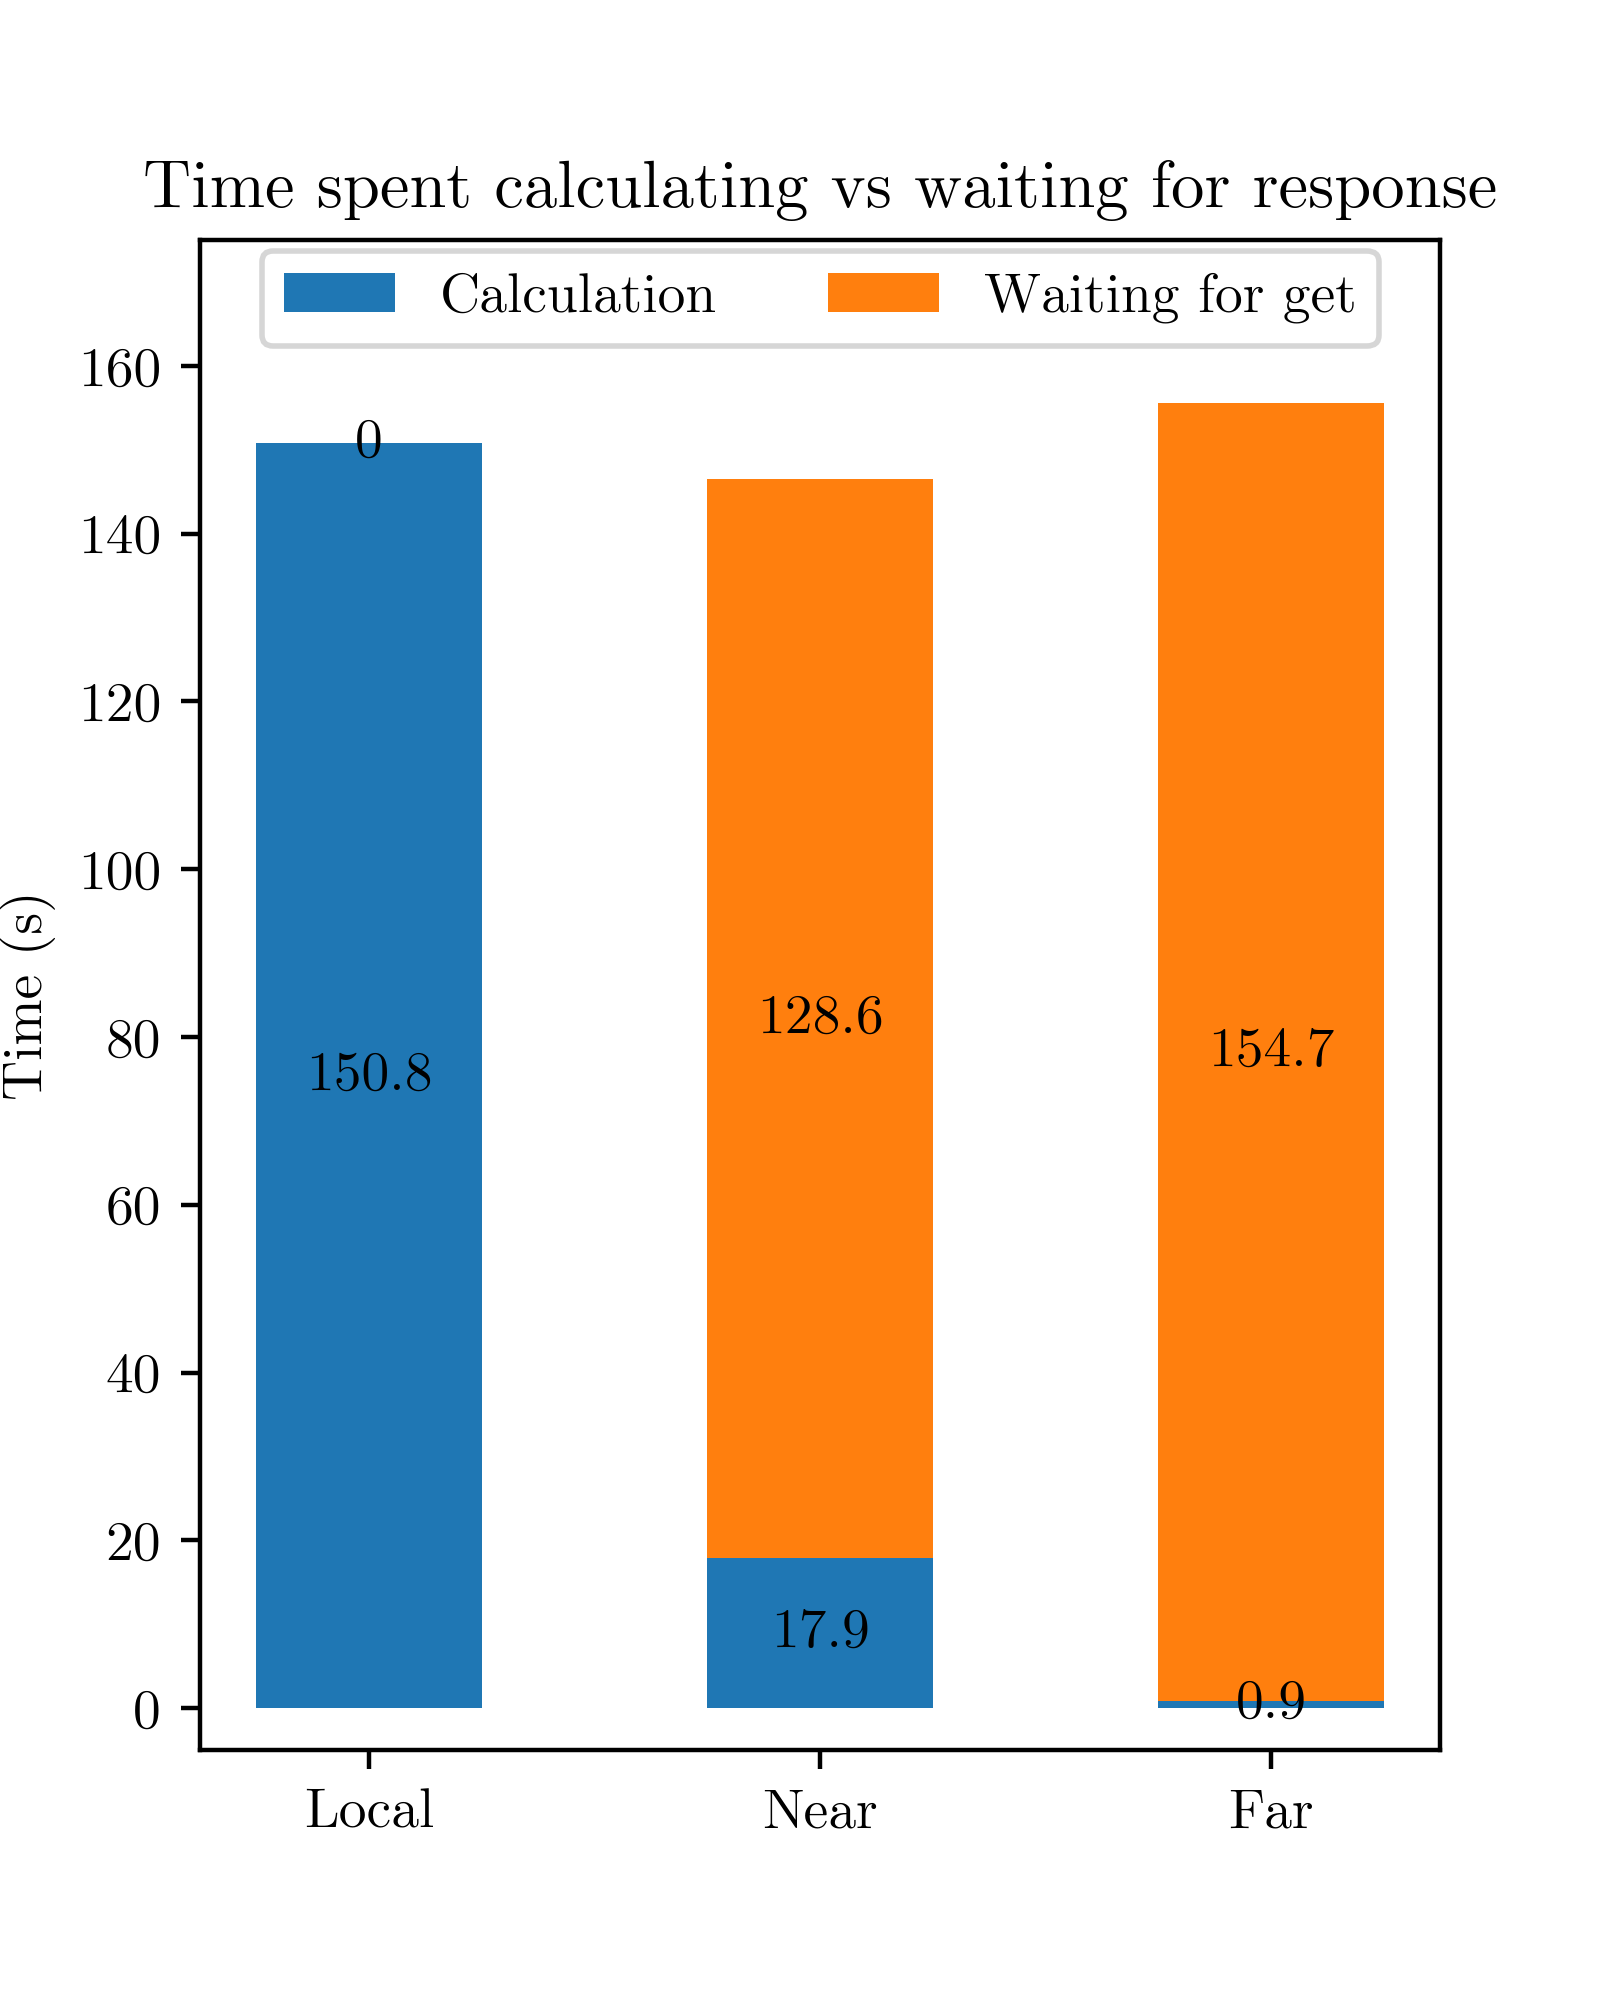
\includegraphics[scale=1]{chapters/evaluation/figures/bar_local_near_far_compare.png}
    \caption{Illustration of how much time is spent on waiting for data due to latency when using MEC Server.}
    \label{fig:bar_local_near_far}
\end{figure}

Figure \ref{fig:bar_local_near_far} shows how latency affect the the total time used when we have to constantly get data from the local device. It uses the same configuration as shown in table \ref{tab:MEC_partial_offloading_latency_balance}.


\begin{table}[h!]
    \centering
    \begin{tabular}[c]{|c|c|c|c|c|}
        \hline
        Node type & Limitation & Iterations & RTT to Local (ms)& Time used (s)\\
        \hline
        \hline
        Local & 30 & 850 & 0 & 28.0  \\
        \hline
        Near & 100 & 850 & 30 & 27.6 \\
        \hline
        Far & 300 & 8300 & 170 & 27.5 \\
        \hline
    \end{tabular}
    \caption{Partial offloading with a lot of communication between Local and Near, and little communication with Far.}
    \label{tab:MEC_partial_offloading_little}
\end{table}

Table \ref{tab:MEC_partial_offloading_little} shows the result of having high frequency of interaction between Local and Near, while having low frequency of interaction with Far.



\subsection{Discussion of results} \label{subsection:MEC_comparison}%Discussion of mec?
By comparing table \ref{tab:MEC_full_offloading_latency_balance} and \ref{tab:MEC_partial_offloading_latency_balance} we can see that we get faster results by using Partial offloading. Because the nodes work in parallel, the node who used the longest time shows how much time were used from start to end. Therefore, Partial offloading is the best solution for having fastest result when there is a lot of interaction.


Full offloading might for some devices be a requirement. The two most likely causes for this is if the Local device have very limited computational power, or need to save battery. Computation offloading is a great strategy to save energy, as sending data is usually not as expensive as computation. However, if we compare table \ref{tab:MEC_full_offloading_latency_balance} and \ref{tab:MEC_partial_offloading_latency_balance}, we can clearly see that using the local device will give results faster.

Table \ref{tab:MEC_partial_offloading_little} shows that using a strong Far node is beneficial as long as the interaction between Local or Near and Far is low. Additionally, figure \ref{fig:bar_local_near_far} shows that if the Near and Far node constantly have to get data from Local, the time to complete the whole task will be much slower. If you don't need to get info that often, then the Far server will yield better results as it has more computational power. In other words, the more interaction the better it is to use Local or Near node more. When there is little interaction then it is best to use the Far node more.

%nevn offloading. Vis stolpediagramm hvor en chunk av tiden er offloading. Vis også med N*latency?
%Bar chart med som viser hvor stor andel av de forskjellige utregningene som består av calulation og latency






\subsection{Characteristics}
\subsubsection{Control}
As discussed in section \ref{section:MEC_architecture}, the network architecture of MEC is up to the programmers. They can use NFV and SDN to control how each mobile device will be able to use the architecture. They can in other words use SDN and NFV to tailor the network to the context. Since VMs can be uploaded to surrounding MEC Servers, ensuring good \textit{relocation transparency} should be trivial. Due to SDN and NFV they could quickly redirect packets to new MEC Server when needed. The level of \textit{migration transparency} is therefore also left to developers.

\subsubsection{Offloading}
Since they use the cellular network to offload work, this architecture is well suited for IoT devices that can afford the latency. The cellular network is ubiquitous in modern society, and therefore it is optimal for IoT devices that move a lot, e.g. self-driving cars. When offloading they have to upload something, e.g. a VM, to the MEC Server. Alternatively they can make the MEC Server download from elsewhere. Since MEC uses VMs on the servers when offloading, the level of \textit{access transparency} is very good. The VMs ensure that the APIs for all the nodes are the same. Since cellular networks cover such a large area, \textit{location transparency} is trivial as the device can move quite a lot of distance before any migration is needed. If a node were to fail, it is up to the developers to ensure that other resources are available to recover from the failure. In other words, the level of \textit{failure transparency} is up to the programmers.

\subsubsection{Deployment}
MEC is easily horizontally scalable, as more MEC Servers can easily be added to cell towers. The only limit is how much power there is available and how much space there is available. If only a few servers is needed, then the cost is not too high either. It is also easily scalable in the sense that you can add more VMs to the MEC Server to help with offloading if needed. Another benefit of using VMs is that \textit{concurrency transparency} is easy to ensure as long as the MEC Server does not run out of resources. This is because they are in sperate VMs and should not affect each other.



%offloading
%    compute 
%    storage
%distribution
%    scaling
%Control


%tabell? subsections? idk

%TODO
% Gjøre målinger med overføring av filer først. Finn data på bandwidth og pluss det på tiden.
% Gjøre målinger hvor det kreves mer samhandling mellom nodene. Vi må se latency!


%\cite{mach_mobile_2017} for hvor mye som skal offloades.!!!!
% test med 100% offload, 50% offload osv
%\begin{itemize}
 %   \item Easily scalable as we have the common interface. This makes it easy to add more vms to run more apps. So, its horizontally scalable?
%\end{itemize}





% -------------------------------------------------------------------------------------------





\section{Cloudlets}
For Cloudlets we will also test with Full and Partial offloading like in section \ref{section:MEC_evaluation}. The same metrics for limitations for each type of node is also used. In total we want to do 10000 iterations spread over all the nodes.

\subsection{Full execution}
\begin{table}[h!]
    \centering
    \begin{tabular}[c]{|c|c|c|c|c|}
        \hline
        Node type & Limitation & Iterations & RTT to Local (ms)& Time used (s)\\
        \hline
        \hline
        Local           & 30 & 0 & 0 & 0  \\
        \hline
        Cloudlet(Near)  & 100 & 2800 & 3 & 30.2 \\
        \hline
        Far             & 300 & 7200 & 170 & 1285.0 \\
        \hline
    \end{tabular}
    \caption{Full offloading with communication.}
    \label{tab:Cloudlet_full_offloading_latency}
\end{table}
Table \ref{tab:Cloudlet_full_offloading_latency} shows the result of Full offloading to a nearby Cloudlet. We have used the same configuration as in table \ref{tab:MEC_full_offloading_balanced} to show how latency affects the result. 

\begin{table}[h!]
    \centering
    \begin{tabular}[c]{|c|c|c|c|c|}
        \hline
        Node type & Limitation & Iterations & RTT to Local (ms)& Time used (s)\\
        \hline
        \hline
        Local           & 30 & 0 & 0 & 0  \\
        \hline
        Cloudlet(Near)  & 100 & 9500 & 3 & 98.8 \\
        \hline
        Far             & 300 & 500 & 170 & 94.6 \\
        \hline
    \end{tabular}
    \caption{Full offloading with communication with more balance.}
    \label{tab:Cloudlet_full_offloading_latency_balanced}
\end{table}
Table \ref{tab:Cloudlet_full_offloading_latency_balanced} shows the result of a more balanced configuration with Full offloading in the sense that they used about the same time.




\subsection{Partial offloading}
\begin{table}[h!]
    \centering
    \begin{tabular}[c]{|c|c|c|c|c|}
        \hline
        Node type & Limitation & Iterations & RTT to Local (ms)& Time used (s)\\
        \hline
        \hline
        Local           & 30 & 850 & 0 & 28.1  \\
        \hline
        Cloudlet(Near)  & 100 & 2700 & 3 & 27.8 \\
        \hline
        Far             & 300 & 6450 & 170 & 1188.4 \\
        \hline
    \end{tabular}
    \caption{Partial offloading with communication.}
    \label{tab:Cloudlet_partial_offloading_latency}
\end{table}
Table \ref{tab:Cloudlet_partial_offloading_latency} shows the result of Partial offloading to a nearby Cloudlet. We have used the same configuration as in table \ref{tab:MEC_partial_offloading_balanced} to show how latency affects the result. 





\begin{table}[h!]
    \centering
    \begin{tabular}[c]{|c|c|c|c|c|}
        \hline
        Node type & Limitation & Iterations & RTT to Local (ms)& Time used (s)\\
        \hline
        \hline
        Local           & 30 & 2400 & 0 & 79.2  \\
        \hline
        Cloudlet(Near)  & 100 & 7150 & 3 & 73.3 \\
        \hline
        Far             & 300 & 450 & 170 & 75.2 \\
        \hline
    \end{tabular}
    \caption{Partial offloading with communication with more balance.}
    \label{tab:Cloudlet_partial_offloading_latency_balanced}
\end{table}
Table \ref{tab:Cloudlet_partial_offloading_latency_balanced} shows the result of a more balanced configuration with Partial offloading in the sense that they used about the same time.







\subsection{Decreasing interaction}
\begin{figure}[t]
    \centering
    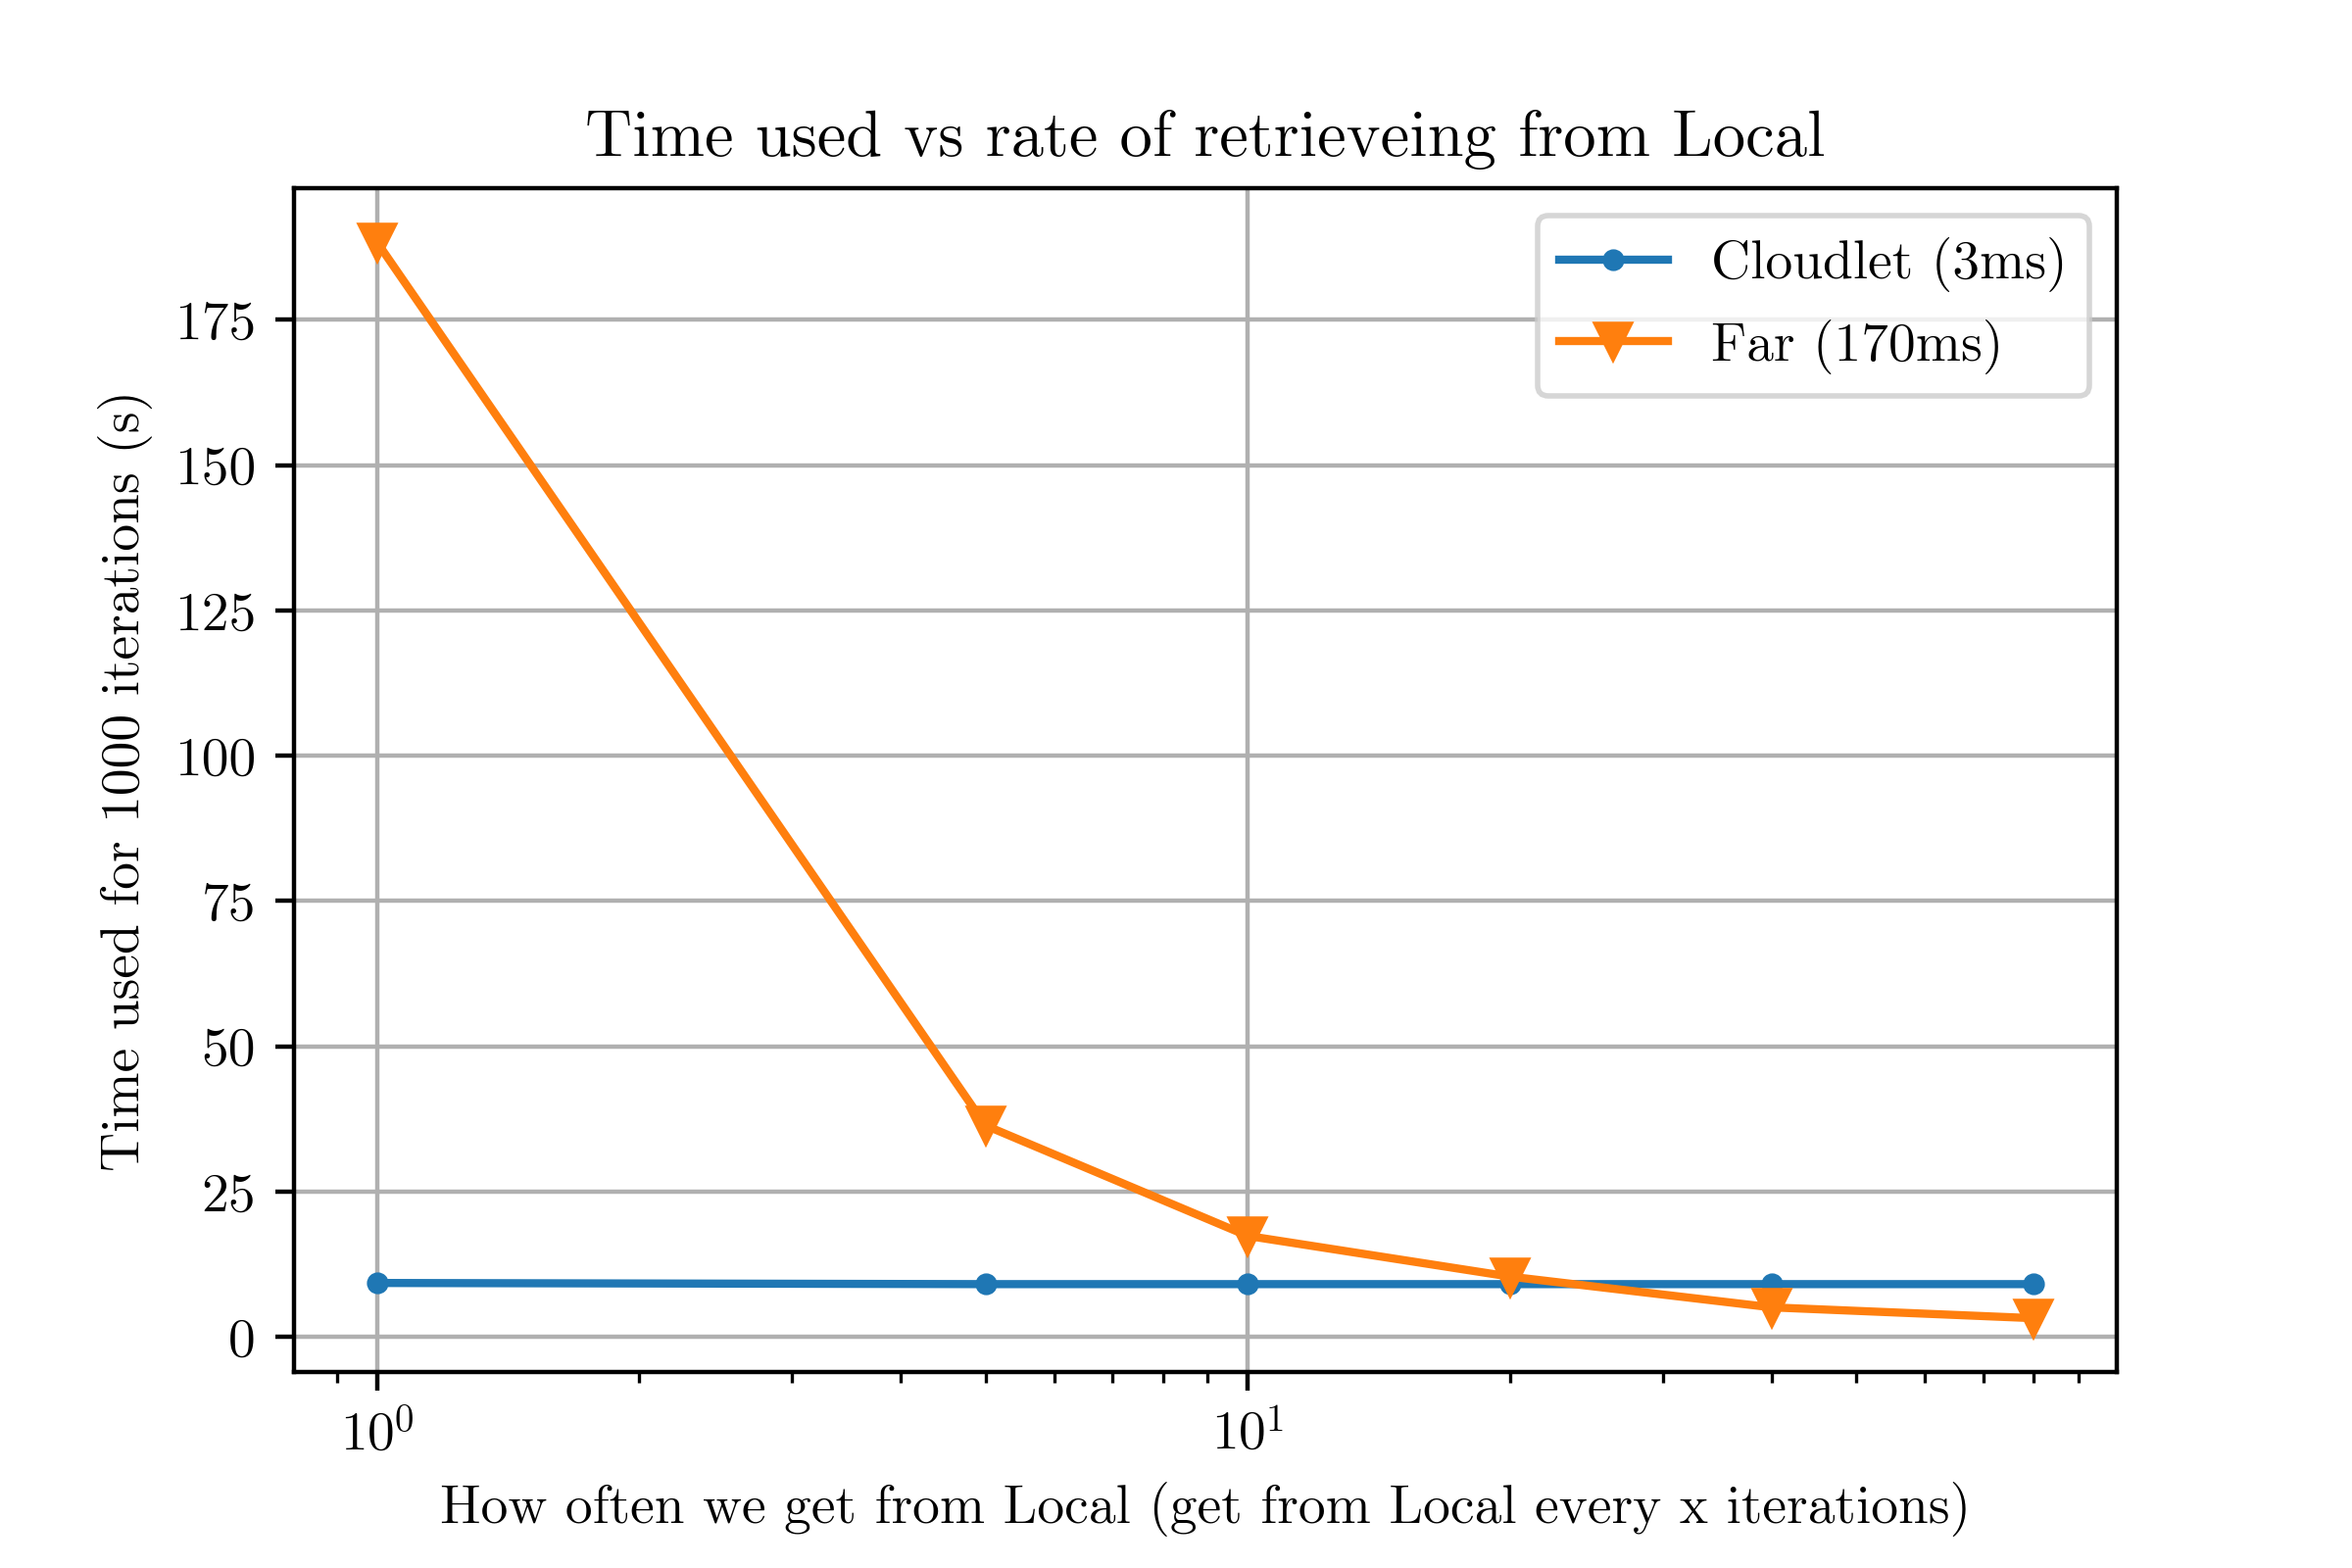
\includegraphics[scale=1]{chapters/evaluation/figures/Cloudlet_latency.png}
    \caption{Graph showing how interaction hurts. If x=10 then we get from Local every 10 iterations.}
    \label{fig:Cloudlet_latency_near_far_comparison}
\end{figure}
Figure \ref{fig:Cloudlet_latency_near_far_comparison} shows how the frequency of interaction between nodes will affect the time used, like shown for MEC in \ref{fig:time_graph_near_far}. 


\begin{figure}[t]
    \centering
    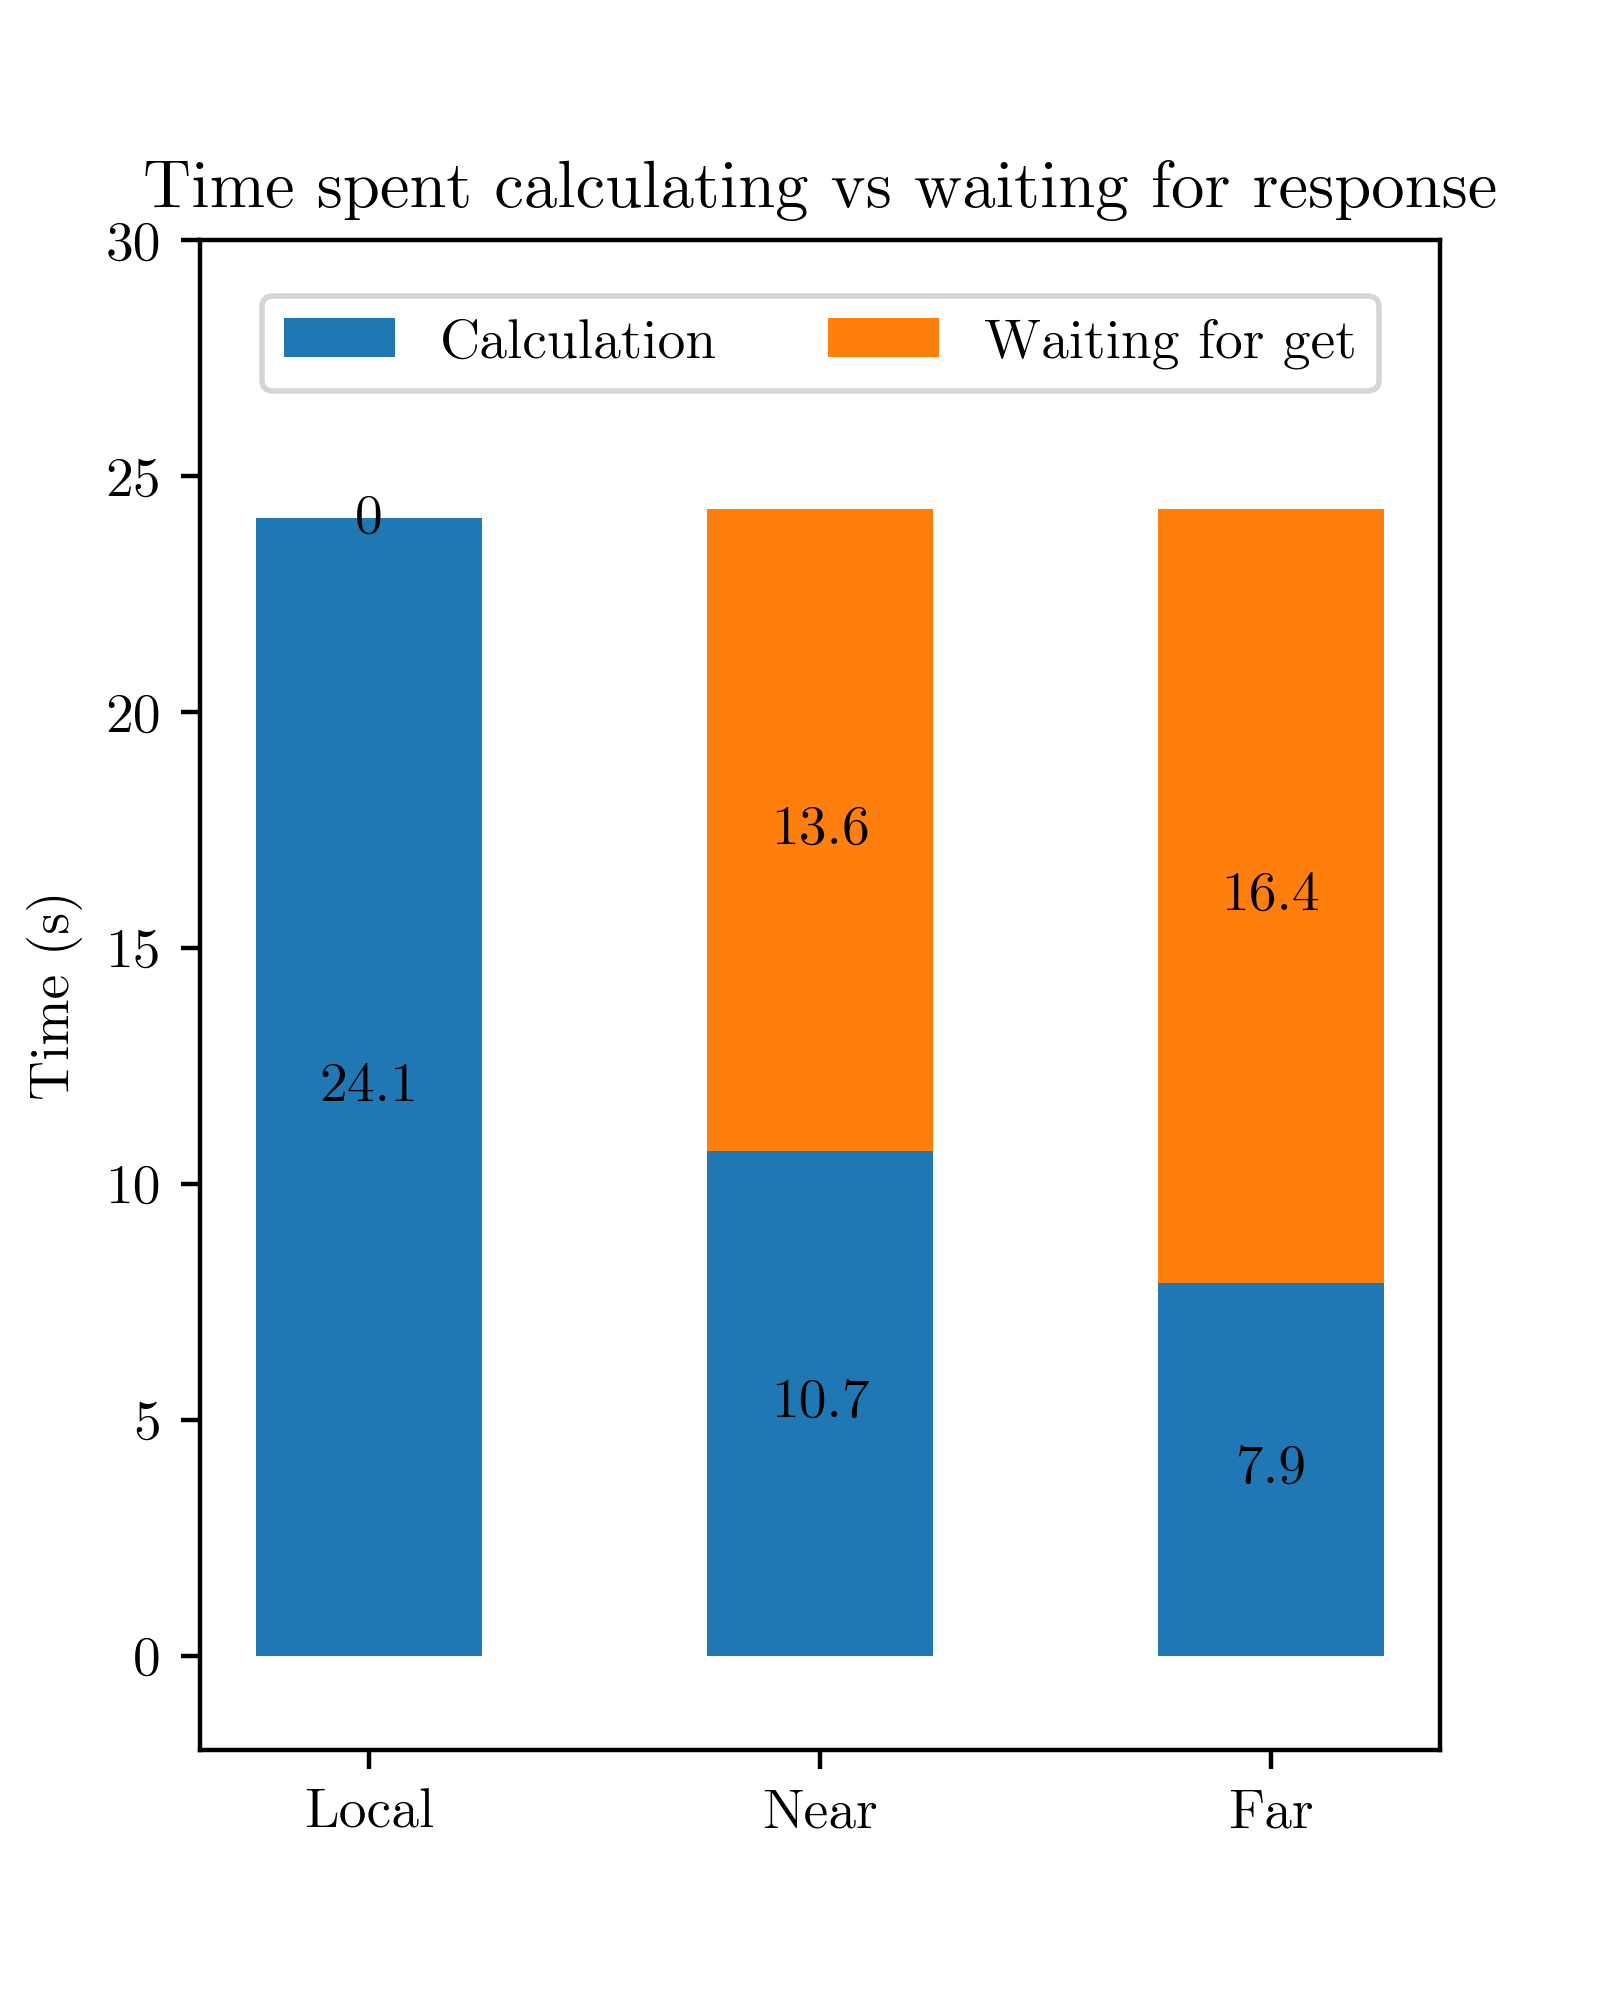
\includegraphics[scale=1]{chapters/evaluation/figures/bar_local_near_far_compare_low_interaction.png}
    \caption{Illustration of how much time is spent on waiting for data due to latency when using Cloudlets.}
    \label{fig:Cloudlet_latency_bar}
\end{figure}
Figure \ref{fig:Cloudlet_latency_bar} shows how much time used on waiting for data from Local, compared to how much time is used on calculating. The configuration used here is the same as shown in table \ref{tab:Cloudlet_partial_offloading_latency_balanced}.


\begin{table}[h!]
    \centering
    \begin{tabular}[c]{|c|c|c|c|c|}
        \hline
        Node type & Limitation & Iterations & RTT to Local (ms)& Time used (s)\\
        \hline
        \hline
        Local           & 30 & 750 & 0 & 24.1 \\
        \hline
        Cloudlet(Near)  & 100 & 2250 & 3 & 24.4 \\
        \hline
        Far             & 300 & 7000 & 170 & 24.3 \\
        \hline
    \end{tabular}
    \caption{Partial offloading with a lot of communication between Local and Near, and little communication with Far.}
    \label{tab:Cloudlet_partial_offloading_little_far}
\end{table}
Table \ref{tab:Cloudlet_partial_offloading_little_far} shows the result of offloading with high frequency to the Near node, while letting the Far node have bigger workloads, and therefore frequent interaction. 


\subsection{Discussion of results}
By comparing table \ref{tab:Cloudlet_full_offloading_latency_balanced} and \ref{tab:Cloudlet_partial_offloading_latency_balanced} we can see that we benefit from also using the Local device. However, if the device that is using the Cloudlets require Full offloading, then we still have significant speedup by offloading to the Cloudlet and the Far node compared to Local execution. Table \ref{tab:Cloudlet_partial_offloading_little_far} shows that using Far node as long as interaction is low, is also very beneficial.

Figure \ref{fig:Cloudlet_latency_near_far_comparison} shows that we can get better results by using Far in the situation where interaction between nodes is low. In other words, Cloudlets can benefit from using Far, but only when there is little communication needed. For fast response times we need to use the Cloudlet to do the computation. 

Figure \ref{fig:Cloudlet_latency_bar} shows that having minimal latency to a Near node is very beneficial. Even though almost half of the time is spent waiting, we have offloaded a significant amount of work. Table \ref{tab:Cloudlet_partial_offloading_little_far} 



\subsection{Characteristics}
\subsubsection{Control}
Controlling Cloudlets is done by the owner of each Cloudlet. Since Cloudlets are to be placed on locations, e.g. a coffee shop, then the owner of that location is able to configure the Cloudlet. The location owner can then limit usage and limit what kinds of applications are used on the Cloudlet. Handling failure and having good \textit{failure transparency} is mostly up to the programmer in Cloudlets. Should the Cloudlet fail, then a different near Cloudlet should take over, or in the worst case let the Local device handle it. 
\subsubsection{Offloading}
Cloudlets use \textit{dynamic VM synthesis} \cite{satyanarayanan_case_2009} to offload work. Essentially it means that we have to give the Cloudlet a VM to run the application. This makes \textit{access transparency} for Cloudlets quite good in theory. However, it gives an overhead which they reported to be quite high. This has likely been improved since 2009 as technology has improved. Bandwitdth, storage and computational power have significantly improved, which mitigates many of the issues they raised.
\subsubsection{Deployment}
Distribution is expensive for Cloudlets. Satyanarayanan et al\cite{satyanarayanan_case_2009} purposes different payment models, but each owner of a location has to decide if it is worth the investment. Since they are supposed to be ubiquitous, the total cost of having these readily available everywhere in society will be significant. If the Cloudlets are ubuiquitus, then the level of \textit{location and relocation transparency} is quite high. In their paper, they purpose a way of seamlessly migrating to other Cloudlets when needed. If this is accomplished, then the users of the local devices will not notice any drop in performance. Due to the ubiquitous nature of Cloudlets, having \textit{concurrency transparency} should not be a problem. Overloading all of the nearby Cloudlets will be a rare occurrence due to their ubiquitous nature.







% -------------------------------------------------------------------------------------------







\section{Google Anthos}
\subsection{Characteristics}
\subsubsection{Control}
Controlling the Anthos architecture is relatively easy as GCP will take care of all the difficult parts. You can control all the nodes in the Anthos control panel. This means that the one who owns the GCP account has full control over the nodes. The level of \textit{access  transparency} is quit high, as Anthos will take care of all the low-level problems. It is up to the programmer to decide how containers running on the platform will communicate. It also up to the programmer if they want users to be able to relocate objects. In other words \textit{migration transparency} is also up to the programmers.

\subsubsection{Offloading}
Since Anthos uses containers, offloading can be quite easy. However, it is up to the programmers to decide how offloading will work. Essentially, the Local device only needs to somehow contact the on-premises machines, for example through WiFi and LAN connections. The level of \textit{location transparency} is up to the programmers. It is dependent on how the containers are set up. Kubernetes is easily set up to manage \textit{replication and concurrency transparency}, as it lets you configure where the containers should reside, and how many of them should be there, as well as many other parameters.

\subsubsection{Deployment}
Deploying is relatively easy. As discussed earlier, you only need to install Anthos software on on-premises hardware and then configure Kubernetes to use it. Ensuring \textit{failure transparency} can be hard, but Kubernetes is configureable to handle failures. Essentially, it is up to the programmer to decide what happens if there is one.






% -------------------------------------------------------------------------------------------







\section{Amazon Cloudfront}
\subsection{Characteristics}
\subsubsection{Control}
Controlling Cloudfront is done in the Cloudfront control panel in the AWS console. Cloudfront lets you set up a wide array of features for your architecture. They provide DNS, NFV, Lambda@edge, Security, Sertificates, etc. All of this is controlled by the programmers in the AWS console.  


\subsubsection{Offloading}
AWS lets you set up servers, container software or Lambda@edge on Cloudfront. This lets gives a lot of freedom to the programmers on how they will set up the architecture. A downside of using AWS Lambda is that there is something called warm up time. It is pretty small, but can be notices in extreme latency-aware contexts. The warm up time depends on the programming language used, but it comes in addition to the latency towards the edge location. When it comes to \textit{concurrency, location and replication transparency}, it is up to the programmer, but are very easily adjustable. For example, for AWS Lambda, a single parameter can be change to let it scale more. AWS will handle scaling, the programmer just have to set the limit. When using server however, you have to add more servers to scale, so it is therefore more up to the programmers. The level of \textit{access transparency} is high, due to containerization and AWS Lambda. However, if servers are used, then the programmer have control of the access transparency level. \textit{Relocation and migration transparency} can be ensured by Cloudfront, unless you use the servers. Then it is up to the programmer to control it. 


\subsubsection{Deployment}
When setting up Cloudfront you do it trough the AWS control panel. You are restricted to use the edge servers that AWS provide. These servers are deployed all over the world. However, in some places there might be a long distance to the nearest server. Ensuring \textit{failure transparency} is handled by Cloudfront in this architecture. The programmer can focus more on what the program should do rather than focusing on what happens if it were to fail. 




% -------------------------------------------------------------------------------------------





\section{Akamai}
\subsection{Characteristics}
\subsubsection{Control}
Akamai features are controlled through Akamai's console. The level of \textit{access and migration transparency} is up to the programmer in this architecture.

\subsubsection{Offloading}
Akamai does offer ways of offloading, but they focus more on bringing content to the edge rather than just computation. Caching is the main purpose of Akamai edge servers, and using their edge servers for this ensures \textit{location, relocation, replication and concurrency transparency}. The level of \textit{replication transparency} is also somewhat up to the programmer, as the choose the locations of where they should cache the content.

\subsubsection{Deployment}
Setting up the edge servers are easily done through Akamai's console. You set up the edge server where you want it, and then push your content to that server. Akamai will take care of failures and will route requests to the original server if needed. This ensures \textit{failure transparency}. However, if the orginial server is very distant, then the client will most likely notice a drop in performance or response time.


% -------------------------------------------------------------------------------------------




\section{Discussion of findings}

\subsection{Comparing Cloudlets and MEC}
From the results we can see that if enough funding is available, then Cloudlets gives the best result. We can see that having low latency between Local and Near like the Cloudlet, is preferable for better results. However, one could argue that installation of MEC Servers are significantly easier and cheaper as you only install them at base stations that cover a wide area. When it comes to migration, it is significantly easier for MEC due to how much area is covered with cellular. If the mobile device were to move in the Cloudlet architecture then Cloudlets in the new location should already be ready to offload. This is hard, as with the frequency of Cloudlets it can be difficult to decide which Cloudlet to migrate to before it is too late. Since MEC cover such a large area, it should not be a problem to see when it is needed to migrate to other base stations. However, migration in MEC will likely take a longer time, as Cloudlets often will be on the same LAN and can therefore transfer faster and more reliably.

\subsection{Discussion of architectures}
Anthos is able to mimic the Cloudlet architecture by letting you set up on-premises servers. However, the Anthos nodes are confined to the owners environment, which is unlike the vision for Cloudlets. 

Cloudfront is a good choice as it is backed by a massive company, which has infrastructure in a lot of locations, and will likely expand in the future. It comes with the negative side effect of being confined to their locations, which in many cases might have too much latency.

Akamai is leading when it comes to content caching as they have the most infrastructure available. However, it is best used as a standard CDN, in the sense that you should offload web pages or other high volume data to their servers. Doing this will significantly improve the response time due to the lower latency, and will most likely give a smoother experience as there is less use of the Wide-area network.

A common thing for all architectures is that a lot of the control is up to the programmers. This allows for high customization of the application, as it is not limited to many constraints. Additionally, all the architectures allow for cooperation between Near nodes and Far nodes. 


\subsection{Offloading}
We can see from table \ref{tab:MEC_partial_offloading_little} and \ref{tab:Cloudlet_partial_offloading_little_far} that we do get a speed-up by using the Near-Far model, on the condition that the Far node does not do much latency-aware work. 

Every architecture that requires transferring of a VM or similar to the offloading node, will have an overhead. This overhead is mainly dependent on the size of the load that need to be transferred, the bandwidth between the Local and Near node, and the time it takes to start the VM or container. Context is required to know when to start offloading these VMs to the other nodes. If context is well known to the nodes, then they can start pre-loading to avoid having to wait for this overhead.







\section{The Near-Far Computing Model}
The Near-Far Computing Model is worth it in many cases. However, it is best utilized when you can have a Near node doing latency critical work, and having a Far node doing the latency non-critical work. For example, if the Local device is a smart device that need quick response on their data, it can offload to the Near node. When the Near node is done calculating, it can use the Far server to analyze the result as well as logging it. For storage, Near-Far is great for caching. Having caches that is closer to the client will result in way quicker results.

The common thing for all the discussed architectures is that they use a mix of both edge nodes and server nodes. They try as best as possible to use the edge nodes, but the distant strong data centers can aid when needed. 

If the Near node were to fail, then the Far node can take over. However, due to latency the Far node will give the client a worse experience if response time is critical. 

\subsection{Distribution Transparency}
In the following subsections we will discuss distribution transparency in Near-Far computing.

\subsubsection{Access Transparency}
When using the Near-Far model, one should use containerization or VMs to provide common API or middleware for all the nodes in the system. This ensures that developers does not have to deal with very low-level programming, and focus more on providing features and solutions.

\subsubsection{Location Transparency}
Location transparency is up to the programmer, but in most cases one should try to hide where objects are located. Due to the Near node having low latency, there should not be a problem to ensure that the location is hidden.

\subsubsection{Relocation Transparency}
Relocation transparency can be hard if the area where you are connected to the Near device is not big. For example, if you have to connect to a new node each time you enter a new room, ensuring relocation transparency can be hard. However, with good algorithms and enough knowledge about the context, it is possible. 

\subsubsection{Migration Transparency}
Migration transparency should not be difficult to implement. It is up to the programmer to decide how much level of transparency they want. 

\subsubsection{Replication Transparency}
Replication transparency is mostly up to the programmer. With enough Nodes available, the programmer can add or remove nodes as they see fit. It is up to the context if this will be noticed by the client. 

\subsubsection{Concurrency Transparency}
Concurrency transparency is also up to the programmer. In most cases however, it is best to avoid showing that multiple users are using the same resources. For example, one should not notice that several others are watching the same content as you are. 

\subsubsection{Failure Transparency}
If enough nodes are available, then recovering from a failure should have minimal impact on the user. However, if the application in question is latency-aware and is forced to use Far or Local resources to do these time critical operations, then the client will suffer. However, one should quickly be able to recover to the previous state.

\subsection{Definition}
The Near-Far Computing is a superset, or a spectrum that covers all models or architecutres that focuses on mitigating latency issues by using Near nodes and Far nodes. 



\section{Summary}
In this chapter we have tested MEC and Cloudlets with the program described in implementation. We have also discussed characteristics of all the architectures. We have discussed how these characteristics relate to the Near-Far Computing Model. Finally we have provided a definition for the Near-Far Computing Model



\section{TODO}

Sometimes the result of the far is not relevant for the near. We can also let the near compute while the far stores data.

Near-Far computing is applicable where there is not much need for interaction between the Far node and the Local or Near node.


%evaluation of architecture using the method described in "Design of experiments" chapter


\chapter{Results}                     %% ... or ??

\chapter{Conclusion}                     %% ... or Konklusjon
%% future work!!
\section{Future work}
%Developing a real example using Augmented Reality or some other latency-aware application would be a good way to show that our solution work in more than just a simulation. This can hopefully be done when a new Emerald compiler with no memory limitation is available.

\backmatter{}
\printbibliography
\end{document}
